Este capítulo descreve como a plataforma foi construída a partir da arquitetura apresentada no Capítulo~\ref{cap:modelagem}. A Seção~\ref{sec:interpretador-nucleo} situa o interpretador, desenvolvido em conjunto com o trabalho complementar. As Seções~\ref{sec:customizacao-dinamica} a~\ref{sec:sistema-correcao} tratam da customização da linguagem, da edição de código, da execução das análises a partir da IDE, do terminal e do sistema de correção automatizada. A Seção~\ref{sec:acessibilidade-responsividade} reúne acessibilidade, responsividade e internacionalização, a Seção~\ref{sec:orientacao-usuario} descreve os recursos de orientação ao usuário e a Seção~\ref{sec:telas-plataforma} apresenta as telas da plataforma na ordem dos requisitos funcionais. Os testes estão no Capítulo~\ref{cap:testes}.

\section{Interpretador}
\label{sec:interpretador-nucleo}

O interpretador constitui o núcleo de tradução comum a este projeto e foi desenvolvido de forma colaborativa pelos dois autores, Victor de Souza Vilela da Silva e Igor Lamoia Queiroz, conforme a divisão de responsabilidades registrada no Apêndice~\ref{ap:plano}. Implementado em TypeScript e consumido pela IDE como dependência local, conforme descrito na Seção~\ref{sec:arquitetura-plataforma}, o núcleo encadeia as fases de análise léxica, análise sintática, geração de código intermediário em três endereços e execução pelo interpretador, recebendo dinamicamente a configuração da linguagem definida pelo usuário (palavras-chave, operadores em forma de palavra, literais booleanos, delimitadores de bloco e terminador de instrução).

Por se tratar da base técnica compartilhada entre os dois textos, o detalhamento interno de cada fase do núcleo, incluindo as estratégias de varredura léxica, a análise sintática por descida recursiva, a geração de código de três endereços e o funcionamento do interpretador, é objeto do trabalho complementar de autoria de Victor de Souza Vilela da Silva. Este texto concentra-se na forma como a IDE aciona e integra esse núcleo, detalhada nas seções seguintes.

\section{Customização Dinâmica de \textit{Tokens} e Sintaxe}
\label{sec:customizacao-dinamica}

A funcionalidade central da plataforma, que consiste na possibilidade de o usuário personalizar dinamicamente a sintaxe e o vocabulário da linguagem, foi materializada em um conjunto coordenado de componentes, \textit{contexts} e utilitários. O elemento central dessa funcionalidade é o \texttt{KeywordContext}, um \textit{context} do React que mantém, em memória e na camada de armazenamento local do navegador, o estado completo da customização ativa, incluindo o mapeamento de palavras-chave personalizadas, os operadores em forma de palavra, os literais booleanos, os delimitadores de bloco e o terminador de instrução.

O contrato técnico que sustenta a customização é definido pelo módulo \texttt{config.ts} do pacote \texttt{compiler}, que declara, por meio de tipos TypeScript, todos os elementos da linguagem passíveis de personalização. O Trecho de Código~\ref{lst:lexer-config} apresenta esses tipos, que funcionam como a interface formal entre a camada de interface, responsável pela coleta das preferências do usuário, e o núcleo do tradutor, responsável pela aplicação da configuração no momento da varredura léxica.

\begin{lstlisting}[language=typescript, caption={Tipos que descrevem a configuração customizável do lexer.}, label={lst:lexer-config}, captionpos=b]
export type KeywordMap = Record<string, number>;

export type OperatorWordMap = {
  logical_or?: string;     logical_and?: string;
  logical_not?: string;    less?: string;
  less_equal?: string;     greater?: string;
  greater_equal?: string;  equal_equal?: string;
  not_equal?: string;
};

export type BooleanLiteralMap = {
  true?: string;
  false?: string;
};

export type LexerBlockDelimiters = {
  open: string;
  close: string;
};

export type LexerConfig = {
  customKeywords?: KeywordMap;
  operatorWordMap?: OperatorWordMap;
  booleanLiteralMap?: BooleanLiteralMap;
  statementTerminatorLexeme?: string;
  blockDelimiters?: LexerBlockDelimiters;
  locale?: string;
  indentationBlock?: boolean;
  tabWidth?: number;
};
\end{lstlisting}

A definição de quais elementos da linguagem seriam exibidos como configuráveis foi guiada pelos achados empíricos de \citeonline{stefik2013}, segundo os quais a sintaxe tradicional derivada da família C atua como uma barreira significativa para estudantes iniciantes. Foram disponibilizadas para customização as palavras-chave de declarações de tipo (\texttt{int}, \texttt{float}, \texttt{bool}, \texttt{string}), de controle de fluxo (\texttt{if}, \texttt{else}, \texttt{for}, \texttt{while}, \texttt{break}, \texttt{continue}, \texttt{return}, \texttt{switch}, \texttt{case}), as operações de entrada e saída (\texttt{print}, \texttt{scan}), os operadores lógicos (\texttt{\&\&}, \texttt{||}, \texttt{!}) e relacionais (\texttt{==}, \texttt{!=}, \texttt{>}, \texttt{>=}, \texttt{<}, \texttt{<=}), os literais booleanos (\texttt{true}, \texttt{false}), os delimitadores de bloco (chaves ou indentação) e o terminador de instrução. Essas opções abrangem precisamente os elementos que oneram a carga cognitiva inicial discutidos por \citeonline{stefik2013}, mantendo intactos os aspectos estruturais responsáveis pela consistência das demais fases do compilador.

A consolidação do estado da customização no \texttt{KeywordContext} é exposta às demais camadas da aplicação por meio do utilitário \texttt{buildLexerConfig}, apresentado no Trecho de Código~\ref{lst:build-lexer-config}. Esse utilitário traduz o estado em memória, contendo os mapeamentos de palavras-chave, os operadores, os literais booleanos, os delimitadores de bloco e o terminador de instrução, em um descritor compatível com o tipo \texttt{LexerConfig} do pacote \texttt{compiler}, atuando como a fronteira efetiva entre o estado da interface e a invocação do tradutor.

\begin{lstlisting}[language=typescript, caption={Utilitário \texttt{buildLexerConfig} do \texttt{KeywordContext}, que materializa a configuração corrente em um descritor consumível pelo lexer.}, label={lst:build-lexer-config}, captionpos=b]
const buildKeywordMap = useCallback((): Record<string, number> => {
  const map: Record<string, number> = {};
  for (const m of customization.mappings) {
    map[m.custom] = m.tokenId;
  }
  return map;
}, [customization.mappings]);

const buildLexerConfig = useCallback((): IDECompilerConfigPayload => {
  return buildLexerConfigFromCustomization(customization);
}, [customization]);
\end{lstlisting}

A interface de customização foi implementada como um assistente progressivo no formato \textit{wizard}, materializado no componente \texttt{keyword-customizer}, que conduz o usuário por etapas independentes, cada uma responsável por um aspecto específico da personalização. O fluxo é controlado pelo \texttt{wizard-model}, que mantém o estado de navegação e valida cada passo antes de permitir o avanço. A declaração formal das etapas do assistente é apresentada no Trecho de Código~\ref{lst:wizard-steps}, no qual cada elemento do arranjo \texttt{WIZARD\_STEPS} associa um identificador, um título exibido na barra de progresso, uma descrição textual e um ícone semântico, oferecendo ao usuário um mapa visual contínuo do fluxo de personalização.

\begin{lstlisting}[language=typescript, caption={Declaração do arranjo \texttt{WIZARD\_STEPS}, que organiza as etapas do assistente de personalização.}, label={lst:wizard-steps}, captionpos=b]
export const WIZARD_STEPS = [
  { id: "identity",  title: "Identidade",
    description: "Escolha o ponto de partida da linguagem.",
    icon: "fingerprint" },
  { id: "IO",        title: "Entrada/Saida",
    description: "Defina saida, leitura e a linguagem das variaveis.",
    icon: "cable" },
  { id: "types",     title: "Tipagem",
    description: "Defina leitura, escrita e o vocabulario usado para declarar variaveis.",
    icon: "book-open-text" },
  { id: "structure", title: "Estrutura",
    description: "Configure blocos, delimitadores e o fim das instrucoes.",
    icon: "blocks" },
  { id: "rules",     title: "Operadores",
    description: "Ajuste os operadores, literais booleanos e regras de decisao.",
    icon: "sigma" },
  { id: "flow",      title: "Fluxo",
    description: "Customize o vocabulario de controle.",
    icon: "route" },
  { id: "review",    title: "Revisao",
    description: "Confira o resumo final antes de salvar.",
    icon: "clipboard-check" },
] as const;
\end{lstlisting}

A cada alteração proposta pelo usuário, o componente \texttt{preview-builder} produz, em tempo real, um trecho de código exemplificativo que reflete a customização corrente, oferecendo uma visualização imediata do impacto das mudanças sobre a aparência dos programas. O Trecho de Código~\ref{lst:preview-builder} ilustra a função \texttt{buildDelimiterSnippet}, responsável por interpolar, em um molde fixo, as palavras-chave e os delimitadores efetivamente escolhidos pelo usuário, produzindo um trecho ilustrativo com a configuração corrente.

\begin{lstlisting}[language=typescript, caption={Função \texttt{buildDelimiterSnippet}, que gera o \textit{preview} dinâmico exibido durante a personalização.}, label={lst:preview-builder}, captionpos=b]
export function buildDelimiterSnippet(
  draft: StoredKeywordCustomization,
): string {
  const print = getKeyword(draft, "print");
  const scan = getKeyword(draft, "scan");
  const lineEnding = buildLineEnding(draft);
  const functionKeyword = getKeyword(draft, "function");
  const baseCodeSnippet = `${functionKeyword} main()`;

  const open = draft.blockDelimiters.open.trim() || "{";
  const close = draft.blockDelimiters.close.trim() || "}";

  return `${baseCodeSnippet}${open}\n\t${print}("Ola Mundo!")${lineEnding}
  ${scan}(nome)${lineEnding}\n\t${print}("Me chamo:", nome)\n${close}`;
}
\end{lstlisting}

A pré-visualização permite inspecionar a escrita resultante antes de salvar a configuração. A avaliação desse recurso pelo painel de especialistas é apresentada na Seção~\ref{sec:resultado-assistente}.

A validação das customizações é centralizada em um conjunto de funções utilitárias dedicadas, hospedadas no diretório \texttt{contexts/keyword/keyword-validator.ts}. A função \texttt{validateCustomKeyword} garante que palavras-chave personalizadas atendam às restrições léxicas elementares e não colidam entre si; \texttt{validateBlockDelimiters} verifica a consistência dos delimitadores de bloco. Toda a verificação ocorre de forma preventiva, no momento da alteração pelo usuário, impedindo que configurações inválidas sejam persistidas ou propagadas ao analisador léxico, em conformidade com os princípios de detecção precoce de erros discutidos por \citeonline{cooper2012}.

O Trecho de Código~\ref{lst:validate-delimiters} ilustra a estratégia de verificação aplicada aos delimitadores de bloco. A função encadeia as restrições elementares (ambos os delimitadores preenchidos, ausência de espaços, distinção entre o delimitador de abertura e o de fechamento e ausência de colisão com palavras reservadas), devolvendo, em caso de violação, a mensagem internacionalizada correspondente. Até setembro, a segunda verificação exigia forma de identificador, com \texttt{WORD\_REGEX}. Ela foi trocada por \texttt{DELIMITER\_REGEX}, que recusa apenas espaços, para que a predefinição livre do assistente pudesse informar as próprias chaves como delimitadores. Com isso a interface aceita também delimitadores como \texttt{<:} e \texttt{:>}, que o analisador léxico do núcleo não reconhece como um único \textit{token}; a limitação está descrita no texto complementar. Quando todas as restrições são atendidas, a função retorna \texttt{null}, sinalizando à interface que a configuração pode ser persistida.

\begin{lstlisting}[language=typescript, caption={Função \texttt{validateBlockDelimiters}, responsável pela verificação preventiva dos delimitadores de bloco.}, label={lst:validate-delimiters}, captionpos=b]
export function validateBlockDelimiters(
  value: BlockDelimiters,
): string | null {
  const open = value.open.trim();
  const close = value.close.trim();

  if (!open && !close) return null;
  if (!open || !close) {
    return ui.validation_fill_delimiters;
  }

  if (!DELIMITER_REGEX.test(open) || !DELIMITER_REGEX.test(close)) {
    return ui.validation_invalid_delimiter_format;
  }

  if (open === close) {
    return ui.validation_delimiters_must_differ;
  }

  if (
    ORIGINAL_KEYWORDS.includes(open) ||
    ORIGINAL_KEYWORDS.includes(close)
  ) {
    return ui.validation_delimiters_reserved;
  }

  return null;
}
\end{lstlisting}

\subsection{Linguagens predefinidas e identidade da configuração}

A IDE oferece quatro linguagens prontas no seletor, definidas em \texttt{lib/default-languages.ts}: Portugol, Python-like, C-like e Ruby-like. Portugol é a configuração inicial quando não há uma configuração salva aplicável. Essas opções combinam vocabulário e modos já implementados no núcleo; seus nomes indicam inspiração sintática, sem equivalência com as linguagens de propósito geral. A Tabela~\ref{tab:linguagens-predefinidas} resume os modos escolhidos por cada opção.

\begin{table}[htbp]
\centering
\caption{Configurações predefinidas disponíveis no seletor da IDE.}
\label{tab:linguagens-predefinidas}
\footnotesize
\renewcommand{\arraystretch}{1.15}
\begin{tabular}{|p{2.3cm}|p{2.8cm}|p{4cm}|p{4cm}|}
\hline
\textbf{Configuração} & \textbf{Blocos} & \textbf{Tipagem e arranjos} & \textbf{Terminador} \\\hline
Portugol & \texttt{inicio}/\texttt{fim} & Tipos explícitos; arranjos fixos & Ponto e vírgula obrigatório \\\hline
Python-like & Indentação & Sem declaração explícita de tipo; arranjos dinâmicos & Opcional no fim da linha \\\hline
C-like & Chaves & Tipos explícitos; arranjos fixos & Ponto e vírgula obrigatório \\\hline
Ruby-like & \texttt{do}/\texttt{end} & Sem declaração explícita de tipo; arranjos dinâmicos & Opcional no fim da linha \\\hline
\end{tabular}
\legend{Fonte: elaborado pelo autor a partir de \texttt{default-languages.ts}.}
\end{table}

O \textit{hook} \texttt{useLanguageChoices} reúne essas quatro opções com as linguagens locais do visitante ou com o acervo remoto do usuário autenticado. Selecionar uma opção predefinida aplica sua configuração e grava a escolha no armazenamento local, sem criar uma linguagem no banco. Para uma linguagem remota, o \textit{hook} recupera o detalhe e solicita a atualização da linguagem ativa pela API. As predefinições do seletor são distintas dos pontos de partida do assistente, definidos em \texttt{wizard-model.ts}, que incluem também as opções livre e inspirada no vocabulário mineiro.

Nas declarações sem tipo explícito, as palavras canônicas são \texttt{variable}, que declara uma variável, e \texttt{function}, que declara uma função. Versões anteriores da configuração usavam como palavras canônicas \texttt{variavel} e \texttt{funcao}, que designam os mesmos dois elementos. Neste texto, portanto, \texttt{variavel} equivale a \texttt{variable}, e \texttt{funcao} equivale a \texttt{function}. Os termos em português continuam disponíveis como personalizações, e a predefinição Portugol os utiliza; a normalização de configurações armazenadas reconhece as chaves antigas e as converte para as atuais, preservando os lexemas escolhidos. O reconhecimento de identificadores e a validação dos nomes personalizados passaram a admitir também \texttt{ç} e \texttt{Ç}, além das letras latinas sem acento e do sublinhado; dígitos são aceitos após o primeiro caractere. Isso não corresponde a aceitar qualquer caractere Unicode.

O assistente mantém nome e descrição nos campos \texttt{name} e \texttt{description}. A edição de uma linguagem existente usa a rota \texttt{/language-creator/[id]}, cujo carregamento inicial ocorre no servidor por \texttt{getServerSideProps}: o identificador é validado, a credencial do \textit{cookie} é encaminhada à API e os dados retornados inicializam o formulário. A criação sem identificador continua disponível sem autenticação, com persistência local. Essa distinção evita tratar a edição remota como uma simples reabertura de um rascunho local.

A persistência da customização foi modelada em duas camadas complementares. As configurações ativas no editor são salvas localmente, no \textit{localStorage} do navegador, por meio do utilitário \texttt{keyword-language-storage}, garantindo que o estado da personalização sobreviva ao recarregamento da página e à navegação entre rotas da aplicação. Linguagens nomeadas e exportadas pelo usuário, por sua vez, são persistidas no \textit{back-end} via API, viabilizando o compartilhamento entre dispositivos e a vinculação de linguagens específicas a exercícios oferecidos pelo professor. O utilitário \texttt{language-creator-navigation} orquestra as transições entre as etapas de criação, gravação e ativação de linguagens, mantendo coesão entre o estado em memória, o estado no \textit{localStorage} e o estado remoto.

Por fim, o impacto visual imediato da customização sobre o editor Monaco é mediado pela função \texttt{updateJavaMMKeywords}. Essa função reconstrói dinamicamente a gramática léxica registrada no editor cada vez que o \texttt{KeywordContext} sinaliza uma alteração na customização, refletindo de imediato o realce de sintaxe, a sugestão automática de palavras-chave e a documentação contextual exibida pelo Monaco. O Trecho de Código~\ref{lst:update-monaco} apresenta sua assinatura, evidenciando o desacoplamento entre o módulo de personalização e o módulo de edição: a função recebe a instância do Monaco, o conjunto atualizado de mapeamentos e as opções de linguagem, delegando à função interna \texttt{registerJavaMMLanguage} o registro completo do dialeto sob o identificador \texttt{java--}. Essa abordagem evita a necessidade de reinicializar o editor a cada mudança e preserva a instância do editor durante a personalização.

\begin{lstlisting}[language=typescript, caption={Função \texttt{updateJavaMMKeywords}, ponto de integração entre o estado da customização e o Monaco Editor.}, label={lst:update-monaco}, captionpos=b]
export const JAVAMM_LANGUAGE_ID = "java--";

export type JavaMMKeywordMapping = {
  original: string;
  custom: string;
  tokenId: number;
};

export function updateJavaMMKeywords(
  monaco: typeof monacoEditor,
  keywordMappings: JavaMMKeywordMapping[],
  options: JavaMMLanguageOptions = {},
) {
  registerJavaMMLanguage(monaco, keywordMappings, options);
}
\end{lstlisting}

\section{Edição de Código e Sistema de Arquivos Virtual}
\label{sec:edicao-codigo}

A experiência de edição foi construída em torno do \textit{Microsoft Monaco Editor}, o mesmo motor de edição utilizado pelo Visual Studio Code, integrado à aplicação por meio do pacote \texttt{@monaco-editor/loader}. A linguagem personalizada do projeto foi registrada sob o identificador \texttt{java--}, e dois temas próprios, \texttt{editor-glass-dark} e \texttt{editor-glass-light}, foram modelados a partir do módulo \texttt{EditorThemes.ts} para harmonizar visualmente o editor com o restante da identidade da plataforma, em ambas as variações de tema claro e escuro.

O gerenciamento do editor foi encapsulado no \texttt{EditorContext}, que abriga a referência da instância Monaco, o código-fonte corrente, o nome do arquivo ativo, os marcadores de linha utilizados para destacar erros e o conjunto de configurações de exibição. A interação entre o usuário e o editor foi enriquecida pelo \textit{hook} \texttt{useDebugger}, responsável por sinalizar visualmente, durante a execução passo a passo, qual instrução do código intermediário está sendo processada pelo interpretador, em consonância com o requisito pedagógico de tornar visível o processo de tradução.

A persistência local dos arquivos do usuário foi modelada pelo \textit{hook} \texttt{useFileSystem}, que implementa um sistema de arquivos virtual sustentado pelo \textit{localStorage} do navegador. Essa abordagem permite que múltiplos arquivos sejam criados, renomeados, removidos e alternados sem qualquer dependência de servidor remoto, permitindo trabalhar com documentos locais após o carregamento da aplicação, sem comprovar funcionamento integral \textit{offline}. O \textit{hook} \texttt{useEditorWithFileSystem} combina o estado do editor com o sistema de arquivos virtual, garantindo a sincronização bidirecional entre o conteúdo exibido no Monaco e o conteúdo persistido localmente. Complementarmente, os \textit{hooks} \texttt{useExplorer} e \texttt{useSearch} oferecem, no painel lateral, navegação por estrutura de arquivos e busca textual sobre todos os arquivos do projeto, replicando as funcionalidades essenciais de uma IDE profissional.

O painel lateral da IDE, implementado em \texttt{SidebarPanel}, reúne as visões de arquivos, busca, linguagem e depuração em uma composição cuja largura pode ser ajustada por arraste. O componente mantém a largura durante sua montagem e aplica um limite mínimo conforme a largura da janela. O ajuste usa eventos de ponteiro. A revisão também adotou cores derivadas do tema em formulários, painéis e tabelas, cujos resultados de contraste no recorte testado são apresentados na Seção~\ref{subsec:verificacao-interface}.

A Figura~\ref{fig:ide-execucao} mostra a IDE na área de resolução de exercícios, com a linguagem Didática em Português ativa. No painel da IDE, à esquerda fica o explorador do sistema de arquivos virtual; ao centro, o editor com o arquivo \texttt{main.?}, em que \texttt{numero\_inteiro}, \texttt{leia}, \texttt{se} e \texttt{inicio} recebem o destaque de palavra reservada; abaixo, o terminal com uma execução do programa. As capturas desta seção e das seguintes foram feitas em 20 de outubro de 2026, na execução local da plataforma, com as contas de demonstração do \textit{seed} e uma lista criada para o registro, travada na linguagem predefinida Didática em Português.

\begin{figure}[htbp]
    \centering
    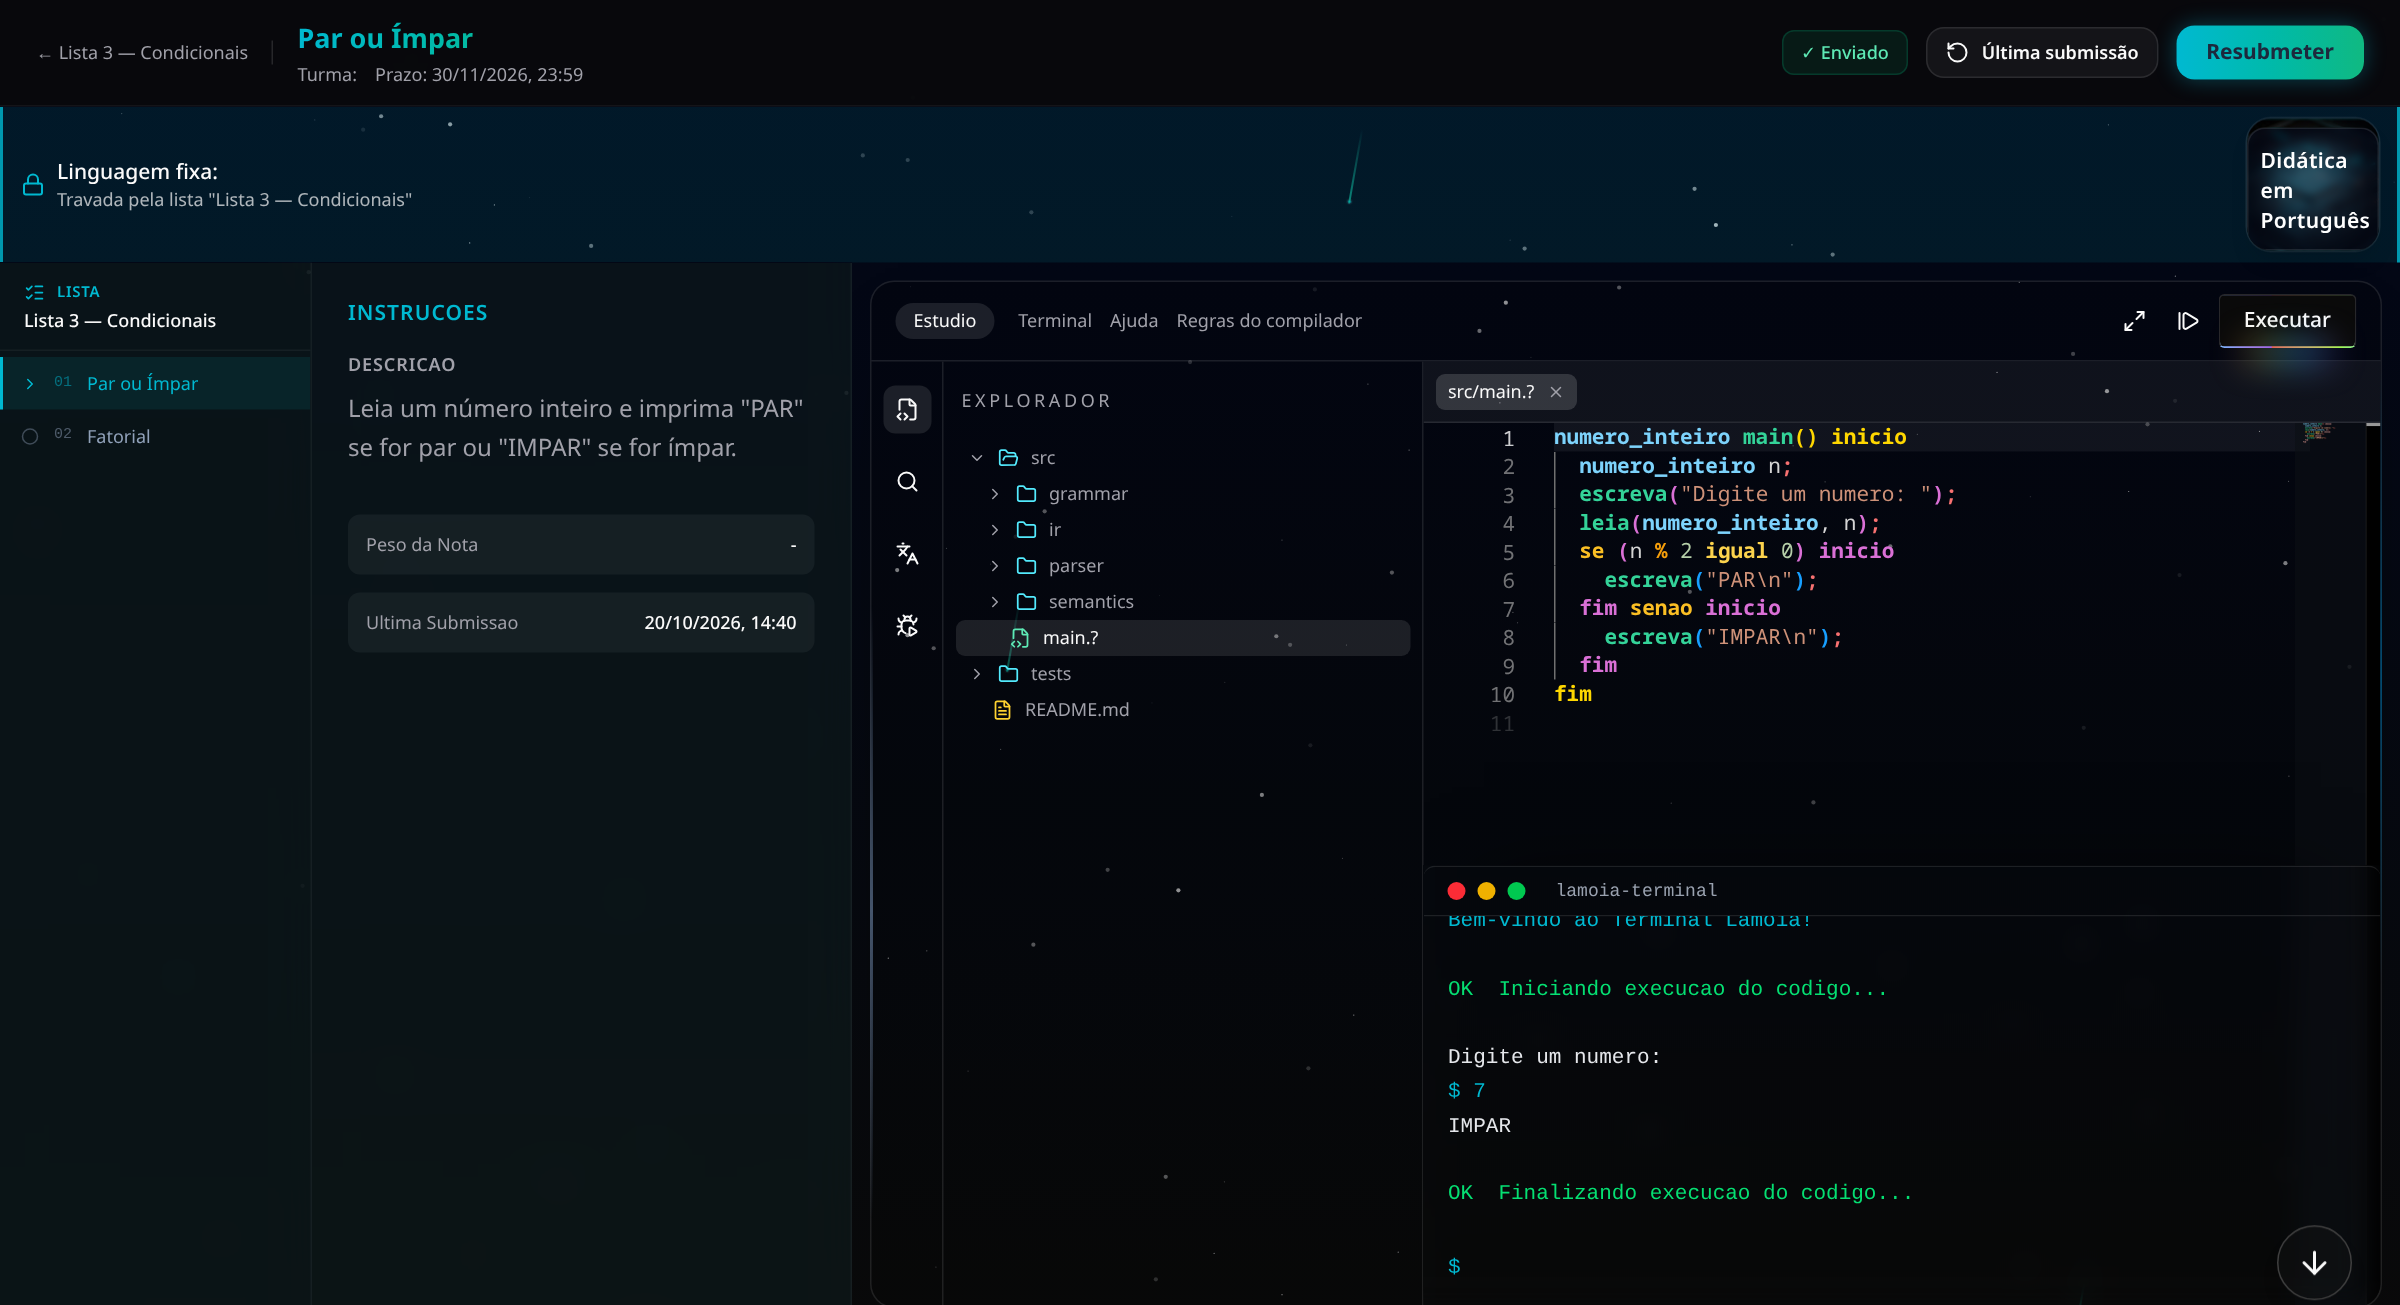
\includegraphics[width=\textwidth,height=0.42\textheight,keepaspectratio]{IDE/execucao_terminal.png}
    \caption{IDE com a linguagem Didática em Português ativa e o terminal após uma execução.}
    \label{fig:ide-execucao}
    \legend{Fonte: elaborado pelo autor.}
\end{figure}

\section{Execução das Análises Léxica e Sintática a partir da IDE}
\label{sec:execucao-analises}

A invocação das análises do compilador a partir da IDE foi modelada por meio de \textit{hooks} dedicados que encapsulam toda a interação entre a camada de interface e o núcleo de tradução. Diferentemente da estratégia adotada por ferramentas como a plataforma Laila, discutida no Capítulo~\ref{cap:trabalhos-relacionados}, na qual o código submetido pelo usuário é encaminhado a um serviço remoto para processamento, neste trabalho a execução das análises foi modelada inteiramente no navegador, sem intermediação de rotas HTTP. Essa decisão arquitetural foi viabilizada pela organização \textit{monorepo} descrita na Seção~\ref{sec:arquitetura-plataforma}, que permite à IDE consumir o pacote \texttt{compiler} como dependência local e instanciar suas classes diretamente no contexto de execução do cliente.

O \textit{hook} \texttt{useLexerAnalyse} concentra a orquestração da fase léxica. A cada solicitação do usuário, o \textit{hook} recupera o código-fonte corrente, consulta o \texttt{KeywordContext} para obter a configuração ativa da linguagem dinâmica, normaliza o mapeamento efetivo de palavras-chave por meio do utilitário \texttt{buildEffectiveKeywordMap} e instancia uma nova classe \texttt{Lexer} do pacote \texttt{compiler}, passando como parâmetros o mapa de palavras-chave personalizadas, os operadores em forma de palavra, os literais booleanos, o terminador de instrução, os delimitadores de bloco e o \textit{locale} ativo. A varredura é então executada pelo método \texttt{scanTokens}, e a coleção de \textit{tokens} resultante, juntamente com eventuais avisos e mensagens informativas coletadas pelo sistema de \textit{issues}, é devolvida diretamente ao componente que originou a invocação, sem qualquer ida ao servidor.

O Trecho de Código~\ref{lst:run-lexer} evidencia essa instanciação direta. Observa-se a importação do símbolo \texttt{Lexer} a partir do pacote local \texttt{@ts-compilator-for-java/compiler}, viabilizada pela organização em \textit{monorepo}, e a construção do analisador com a configuração derivada do \texttt{KeywordContext}, sem qualquer chamada HTTP intermediária.

\begin{lstlisting}[language=typescript, caption={Função \texttt{runLexerAnalyse}, que instancia o lexer diretamente no cliente.}, label={lst:run-lexer}, captionpos=b]
import { Lexer } from "@ts-compilator-for-java/compiler/src/lexer";

async function runLexerAnalyse(
  input: RunLexerAnalyseInput,
): Promise<TLexerAnalyseData> {
  try {
    const effectiveKeywordMap = buildEffectiveKeywordMap(input.keywordMap);
    const lexer = new Lexer(input.sourceCode, {
      customKeywords: effectiveKeywordMap,
      operatorWordMap: input.operatorWordMap,
      booleanLiteralMap: input.booleanLiteralMap,
      statementTerminatorLexeme: input.statementTerminatorLexeme,
      blockDelimiters: input.blockDelimiters,
      locale: input.locale,
      indentationBlock: input.indentationBlock,
    });
    const tokens = lexer.scanTokens();
    return {
      message: "Lexical Analysis completed",
      tokens,
      warnings: lexer.warnings,
      infos: lexer.infos,
      error: null,
    };
  } catch (error) {
    if (error instanceof IssueError) throw error;
    throw new Error((error as Error).message || "Codigo nao suportado");
  }
}
\end{lstlisting}

Os \textit{tokens} obtidos por essa execução local são renderizados na IDE como cartões interativos pelo componente \texttt{token-card}, oferecendo ao usuário uma visualização direta do resultado da fase léxica, incluindo o lexema original, sua categoria e sua posição no código-fonte. Essa exposição direta atende ao propósito pedagógico de tornar visíveis as etapas internas do processo de tradução, característica diferencial da plataforma em relação às ferramentas analisadas no Capítulo~\ref{cap:trabalhos-relacionados}. Eventuais erros lançados pelo lexer, encapsulados pela classe \texttt{IssueError}, são interceptados pelo \textit{hook} e materializados tanto no terminal quanto no editor, por meio dos utilitários \texttt{showLineIssues} e do mecanismo de marcadores discutido na Seção~\ref{sec:terminal-feedback}.

O \textit{hook} \texttt{useIntermediatorCode} segue uma abordagem análoga. Após reaproveitar a tabela de \textit{tokens} produzida pela fase léxica, o \textit{hook} instancia um \texttt{TokenIterator} e aciona o analisador sintático diretamente no cliente, integrado a um \texttt{Emitter} responsável pela geração das instruções de código intermediário em três endereços. A lista de instruções resultante é igualmente exibida na IDE em um painel dedicado, permitindo ao estudante inspecionar a tradução do código-fonte para uma forma de representação intermediária. Essa execução também ocorre integralmente no navegador, sem qualquer requisição HTTP intermediária.

A escolha por executar as análises léxica e sintática diretamente no cliente, em vez de delegá-las ao servidor por meio de rotas internas do Next.js, atende a três objetivos correlacionados. Primeiro, minimiza a latência percebida pelo usuário, ao eliminar o ciclo de requisição e resposta exigido por uma arquitetura cliente-servidor convencional. Segundo, permite acionar edição, análise e interpretação sem uma requisição ao serviço de persistência, após o carregamento da aplicação. Terceiro, simplifica a manutenção do código, uma vez que a lógica do compilador é consumida como dependência direta, sem necessidade de empacotamento, serialização ou conversão de tipos entre cliente e servidor. As rotas HTTP do servidor Next.js, situadas sob o caminho \texttt{/api}, atendem à validação automatizada de submissões e a recursos como busca de imagens de linguagem, conforme detalhado na Seção~\ref{sec:sistema-correcao}.

Por fim, o \textit{hook} \texttt{use-api-queries} consolida, por meio do \textit{TanStack React Query}, todas as consultas relacionadas a turmas, exercícios, listas de exercícios e submissões, oferecendo cache automático, revalidação em segundo plano e tratamento padronizado de erros para toda a aplicação. Essas consultas, distintamente das análises locais discutidas anteriormente, envolvem comunicação remota com o serviço de persistência, mantendo claras as fronteiras entre a execução local do compilador e o consumo de recursos do Ambiente Virtual de Aprendizagem.

A Figura~\ref{fig:ide-analise-lexica} mostra o início da sequência de \textit{tokens} produzida para o mesmo programa. Cada cartão traz a categoria do \textit{token}, seu código numérico, a linha, a coluna e o lexema lido. O lexema \texttt{numero\_inteiro} recebe o código 21, o mesmo de \texttt{int}, e \texttt{inicio} é classificado como abre chaves: o analisador reconhece as palavras configuradas e as associa aos \textit{tokens} canônicos da linguagem.

\begin{figure}[htbp]
    \centering
    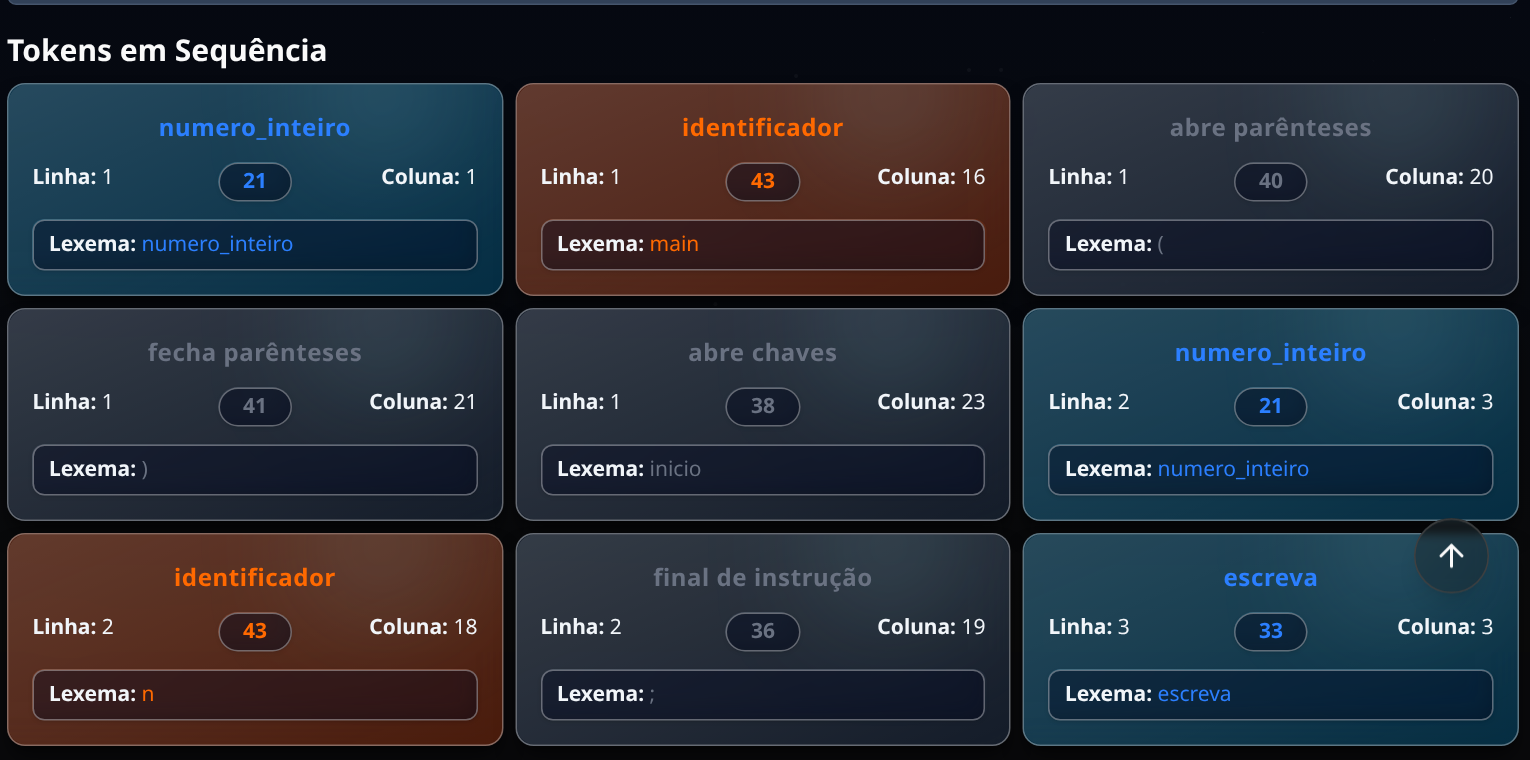
\includegraphics[width=\textwidth,height=0.36\textheight,keepaspectratio]{IDE/analise_lexica.png}
    \caption{Sequência de \textit{tokens} gerada para um programa escrito em Didática em Português.}
    \label{fig:ide-analise-lexica}
    \legend{Fonte: elaborado pelo autor.}
\end{figure}

\section{Execução do Código Intermediário e \textit{Feedback} no Terminal}
\label{sec:terminal-feedback}

O componente \texttt{terminal}, hospedado em \texttt{components/terminal}, foi modelado como o canal primário de \textit{feedback} interativo entre o programa em execução e o usuário. Sua arquitetura interna é composta por três peças: o componente \texttt{body}, que renderiza o histórico de saídas e o prompt de entrada; o componente \texttt{header}, que apresenta os controles de execução e o estado corrente; e o \textit{hook} \texttt{useKeyboardShortcuts}, que mapeia atalhos teclados às operações de limpeza, foco e interrupção da execução. O terminal é controlado pelo \texttt{TerminalContext}, responsável por gerenciar seu estado de abertura, fechamento e visibilidade na composição da tela.

A execução dos programas foi modelada de modo que as operações \texttt{print} e \texttt{scan} produzidas pelo interpretador sejam diretamente conectadas ao terminal embutido. O \texttt{Interpreter}, instanciado no navegador durante a execução interativa e no servidor Next.js durante a validação de submissões, recebe funções de retorno (\texttt{stdout} e \texttt{stdin}) cujo comportamento varia conforme o modo de execução: em modo interativo, as funções são associadas ao terminal da IDE; em modo de validação automatizada de exercícios, são conectadas a \textit{buffers} controlados que capturam a saída para comparação com o resultado esperado. Esse desacoplamento entre o motor de execução e a camada de apresentação atende aos princípios de baixo acoplamento discutidos por \citeonline{martin_clean} e foi inspirado nas abstrações de fluxos de entrada e saída descritas por \citeonline{cooper2012}.

Na depuração, a função \texttt{appendOutputLines} acumula os fragmentos de saída mantendo o estado da linha aberta. Fragmentos sem quebra de linha são concatenados, enquanto as sequências de fim de linha são normalizadas. Assim, a chegada de um novo fragmento durante um passo de execução não cria, por si só, uma linha adicional no terminal.

O núcleo compartilhado também passou a oferecer igualdade estrita (\texttt{===}) e expressão condicional ternária (\texttt{condicao ? valorA : valorB}). Incompatibilidades de atribuição e retorno podem gerar aviso na análise e erro durante a execução. A interface consome esses diagnósticos pelos mesmos canais de avisos e erros usados pelas demais construções. A igualdade estrita e os símbolos do ternário não integram os campos de operadores em forma de palavra do assistente atual.

No exemplo da Figura~\ref{fig:ide-execucao}, o programa escreve ``Digite um numero:'', recebe 7 pelo terminal, imprime \texttt{IMPAR} e o terminal registra o início e o fim da execução.

O sistema de \textit{feedback} de erros foi modelado em duas categorias complementares. Os erros estáticos detectados durante a compilação, como falhas léxicas, sintáticas e semânticas, são reportados pelo módulo \texttt{issue} do pacote \texttt{compiler}, que classifica cada ocorrência como \texttt{IssueError} (impede a tradução), \texttt{IssueWarning} (alerta não fatal) ou \texttt{IssueInfo} (informação contextual). Essas mensagens são interceptadas pela IDE e materializadas tanto no terminal, em formato textual, quanto no editor, por meio de marcadores de linha sublinhados, em conformidade com as práticas de relato de erros discutidas por \citeonline{aho1995}. Os erros dinâmicos, detectados pelo interpretador em tempo de execução (como divisões por zero, conversões impossíveis durante a leitura de entrada ou acessos a posições inválidas de \textit{arrays}), são encapsulados pela classe \texttt{RuntimeError} e gerenciados pelo \texttt{RuntimeErrorContext}, que coordena a exibição contextualizada no terminal e o destaque visual no editor.

Para garantir que mensagens de erro sejam pedagogicamente úteis, mesmo quando a linguagem corrente está fortemente personalizada, todas as mensagens passam pelo módulo de internacionalização \texttt{i18n} do pacote \texttt{compiler}, que oferece traduções para os idiomas \textit{pt-BR}, \textit{pt-PT}, \textit{es} e \textit{en}. Adicionalmente, as mensagens são adaptadas ao vocabulário corrente da customização: termos como ``palavra reservada esperada'' são substituídos pela palavra-chave efetivamente esperada na configuração ativa, evitando a exposição ao usuário de termos canônicos que tenham sido propositalmente ocultados pela personalização.

\section{Sistema de Correção e Avaliação Automatizada}
\label{sec:sistema-correcao}

A plataforma incorpora um subsistema de avaliação automatizada relacionado ao ciclo de submissão e veredito documentado pelo Beecrowd \cite{beecrowd2026faq}, materializado pela rota \texttt{/api/submissions/validate}. A modelagem do fluxo de submissão de exercícios partiu da estrutura conceitual desses juízes, mas foi adaptada ao contexto da linguagem dinâmica: enquanto os juízes tradicionais exigem que o aluno se adapte à sintaxe rígida de uma linguagem comercial, a plataforma proposta permite que cada exercício carregue sua própria configuração da linguagem, podendo, inclusive, restringir o aluno a um vocabulário específico definido pelo professor.


Entre as entidades persistidas estão \texttt{User}, \texttt{Class}, \texttt{Exercise}, \texttt{ExerciseList}, \texttt{Submission} e \texttt{Language}. A linguagem armazena a configuração do vocabulário e das variantes gramaticais; não se resume à imagem utilizada como identificação visual. Exercícios e listas podem definir uma política aberta ou vincular uma linguagem obrigatória, e a submissão registra uma cópia da configuração utilizada. O FastAPI e o SQLAlchemy mantêm esses registros, enquanto o \textit{TanStack React Query} gerencia consultas e atualização de dados na interface.

Na avaliação automática, a rota Next.js recebe código e configuração, normaliza as opções, executa a análise e gera as instruções intermediárias uma vez. Em seguida, consulta os casos de teste, executa cada caso com entrada simulada, coleta a saída e a compara à esperada após normalização de quebras de linha e remoção de espaços finais. A resposta reúne os vereditos; fora do modo de simulação, o resultado é encaminhado ao FastAPI para registro.

\subsection{Autoria de exercícios e acompanhamento de turmas}

A criação de exercícios envia enunciado, política de linguagem e casos de teste na mesma requisição. A edição completa usa \texttt{PUT /exercises/}\allowbreak\texttt{\{id\}}, substituindo também a coleção de casos de teste, que recebe índices de ordenação conforme a sequência enviada. O serviço verifica se o usuário é o professor responsável e valida a política de linguagem. A atualização parcial por \texttt{PATCH} continua disponível para os campos do exercício. Na interface, o diálogo de edição reúne os campos existentes, permite editar, acrescentar e remover casos de teste e atualiza as consultas após a gravação.

A listagem de turmas passou a devolver, além dos dados da turma, um resumo do professor e as contagens de membros e listas publicadas. Os cartões do painel utilizam esse contrato para apresentar o contexto da turma. Esses resumos são calculados a partir dos relacionamentos existentes e não acrescentam tabelas ao modelo de dados.

\subsection{Resolução de exercícios e linguagem obrigatória}

A área de resolução foi decomposta em componentes de cabeçalho, instruções, navegação da lista, painel de submissão e composição da IDE, no diretório \texttt{components/exercise-workspace}. O editor recebe um escopo de armazenamento por exercício e pode iniciar com o código da última submissão disponível. O cabeçalho distingue envio e reenvio, apresenta a nota existente e, quando há uma publicação com prazo vencido, substitui o botão de envio por uma indicação de prazo encerrado.

O painel de submissão separa erros de tradução, avisos e resultados dos casos de teste, incluindo quantos passaram e o total executado. A navegação lateral permite alternar entre os itens de uma lista e indicar as submissões disponíveis nesse contexto. Esses recursos dão continuidade ao trabalho no exercício, sem alterar a divisão entre execução local e avaliação no servidor.

Quando o exercício ou a lista exige uma linguagem, a API resolve a precedência entre a restrição do exercício, a da lista e o modo livre. O \texttt{KeywordContext} aplica a configuração recebida como uma sobreposição temporária, com nome, descrição e imagem da linguagem obrigatória. O seletor passa a apresentar apenas essa opção e bloqueia a troca; o estado temporário não é gravado como a preferência pessoal no armazenamento local. Ao encerrar a sobreposição, a configuração anterior é restaurada. O aviso de linguagem obrigatória identifica se a restrição veio do exercício ou da lista.

A Figura~\ref{fig:aluno-resultado} mostra a área de resolução depois de um envio. A faixa superior informa que a linguagem está travada pela lista e exibe o cartão da Didática em Português. O painel de submissão indica que um dos dois casos de teste passou; o caso que falhou está expandido, com a entrada 4, a saída esperada \texttt{PAR} e a saída obtida \texttt{IMPAR}. O erro vem do próprio programa enviado, que usa divisão (\texttt{n / 2}) onde deveria usar o resto (\texttt{n \% 2}).

\begin{figure}[htbp]
    \centering
    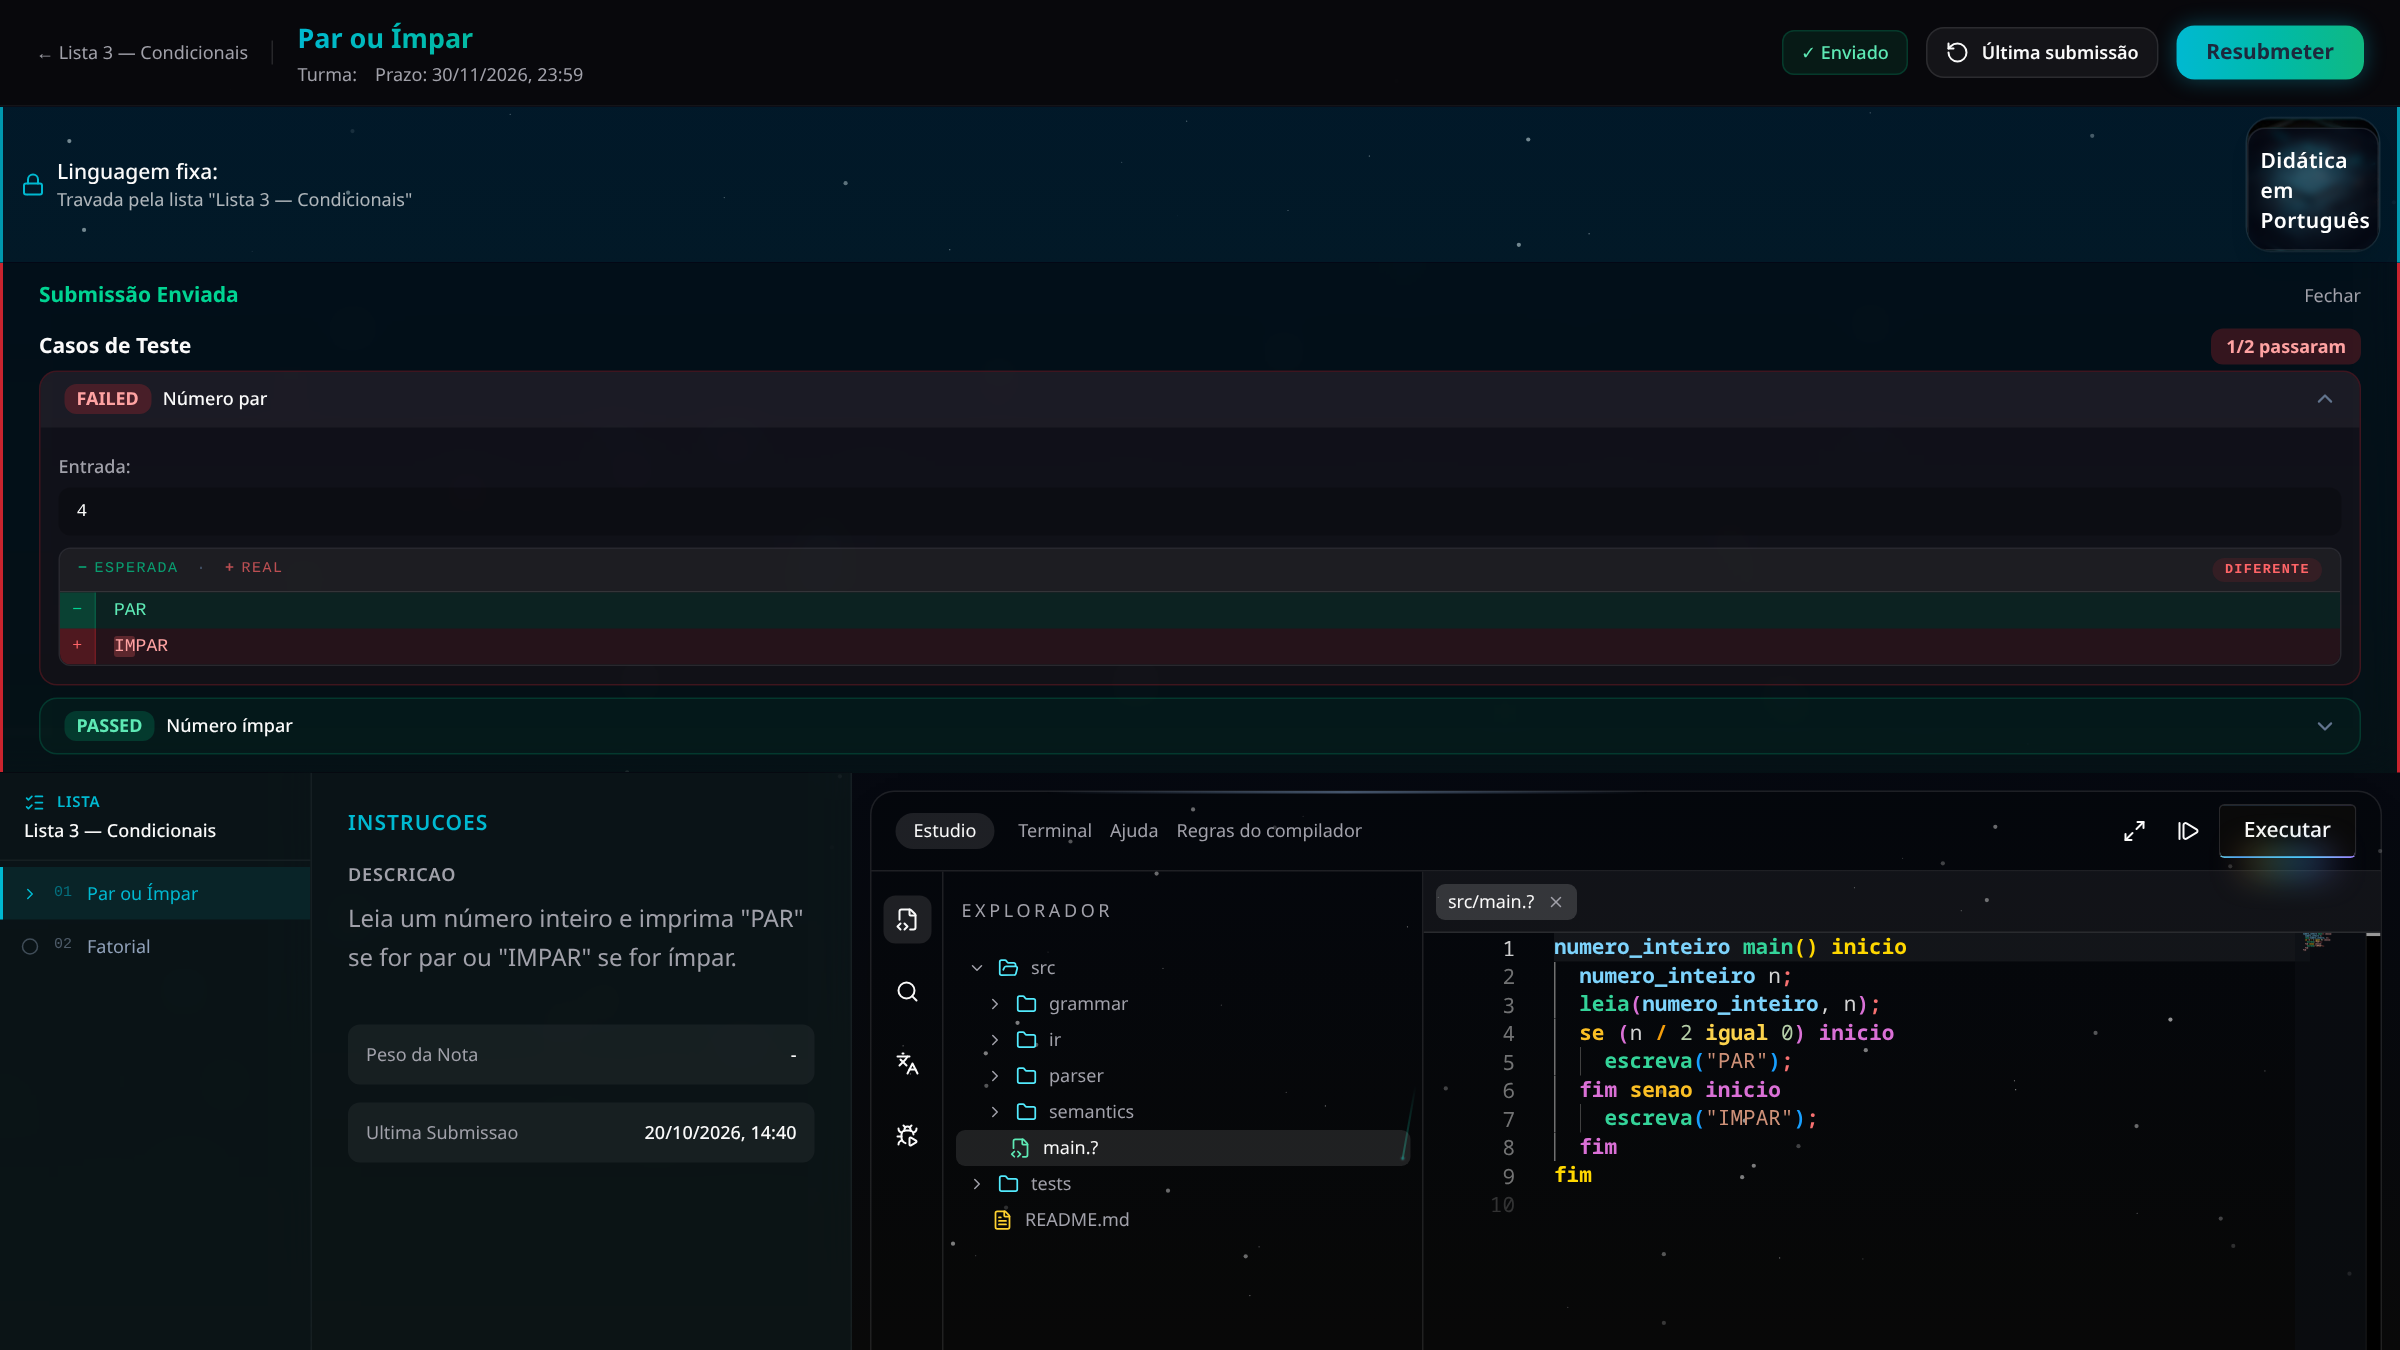
\includegraphics[width=\textwidth,height=0.42\textheight,keepaspectratio]{Aluno/resultado_submissao.png}
    \caption{Área de resolução após o envio, com linguagem obrigatória e resultado dos casos de teste.}
    \label{fig:aluno-resultado}
    \legend{Fonte: elaborado pelo autor.}
\end{figure}

\subsection{Correção de submissões pelo professor}
\label{subsec:correcao-professor}

A página de uma submissão, \texttt{/submissions/[id]}, reúne o enunciado e os casos de teste do exercício, o painel de nota e comentário e, abaixo deles, uma IDE completa carregada com a tentativa do aluno. O componente \texttt{SubmissionIdePanel} abre o editor com o código salvo em \texttt{code\_snapshot} e aplica a configuração de \texttt{language\_snapshot} como sobreposição temporária no \texttt{KeywordContext}, o mesmo mecanismo usado pela linguagem obrigatória. O professor lê e executa o programa no vocabulário que o aluno usou, sem trocar a própria linguagem ativa, que é restaurada ao sair da página. O editor usa um escopo de armazenamento próprio para cada submissão, e um botão devolve o código ao estado enviado depois de alterações feitas durante a correção.

Acima da IDE aparece o resultado de cada caso de teste registrado no envio: entrada, saída esperada, saída obtida e se o caso passou. Esses dados vêm do campo \texttt{test\_case\_results}, acrescentado à tabela de submissões em outubro. Antes dessa mudança, a rota de validação mostrava ao aluno o resultado de cada caso de teste, mas esses resultados não eram gravados, e o professor via apenas o estado e a nota da submissão. Os resultados mostrados são os da validação feita no envio; executar o código de novo na IDE da correção não os altera.

A Figura~\ref{fig:correcao-avaliacao} mostra a parte superior da mesma submissão aberta pelo professor. Nela ficam o enunciado, os casos de teste cadastrados, o painel de nota e comentário e o resultado registrado no envio, com a diferença entre a saída esperada e a obtida.

\begin{figure}[H]
    \centering
    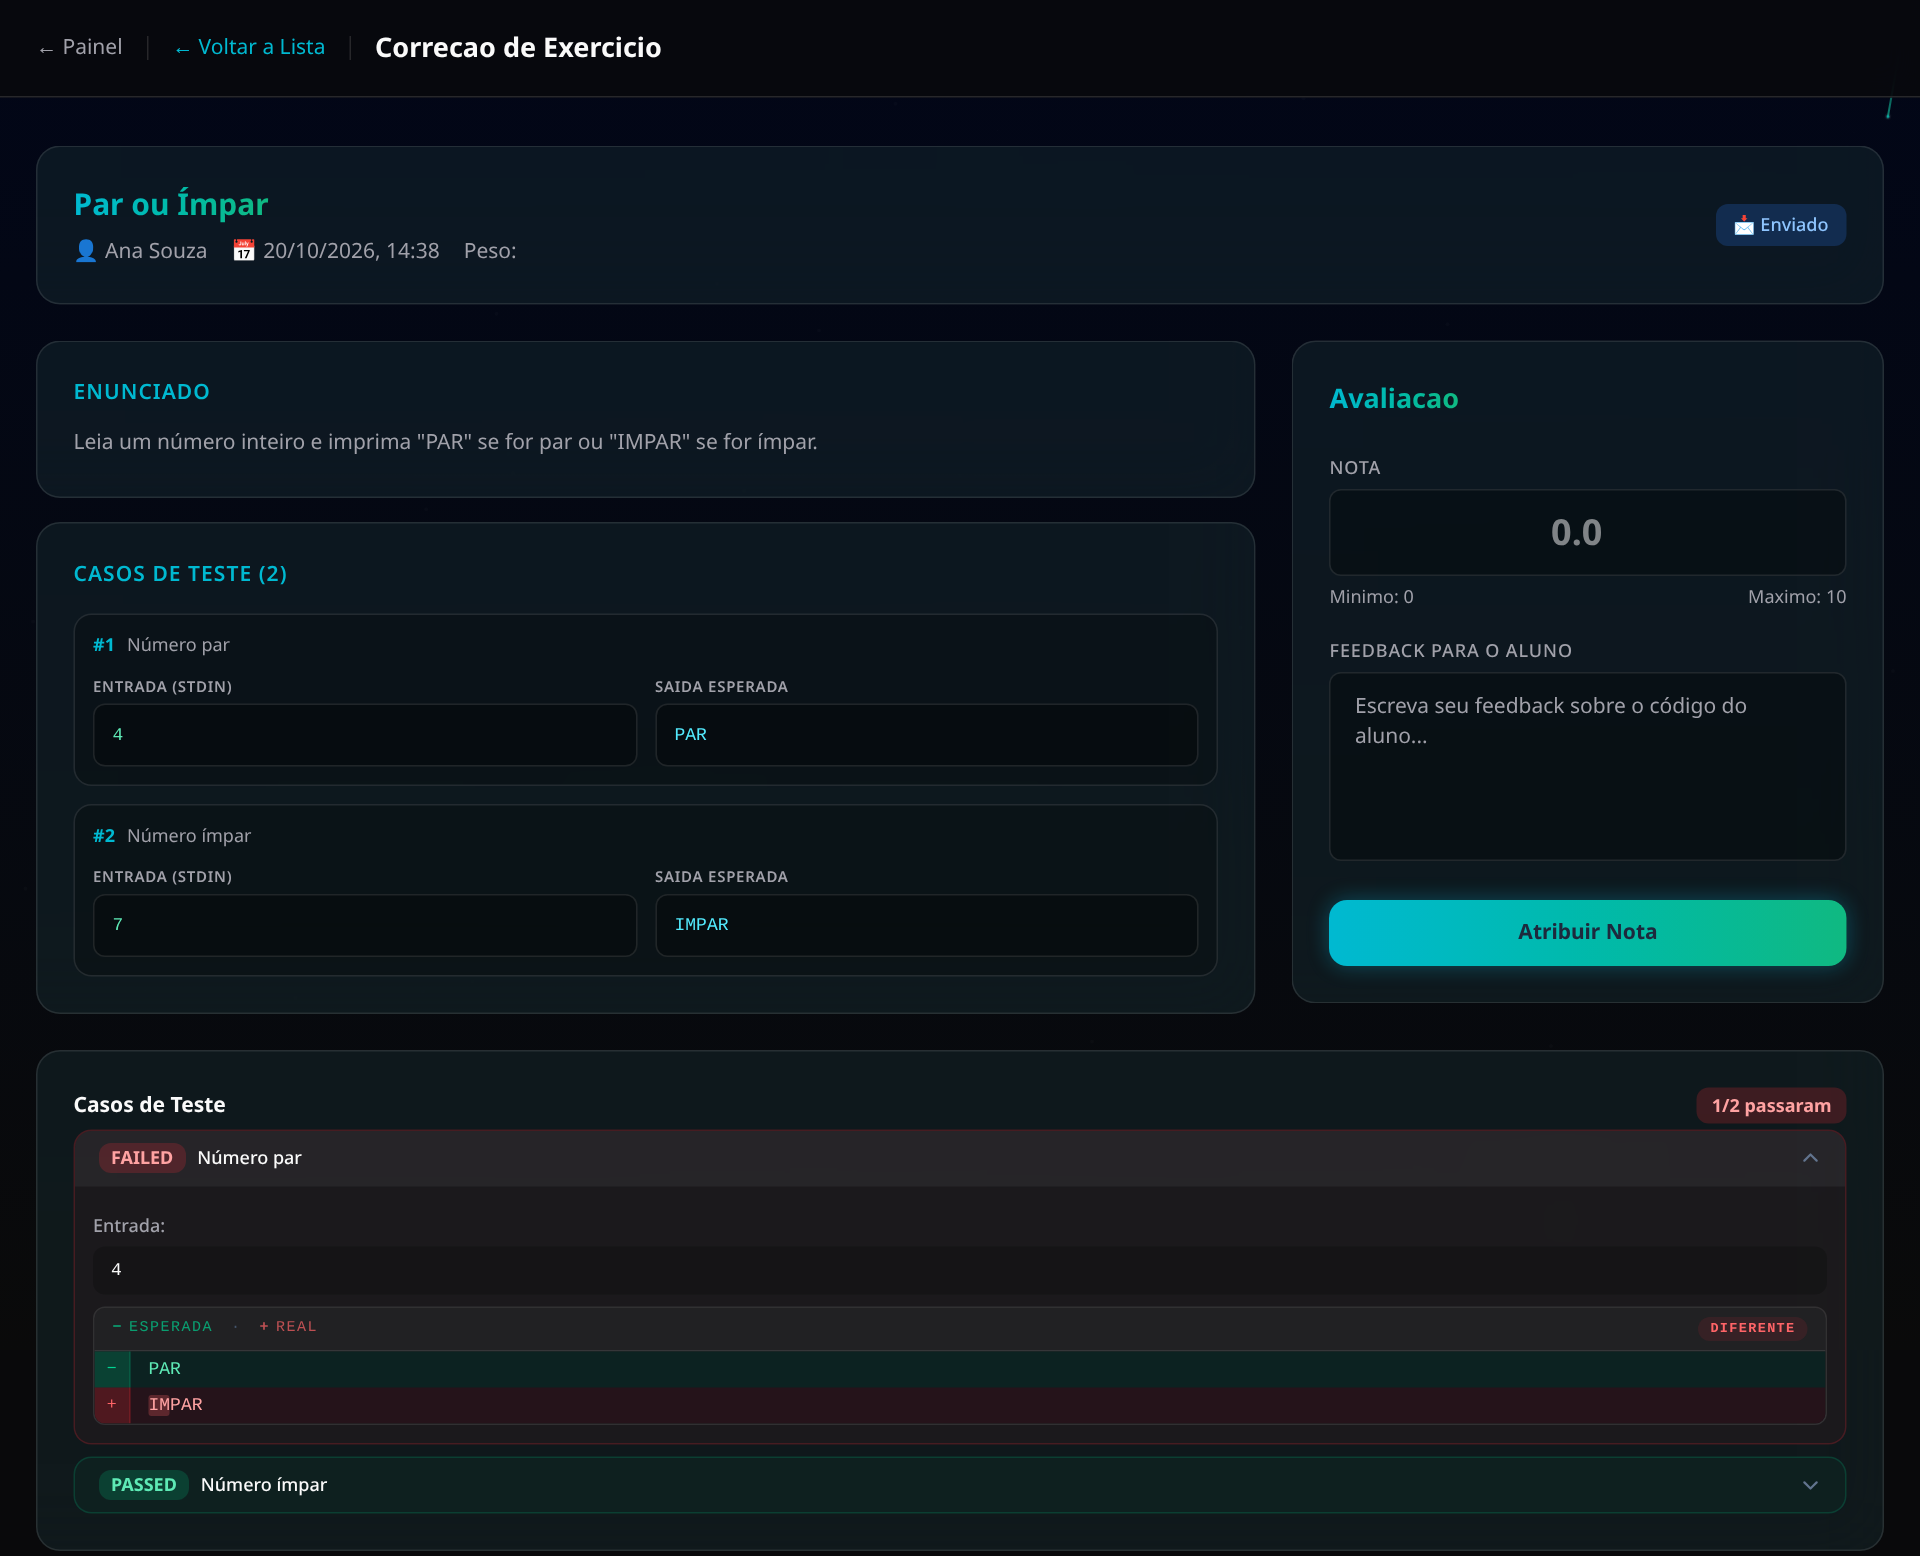
\includegraphics[width=\textwidth,height=0.34\textheight,keepaspectratio]{Professor/Correcao/avaliacao.png}
    \caption{Correção de uma submissão pelo professor: enunciado, casos de teste, avaliação e resultado registrado no envio.}
    \label{fig:correcao-avaliacao}
    \legend{Fonte: elaborado pelo autor.}
\end{figure}

Abaixo desse painel, a IDE abre com o código do aluno e com o destaque da linguagem usada no envio. Acima dela fica o botão que restaura o código enviado, como mostra a Figura~\ref{fig:correcao-ide}.

\begin{figure}[H]
    \centering
    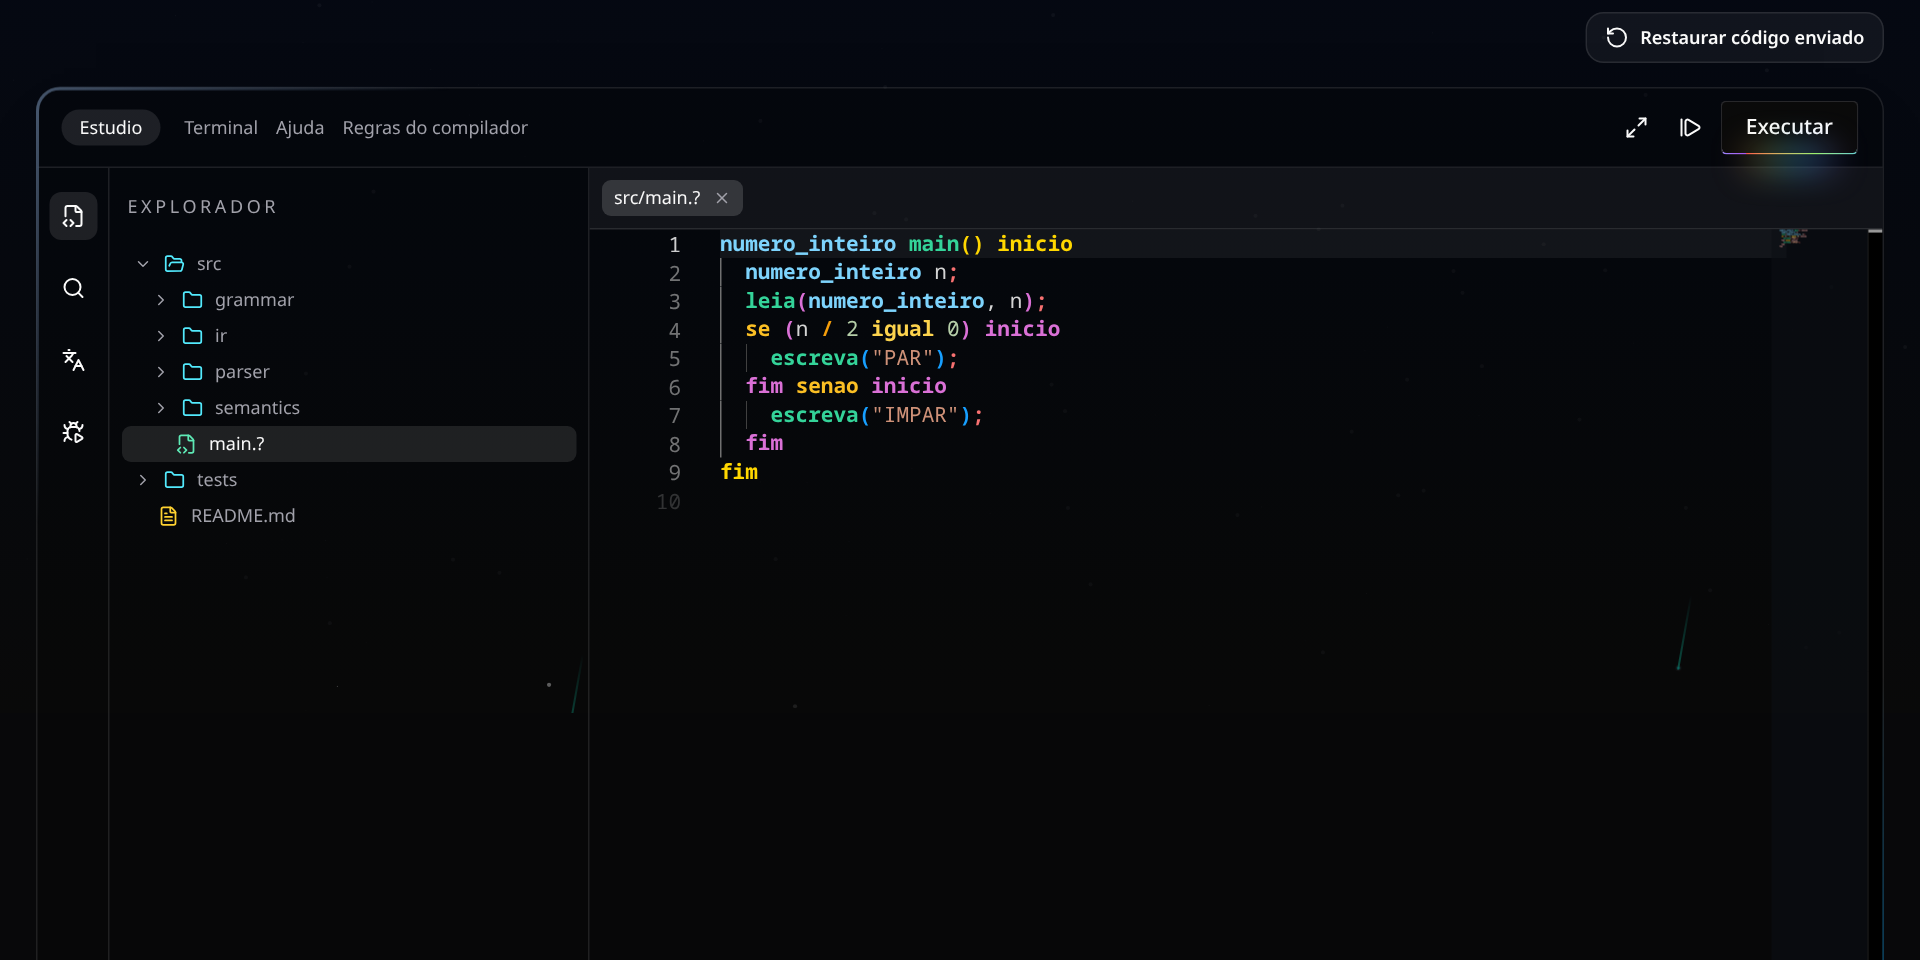
\includegraphics[width=\textwidth,height=0.34\textheight,keepaspectratio]{Professor/Correcao/ide.png}
    \caption{Correção de uma submissão pelo professor: IDE carregada com o código e a linguagem do envio.}
    \label{fig:correcao-ide}
    \legend{Fonte: elaborado pelo autor.}
\end{figure}

\section{Acessibilidade, Responsividade e Finalização de Fluxos}
\label{sec:acessibilidade-responsividade}

A acessibilidade foi examinada por inspeção de componentes e por uma verificação técnica delimitada, apresentada na Seção~\ref{subsec:verificacao-interface}. O módulo \texttt{ui/dialog.tsx} encapsula as primitivas de diálogo, título e descrição do Radix. O componente \texttt{WizardStepper} usa botões nativos e mantém os nomes das etapas com a classe \texttt{sr-only} quando os rótulos deixam de ser visíveis em telas estreitas. Entretanto, a indicação de etapa ativa nesse componente é visual, sem atributo \texttt{aria-current}. Essas evidências mostram recursos e lacunas da implementação; não permitem declarar conformidade global com WAI-ARIA ou WCAG.

A adaptação visual usa utilidades responsivas do Tailwind CSS. No assistente, abaixo do limite \texttt{lg}, a lista de etapas assume disposição horizontal, os botões tornam-se circulares e o cartão da linguagem-base é ocultado. Acima desse limite, as etapas ficam na lateral. O \textit{hook} \texttt{useBreakpoint} também disponibiliza consultas por largura. Na IDE, a composição usa \texttt{flex-col} e \texttt{sm:flex-row} para reorganizar os painéis.


Os temas claro e escuro são administrados pelo \texttt{ThemeContext}, que aplica a classe \texttt{dark} e persiste a preferência no navegador, com alternância dos temas do Monaco. As Figuras~\ref{fig:home-light} e \ref{fig:home-dark} ilustram essa escolha. As notificações são centralizadas no \texttt{ToastContext}.

\subsection{Internacionalização da interface}
\label{subsec:internacionalizacao}

O requisito RNF03 pede que toda cadeia visível ao usuário esteja externalizada, com suporte a \textit{pt-BR}, \textit{pt-PT}, \textit{es} e \textit{en}. A configuração do Next.js declara esses quatro locais, e os textos ficam no diretório \texttt{i18n/locales}, com um subdiretório por idioma. Cada idioma tem oito arquivos, separados por área da aplicação: \texttt{ui}, \texttt{wizard}, \texttt{toast}, \texttt{ide}, \texttt{footer}, \texttt{language-documentation}, \texttt{language-sample} e \texttt{compiler-rules}. Em \textit{pt-BR}, somam 1.690 linhas.

Os componentes obtêm o texto de duas formas. A maioria chama a função \texttt{t}, exportada por \texttt{i18n}, passando o local corrente e a chave desejada. O assistente de personalização usa o \textit{hook} \texttt{useWizardTranslation}, que lê o local pelo roteador do Next.js e acrescenta o prefixo \texttt{wizard.} às chaves, evitando repetir esse prefixo em cada etapa. As mensagens de erro do compilador seguem caminho próprio, descrito na Seção~\ref{sec:terminal-feedback}: são traduzidas pelo módulo \texttt{i18n} do pacote \texttt{compiler} e adaptadas ao vocabulário da linguagem ativa.

Dois conteúdos didáticos acompanham o idioma escolhido. O primeiro são os arquivos iniciais da IDE, declarados em \texttt{defaultFiles.ts}: a área de trabalho não começa vazia, mas com uma árvore que reproduz a estrutura de um tradutor, em que cada arquivo traz um texto comentado sobre a fase correspondente. Ao trocar de idioma esses arquivos são reescritos, com uma exceção: o arquivo do programa do próprio estudante é preservado, para que a troca não descarte o trabalho já feito. O segundo é a amostra de linguagem exibida no painel lateral, montada pela função \texttt{buildHelloWorldSample} a partir da personalização ativa; os identificadores e as cadeias do exemplo também vêm do pacote de idioma, de modo que um exemplo em português não apresente nomes de variáveis em inglês.

A cobertura, porém, é parcial. Os componentes foram contados como os arquivos \texttt{.tsx} de \texttt{components}, \texttt{views} e \texttt{pages} que importam \texttt{i18n}. Na revisão de 22 de setembro, 56 dos 180 componentes da interface usavam o mecanismo de tradução. Na versão de 19 de outubro, contados da mesma forma, são 98 de 187. O total de componentes aumentou de 180 para 187 porque a interface ganhou sete arquivos entre as duas versões, e nenhum foi removido: os dois componentes dos tutoriais, a página Sobre, o diálogo de regras do compilador e o painel da IDE na correção de submissões, descritos na Seção~\ref{sec:orientacao-usuario} e na Subseção~\ref{subsec:correcao-professor}, e dois componentes visuais de \texttt{components/ui}. Nesse intervalo passaram a ser traduzidos as listas e o catálogo de exercícios, as telas de submissão e de linguagens, o cadastro e a entrada no sistema. Continuam com cadeias fixas a área de resolução de exercícios, o aviso de linguagem obrigatória e o painel de resultados dos casos de teste. Em \texttt{components/exercise-workspace}, por exemplo, a mensagem ``Submissão enviada com sucesso!'' ainda está escrita em português no código. Boa parte dos 89 componentes restantes não exibe texto ao usuário, como as primitivas de \texttt{components/ui} e os fundos animados, de modo que a contagem não mede diretamente quanto texto falta traduzir. O requisito RNF03 ainda não pode ser considerado cumprido.

O \texttt{AuthContext} recupera o perfil autenticado e o utilitário \texttt{auth-cookies} mantém o token em um \textit{cookie} acessível por JavaScript. A interface distingue os papéis administrador, professor, aluno e comunidade, e o modelo de dados inclui ainda um papel interno de sistema.

\section{Recursos de Orientação ao Usuário}
\label{sec:orientacao-usuario}

A revisão de outubro acrescentou recursos que explicam a plataforma a quem a usa pela primeira vez: tutoriais guiados, um diálogo com um exemplo da linguagem ativa, um diálogo com as regras do compilador e uma página sobre o projeto. Nenhum deles altera a linguagem configurada ou a execução dos programas.

\subsection{Tutoriais guiados}
\label{subsec:tutoriais}

Os tutoriais usam a biblioteca \textit{React Joyride} e estão declarados em \texttt{lib/tutorials.ts}. São cinco roteiros, cada um ligado a uma tela: a IDE, com nove passos; o assistente de criação de linguagem, com quatro; a criação de exercícios, com cinco; e os painéis do professor e do aluno, com três e dois passos. Cada passo aponta para um elemento marcado com o atributo \texttt{data-tour}, e o título e o texto de cada passo vêm dos arquivos de idioma, nos quatro locais.

O tutorial não abre sozinho. O rodapé mostra um botão de ajuda quando a rota corrente tem um roteiro associado, e o roteiro começa quando o usuário clica nele. A escolha depende também do perfil: em \texttt{/exercises} o roteiro só aparece para professores, e em \texttt{/dashboard} professor e aluno recebem roteiros diferentes. Durante o tutorial, a tecla \texttt{Enter} avança e \texttt{Esc} encerra. Se o elemento de um passo não estiver na tela, o passo é pulado.

O roteiro do assistente de criação de linguagem tem quatro passos, mostrados nas Figuras~\ref{fig:tutorial-linguagem-1} a~\ref{fig:tutorial-linguagem-4}. Em cada passo, o restante da tela fica escurecido e o elemento indicado aparece destacado, ao lado de um balão com o número do passo, uma barra de progresso, o título e o texto. O balão tem os botões ``Pular'' e ``Proximo''; ``Voltar'' aparece a partir do segundo passo, e no último passo ``Proximo'' dá lugar a ``Concluir''. Os textos em português aparecem sem acentos, como em ``criacao'' e ``Proximo'', porque estão gravados assim no arquivo de idioma \texttt{pt-BR}.

O primeiro passo aponta para a lista das sete etapas do assistente, como mostra a Figura~\ref{fig:tutorial-linguagem-1}.

\begin{figure}[H]
    \centering
    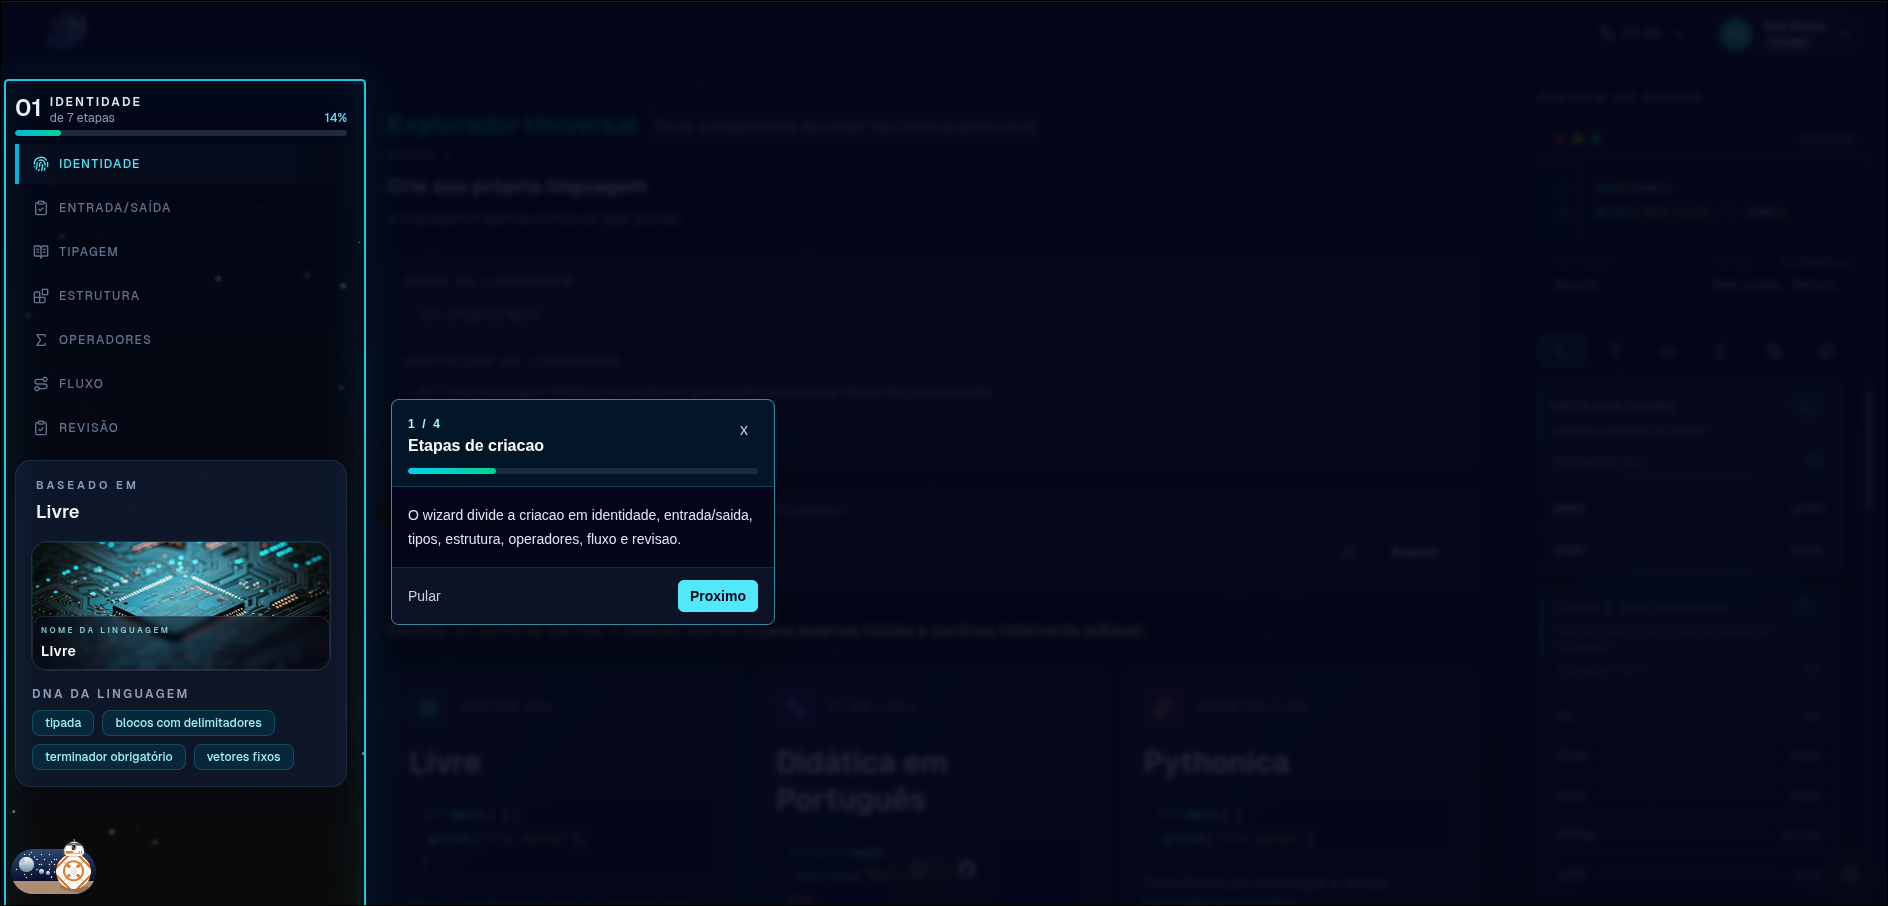
\includegraphics[width=\textwidth,height=0.34\textheight,keepaspectratio]{Tutoriais/criacao_linguagem_1.png}
    \caption{Passo 1 do tutorial do assistente de criação de linguagem: etapas de criação.}
    \label{fig:tutorial-linguagem-1}
    \legend{Fonte: elaborado pelo autor.}
\end{figure}

O segundo passo aponta para o formulário da etapa corrente (Figura~\ref{fig:tutorial-linguagem-2}).

\begin{figure}[H]
    \centering
    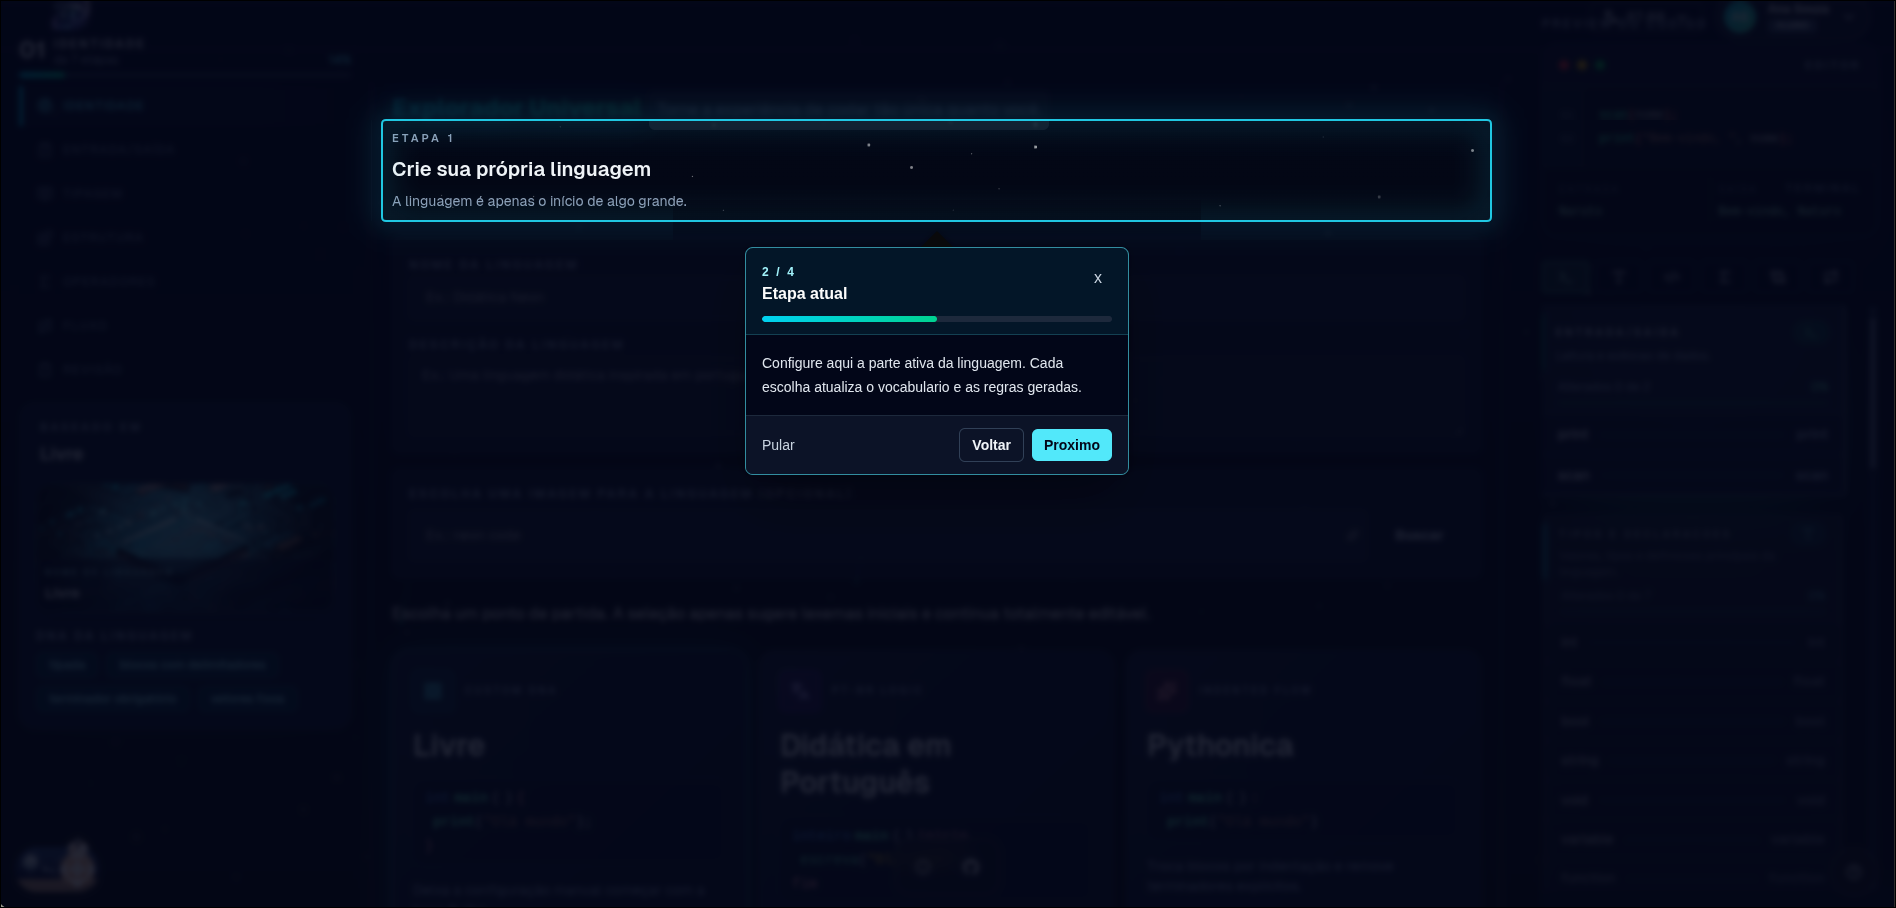
\includegraphics[width=\textwidth,height=0.34\textheight,keepaspectratio]{Tutoriais/criacao_linguagem_2.png}
    \caption{Passo 2 do tutorial do assistente de criação de linguagem: etapa atual.}
    \label{fig:tutorial-linguagem-2}
    \legend{Fonte: elaborado pelo autor.}
\end{figure}

O terceiro passo aponta para a prévia do código, que muda a cada alteração feita no formulário (Figura~\ref{fig:tutorial-linguagem-3}).

\begin{figure}[H]
    \centering
    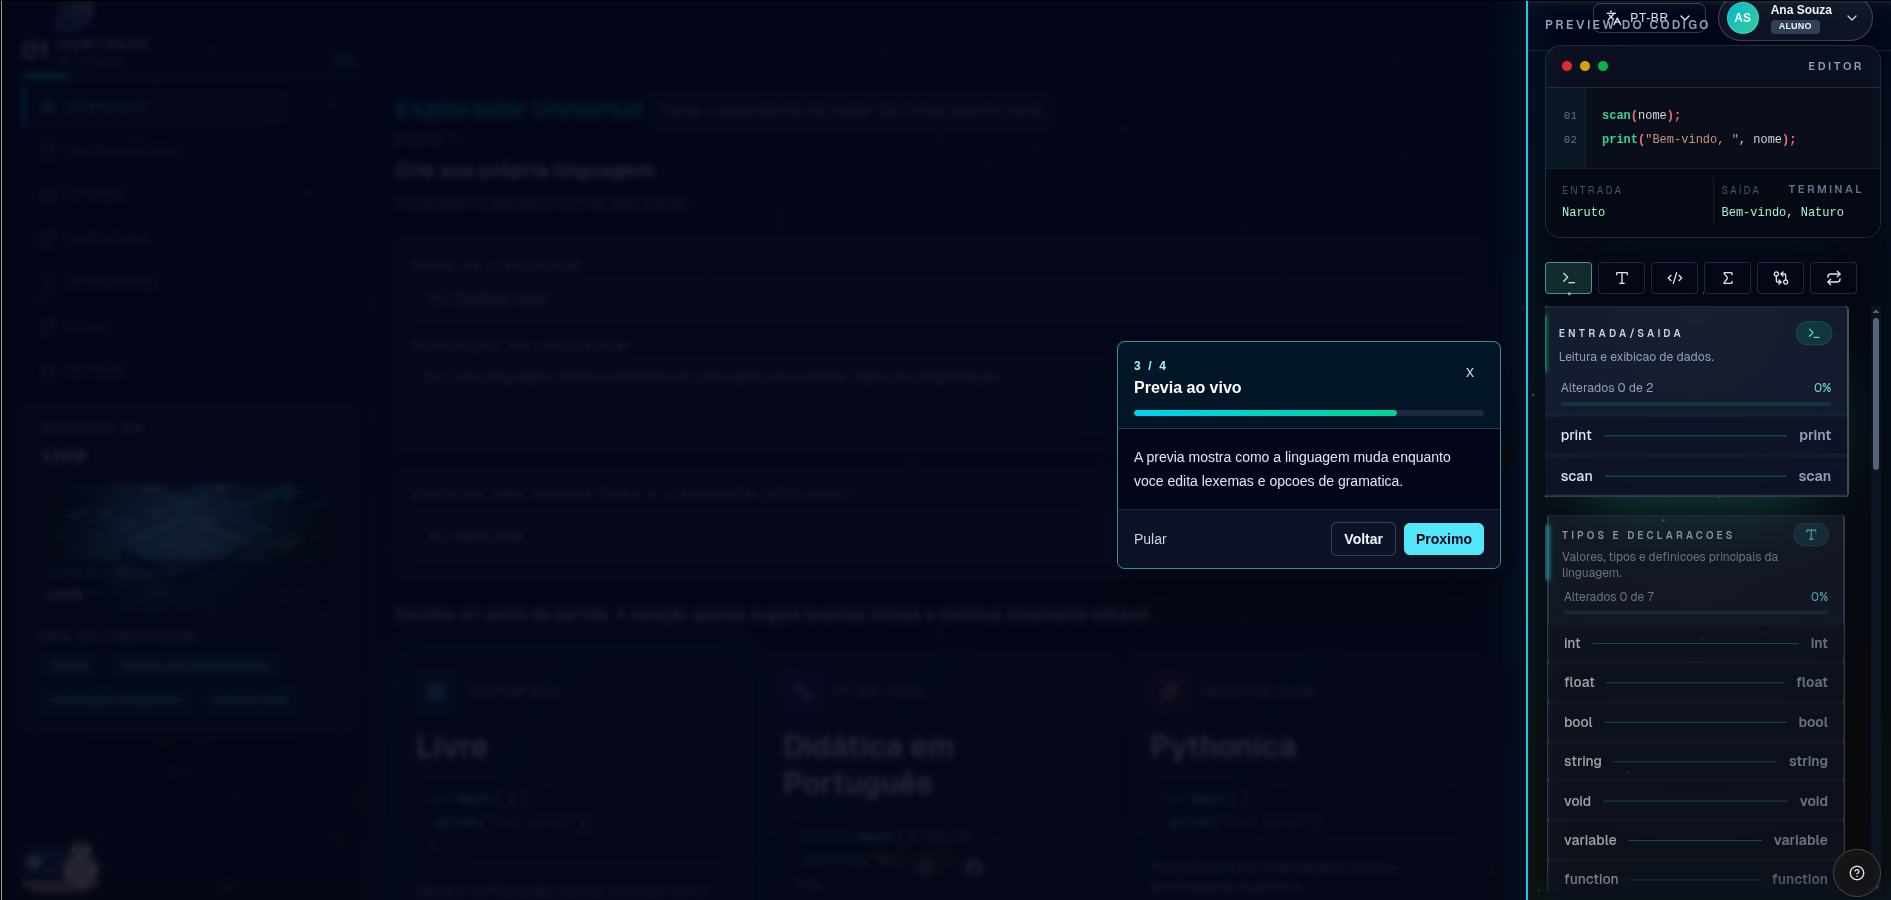
\includegraphics[width=\textwidth,height=0.34\textheight,keepaspectratio]{Tutoriais/criacao_linguagem_3.png}
    \caption{Passo 3 do tutorial do assistente de criação de linguagem: prévia ao vivo.}
    \label{fig:tutorial-linguagem-3}
    \legend{Fonte: elaborado pelo autor.}
\end{figure}

O quarto e último passo aponta para o rodapé com os botões de navegação do assistente, por onde o usuário avança, volta e salva a linguagem (Figura~\ref{fig:tutorial-linguagem-4}).

\begin{figure}[H]
    \centering
    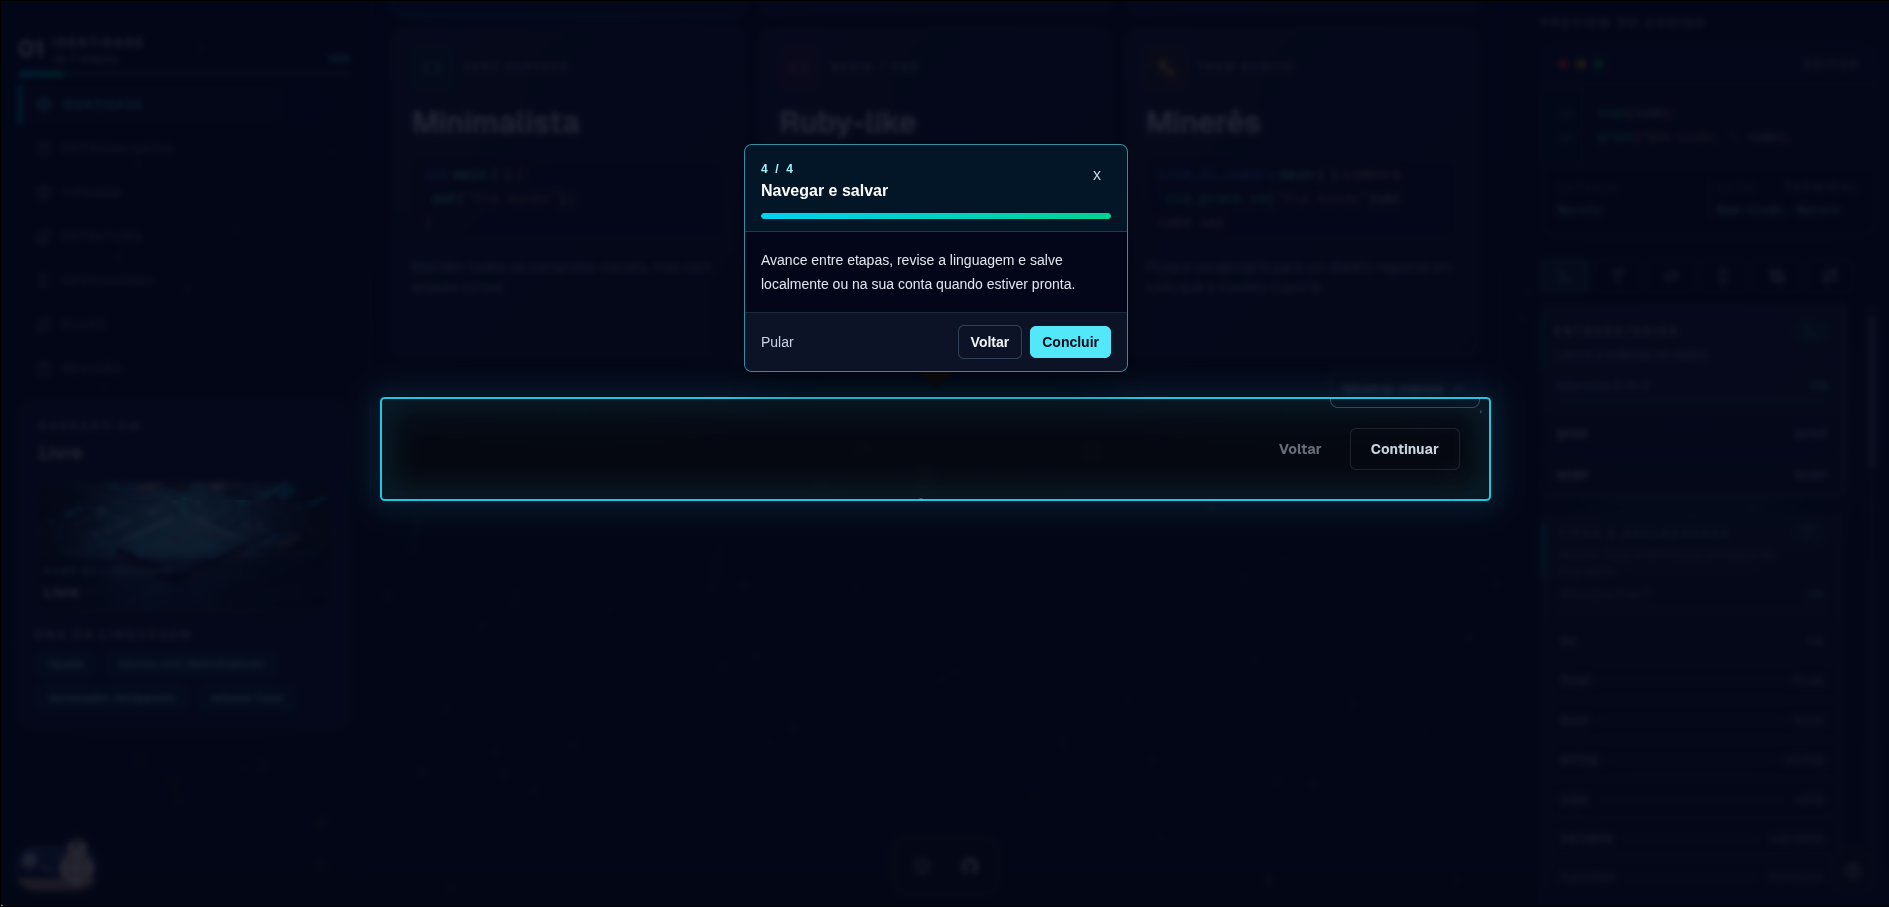
\includegraphics[width=\textwidth,height=0.34\textheight,keepaspectratio]{Tutoriais/criacao_linguagem_4.png}
    \caption{Passo 4 do tutorial do assistente de criação de linguagem: navegar e salvar.}
    \label{fig:tutorial-linguagem-4}
    \legend{Fonte: elaborado pelo autor.}
\end{figure}

Ao terminar ou pular um roteiro, a conclusão é gravada no armazenamento local do navegador, em uma chave com o prefixo \texttt{di:tutorial:}.

\subsection{Exemplo da linguagem e regras do compilador}
\label{subsec:regras-compilador}

O menu da IDE ganhou dois botões ao lado do botão do terminal: Ajuda e Regras do compilador. Os três ficam ocultos em telas mais estreitas que o limite \texttt{md} do Tailwind CSS. Ajuda abre um diálogo com o exemplo da linguagem ativa, montado com os lexemas da personalização corrente, o mesmo exemplo descrito na Subseção~\ref{subsec:internacionalizacao}. Pelo diálogo, o usuário pode substituir o arquivo selecionado no editor por esse código.

Regras do compilador abre um diálogo com sete grupos de regras: formato do programa; blocos e finais de instrução; entrada, saída e atualizações; modo tipado; arranjos; literais de arranjo; e modo sem tipo. Os textos e os trechos de código vêm do arquivo \texttt{compiler-rules} de cada idioma e usam sempre as palavras canônicas, como \texttt{int}, \texttt{print} e \texttt{if}, qualquer que seja a linguagem ativa. Um estudante que configurou \texttt{escreva} no lugar de \texttt{print} lê a regra escrita com \texttt{print}. O pacote \texttt{compiler} tem um resumo próprio das regras, em \texttt{language-rules.ts}, que o diálogo não usa; o texto complementar registra essa duplicação.

Os dois diálogos foram capturados na IDE de correção, com a Didática em Português aplicada. No diálogo de ajuda, o exemplo da linguagem usa \texttt{numero\_inteiro}, \texttt{se}, \texttt{inicio} e \texttt{fim} (Figura~\ref{fig:dialogo-ajuda}).

\begin{figure}[H]
    \centering
    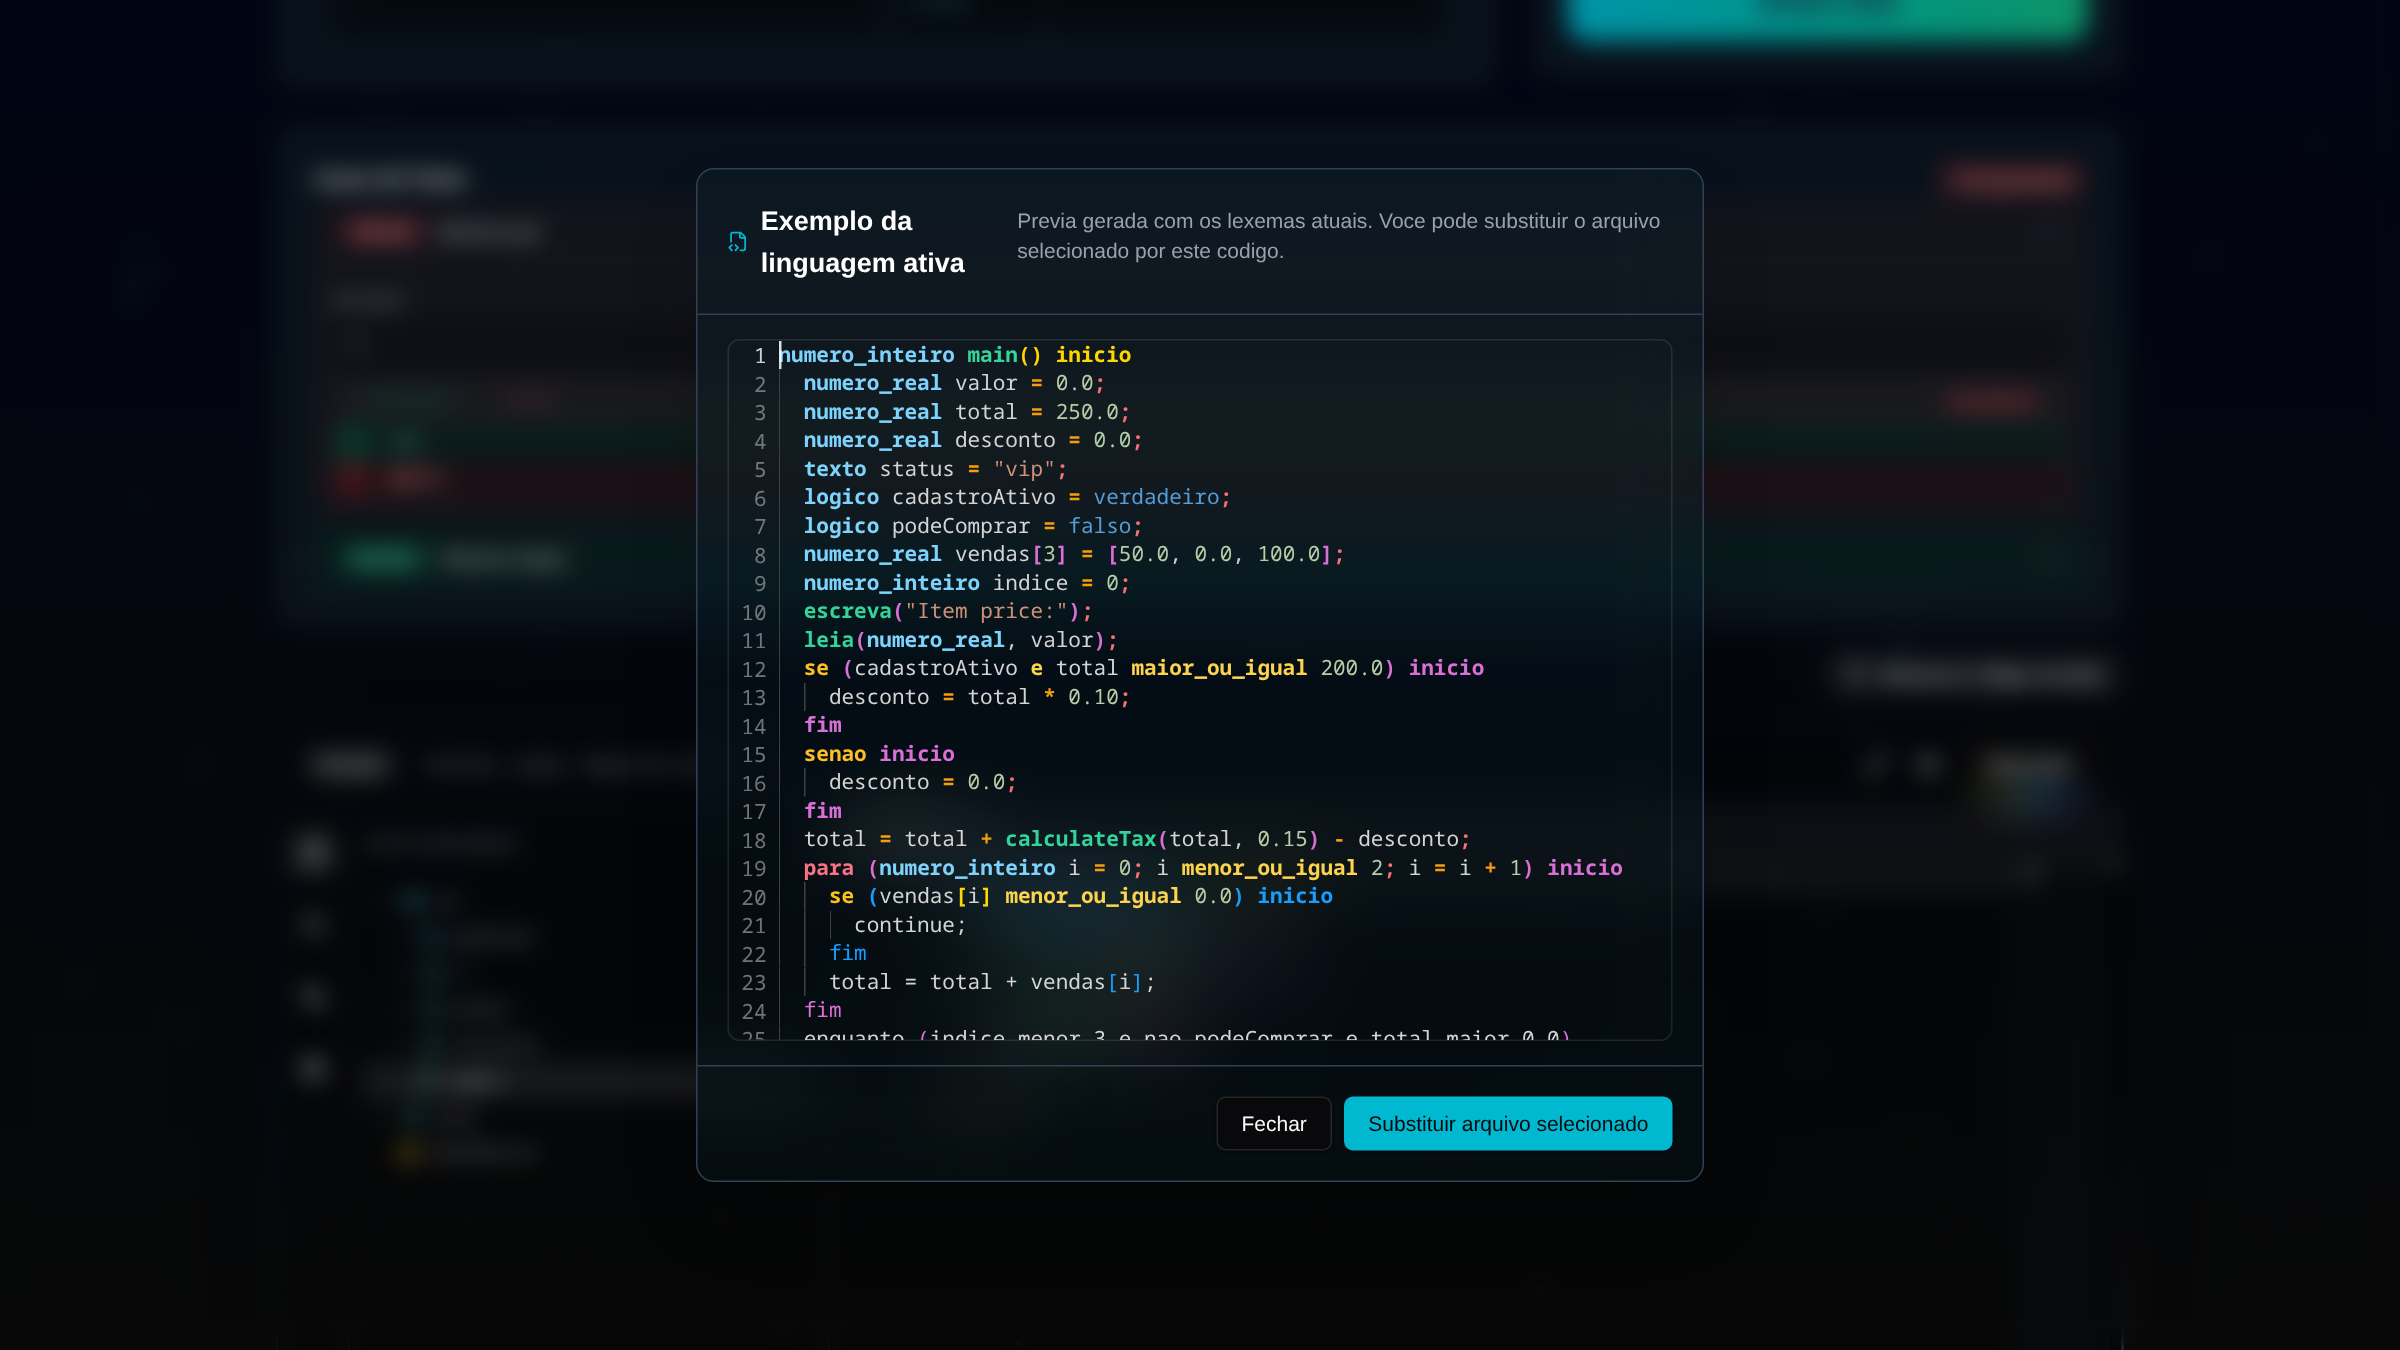
\includegraphics[width=\textwidth,height=0.34\textheight,keepaspectratio]{IDE/ajuda_exemplo.png}
    \caption{Diálogo de ajuda da IDE com o exemplo da linguagem Didática em Português.}
    \label{fig:dialogo-ajuda}
    \legend{Fonte: elaborado pelo autor.}
\end{figure}

O diálogo de regras, aberto na mesma tela, apresenta os trechos com \texttt{int}, \texttt{print}, \texttt{if} e chaves, e não com as palavras da linguagem ativa (Figura~\ref{fig:dialogo-regras}).

\begin{figure}[H]
    \centering
    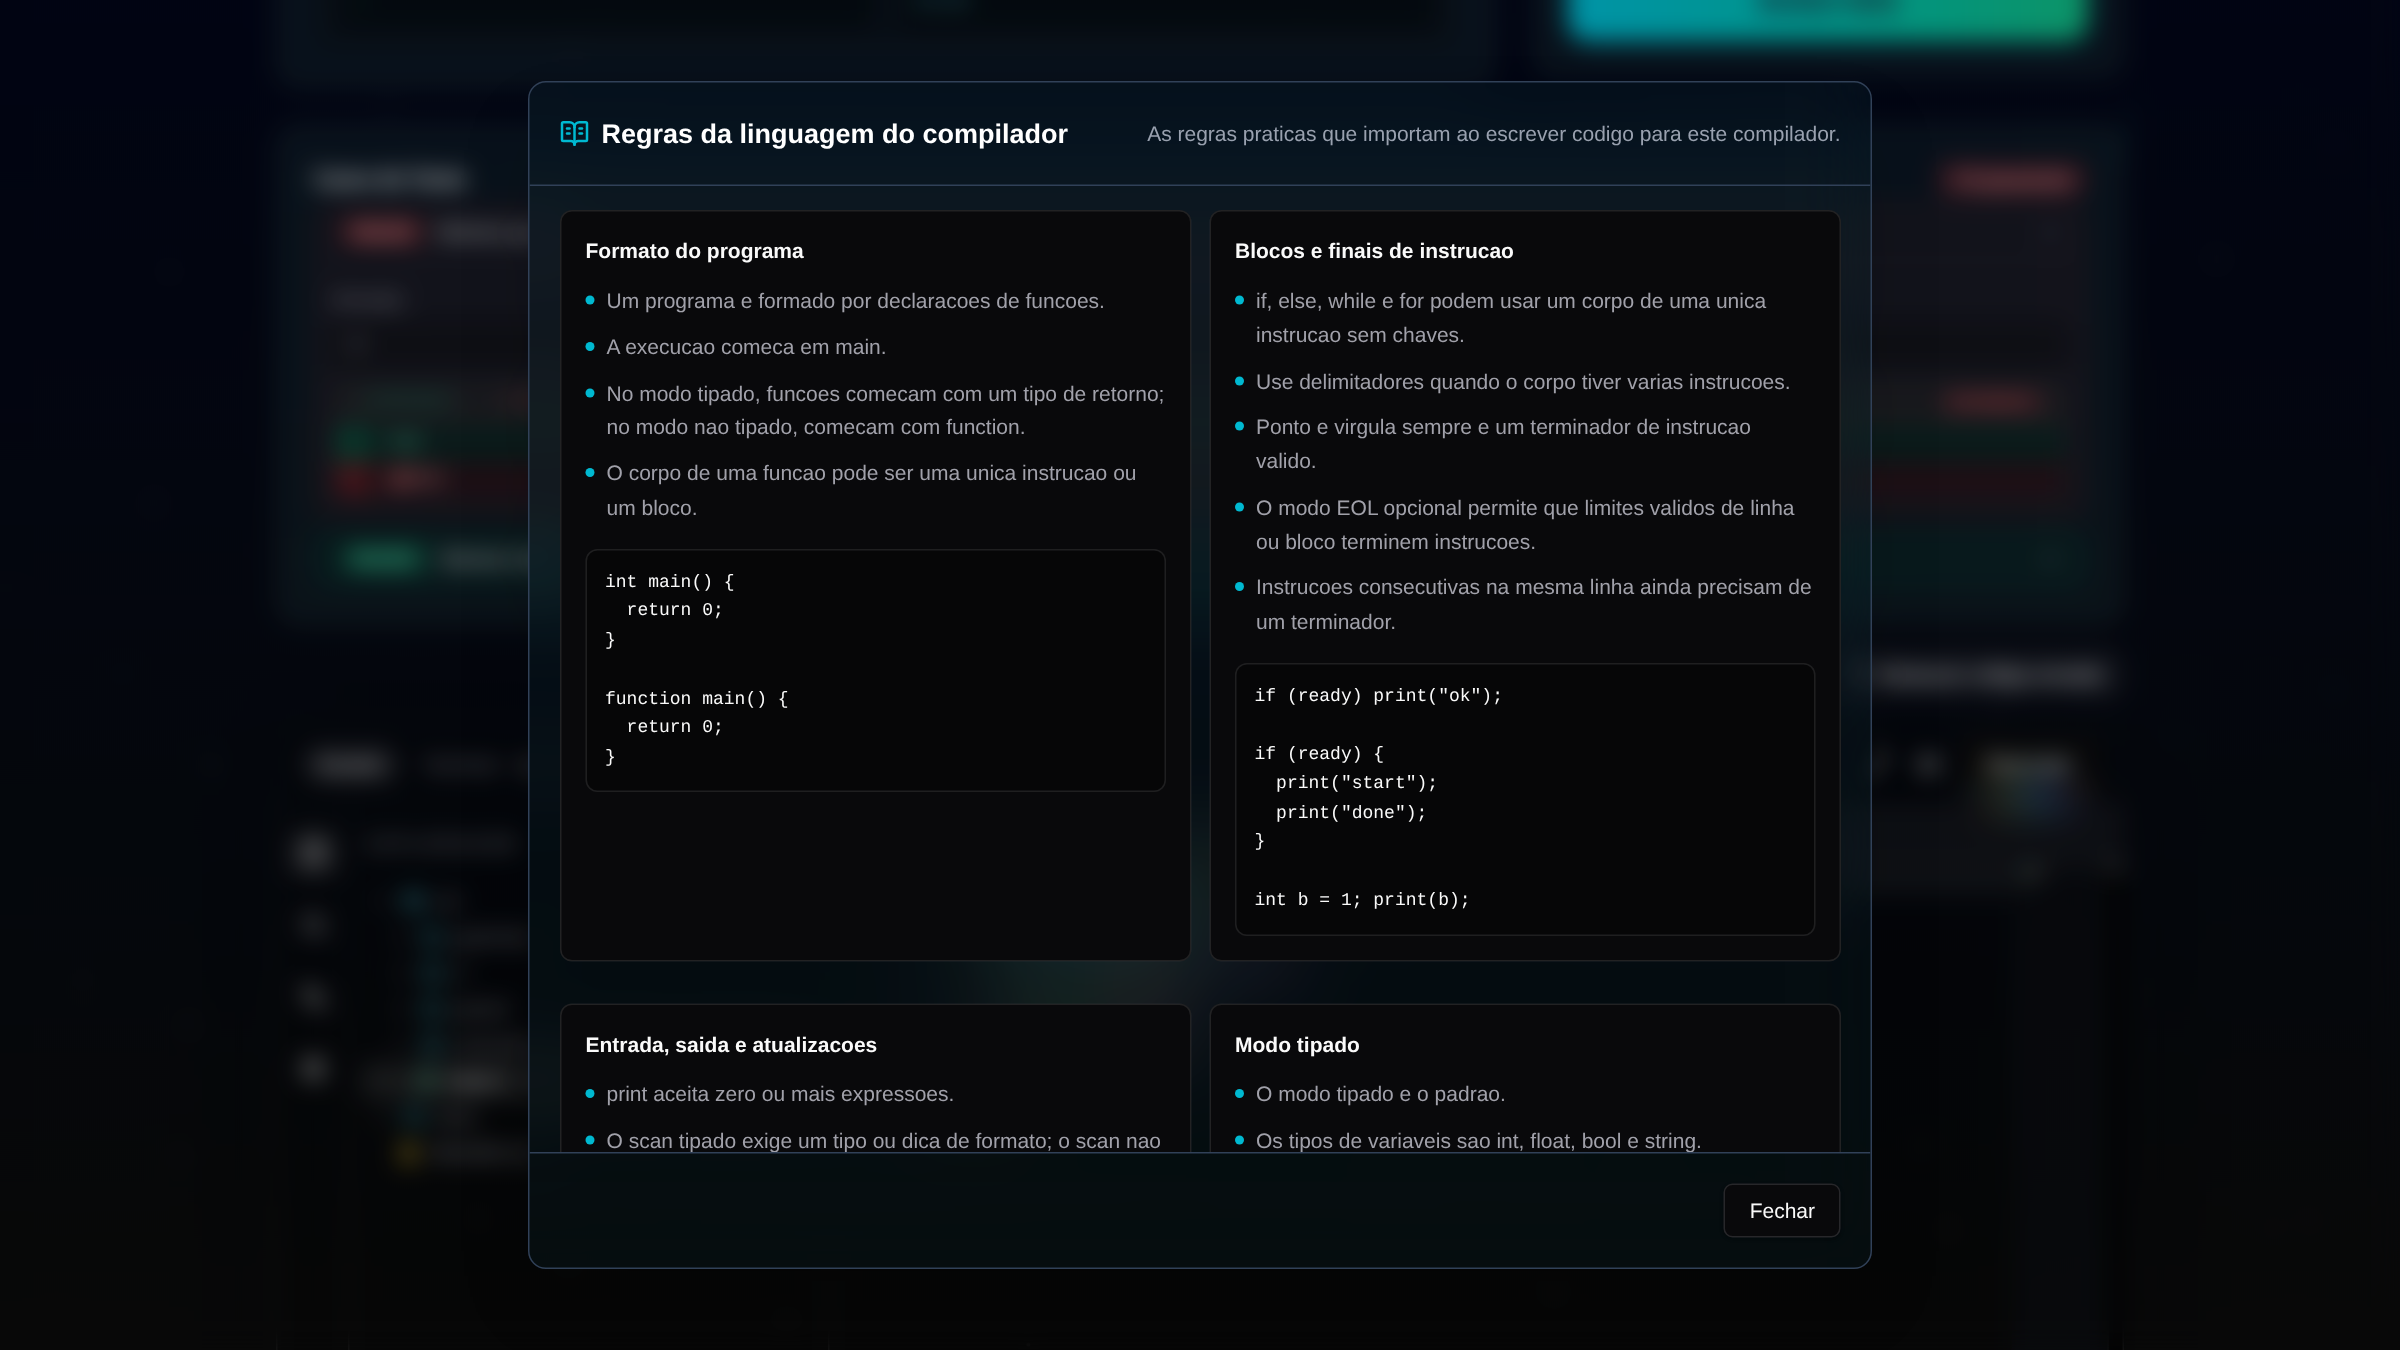
\includegraphics[width=\textwidth,height=0.34\textheight,keepaspectratio]{IDE/regras_compilador.png}
    \caption{Diálogo de regras do compilador aberto com a linguagem Didática em Português ativa.}
    \label{fig:dialogo-regras}
    \legend{Fonte: elaborado pelo autor.}
\end{figure}

\subsection{Página Sobre}
\label{subsec:pagina-sobre}

A página \texttt{/about}, aberta pelo ícone de informação do rodapé, apresenta o projeto como trabalho de conclusão de curso. Ela traz os autores, a área, quatro destaques da plataforma e uma galeria com quatro capturas de tela: a IDE, o painel de \textit{tokens}, a criação de linguagem e o painel do professor. Como as demais telas novas, a página obtém seus textos dos arquivos de idioma.



A Figura~\ref{fig:pagina-sobre} mostra a parte inicial da página, com o título do projeto, a descrição, os autores, a área e a primeira imagem da galeria.

\begin{figure}[htbp]
    \centering
    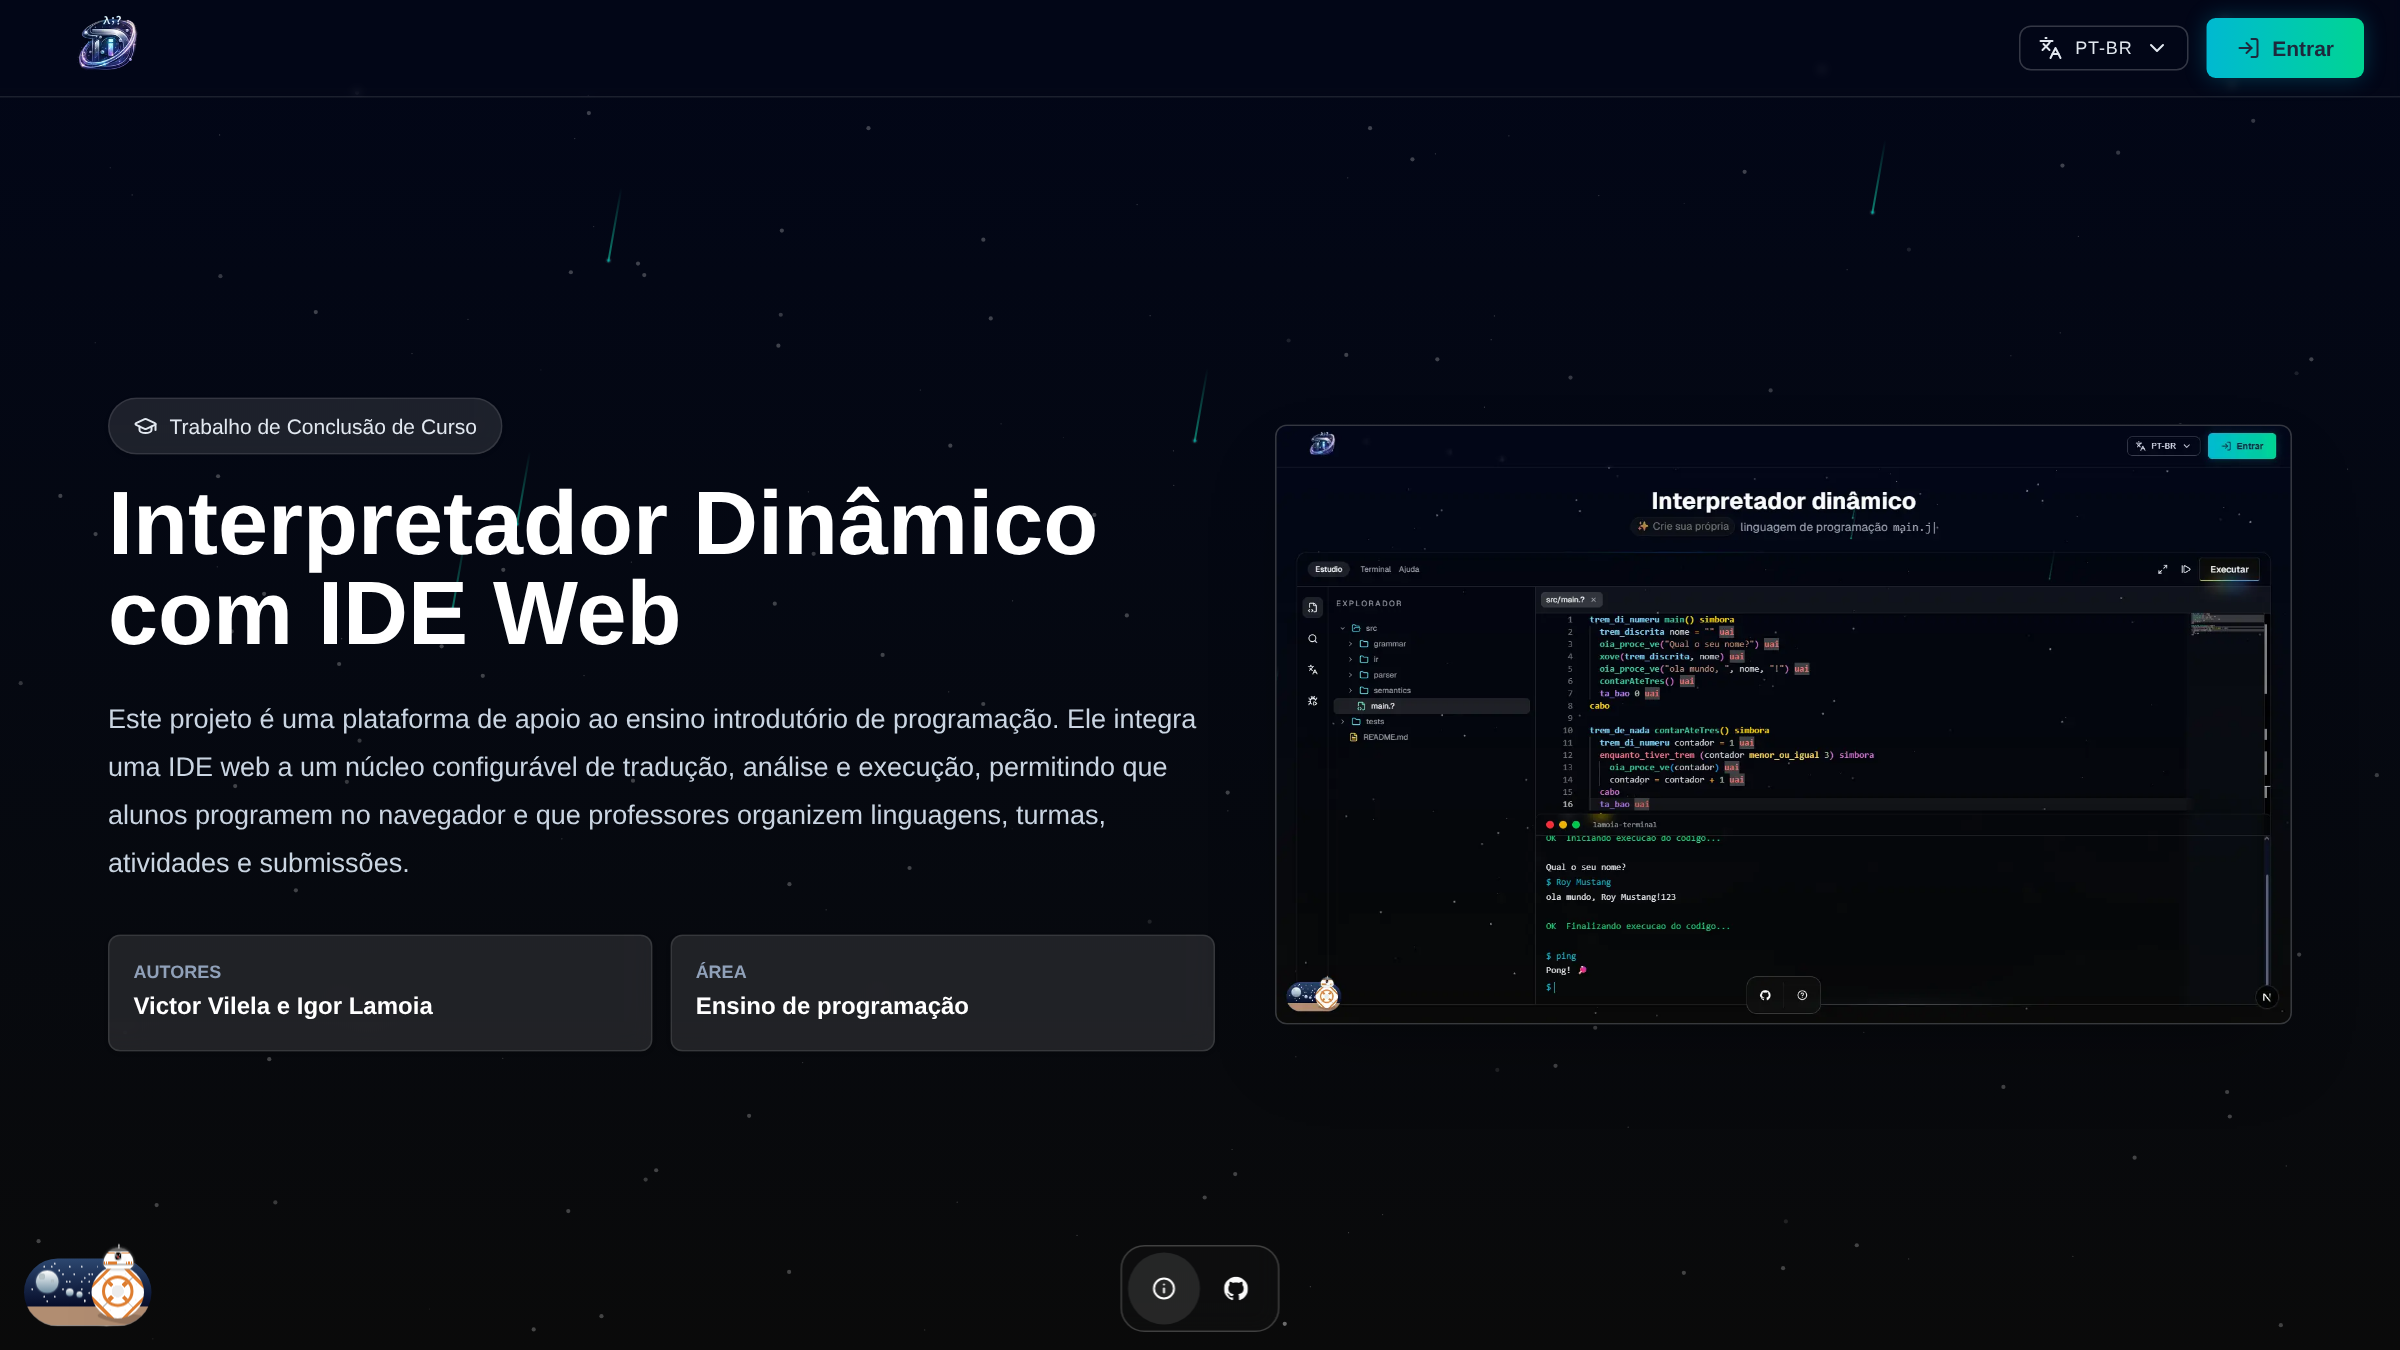
\includegraphics[width=\textwidth,height=0.36\textheight,keepaspectratio]{Sobre/pagina_sobre.png}
    \caption{Página Sobre.}
    \label{fig:pagina-sobre}
    \legend{Fonte: elaborado pelo autor.}
\end{figure}

\section{Apresentação das Telas da Plataforma}
\label{sec:telas-plataforma}

Esta seção apresenta as telas da plataforma na ordem dos requisitos funcionais da Tabela~\ref{tab:requisitos-funcionais}. Cada subseção reúne as telas de um conjunto de requisitos, indicado no título: acesso à plataforma e perfil (RF01 e RF02), personalização da linguagem (RF03 a RF06), linguagens salvas e catálogo da comunidade (RF07 e RF08), depuração e mensagens de erro (RF13 e RF14), turmas (RF15) e exercícios, listas e submissões (RF16 a RF20). As telas ligadas aos demais requisitos já apareceram nas seções anteriores: a IDE, com o editor, o explorador de arquivos, o terminal e os \textit{tokens} (RF09 a RF12), nas Figuras~\ref{fig:ide-execucao} e~\ref{fig:ide-analise-lexica}; a resolução de exercício com linguagem obrigatória e o resultado dos casos de teste (RF17 e RF19), na Figura~\ref{fig:aluno-resultado}; e a correção pelo professor (RF20), nas Figuras~\ref{fig:correcao-avaliacao} e~\ref{fig:correcao-ide}. Parte das capturas desta seção foi feita em etapas anteriores do desenvolvimento e registra os fluxos, sem reproduzir toda a aparência da versão atual.

\subsection{Acesso à plataforma e identidade visual (RF01)}

A página inicial apresenta a identidade visual da plataforma e é a porta de entrada para a autenticação, a navegação e a divulgação dos recursos disponíveis. A composição segue o sistema de temas claro e escuro descrito na Seção~\ref{sec:acessibilidade-responsividade}, com troca controlada pelo \texttt{ThemeContext}, e usa componentes da biblioteca \textit{shadcn/ui}, o que mantém a tipografia e os controles iguais entre as telas. A Figura~\ref{fig:home-light} mostra a página no tema claro.

\begin{figure}[H]
    \centering
    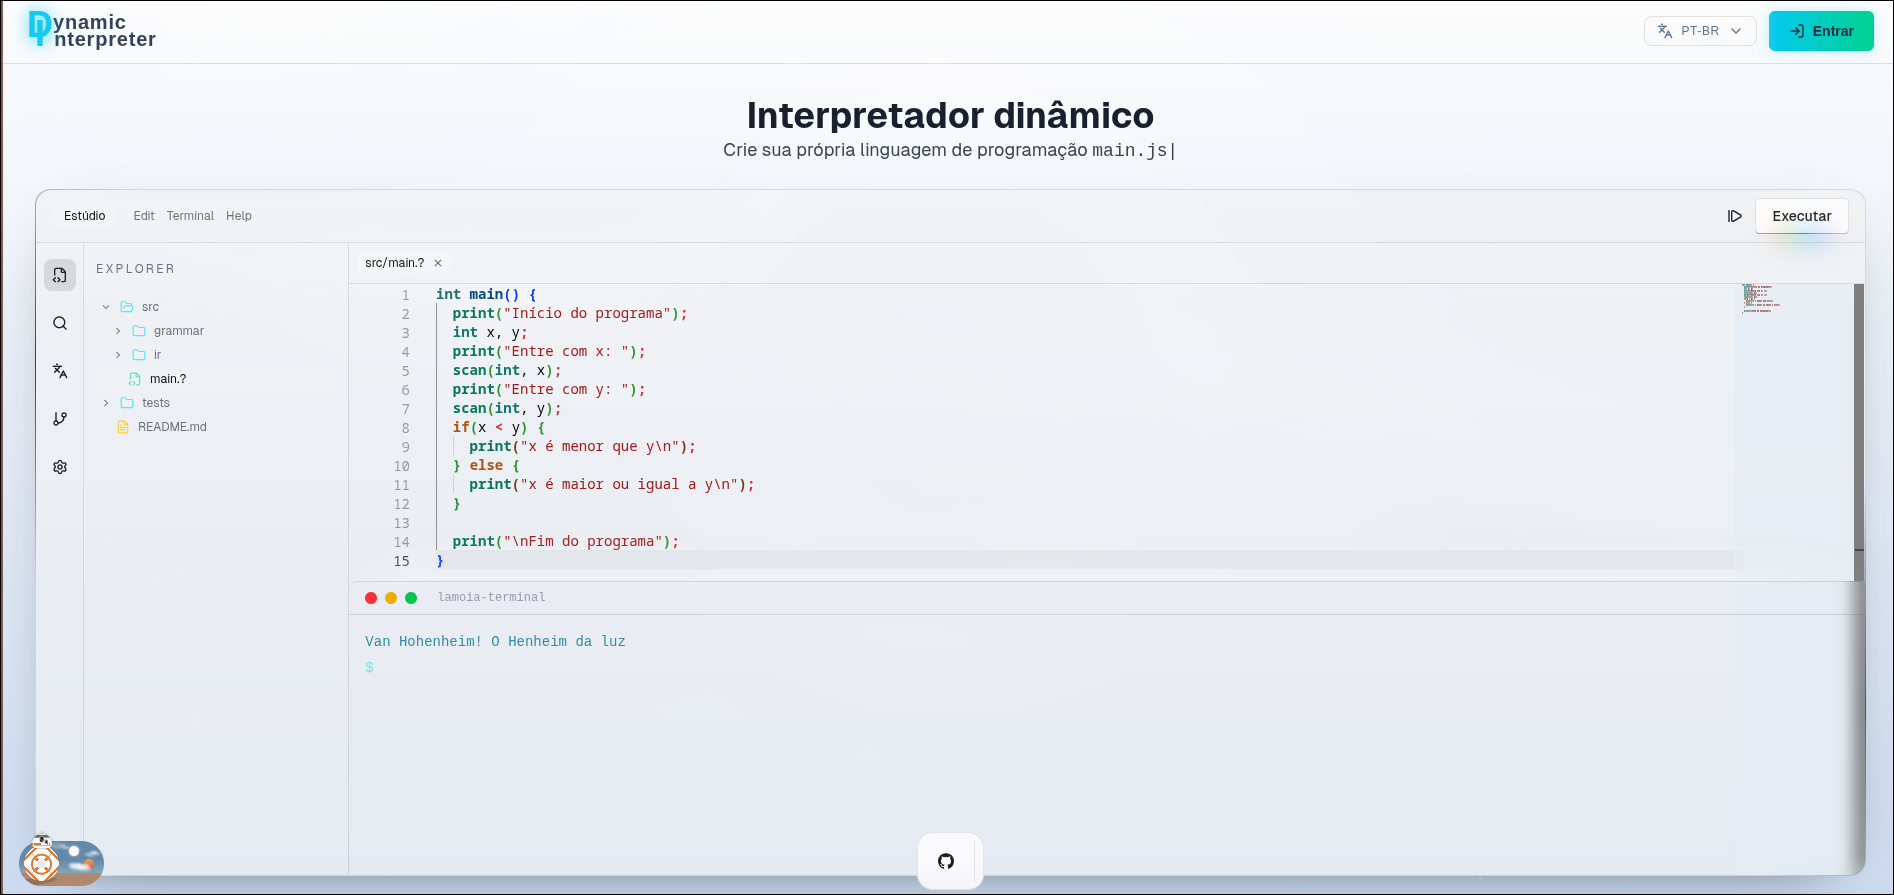
\includegraphics[width=\textwidth,height=0.34\textheight,keepaspectratio]{home_page_light.png}
    \caption{Página inicial da plataforma no tema claro.}
    \label{fig:home-light}
    \legend{Fonte: elaborado pelo autor.}
\end{figure}

A Figura~\ref{fig:home-dark} mostra a mesma página no tema escuro.

\begin{figure}[H]
    \centering
    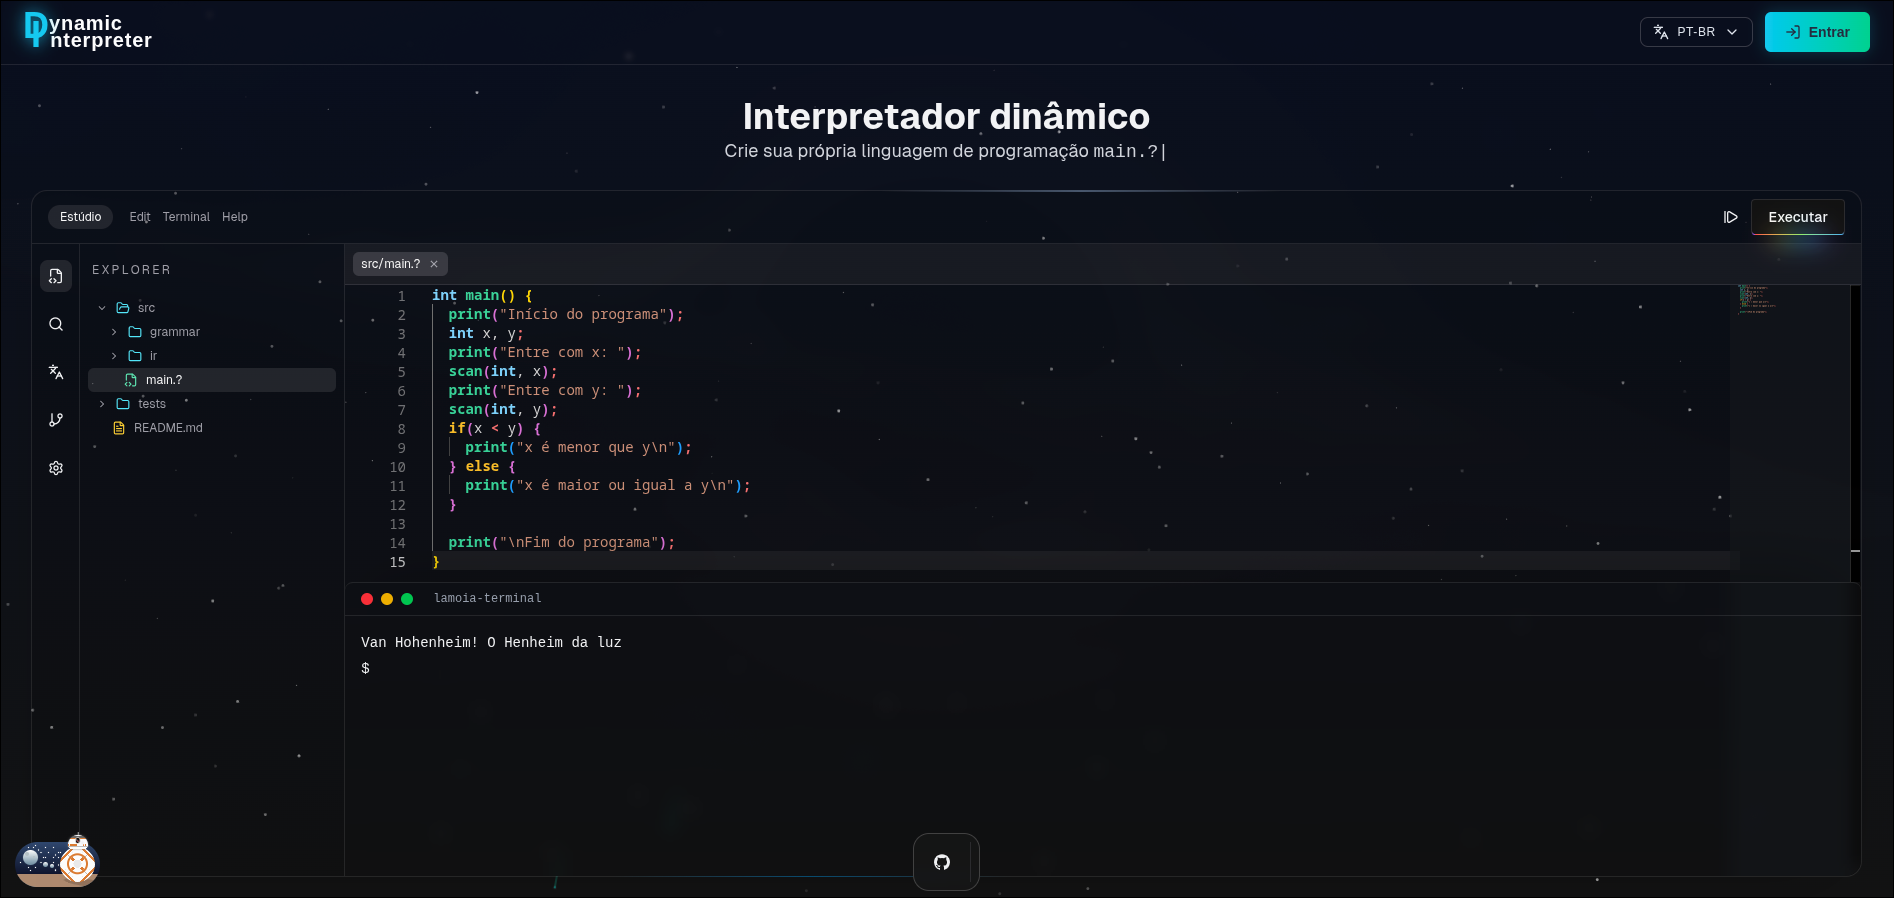
\includegraphics[width=\textwidth,height=0.34\textheight,keepaspectratio]{home_page_dark.png}
    \caption{Página inicial da plataforma no tema escuro.}
    \label{fig:home-dark}
    \legend{Fonte: elaborado pelo autor.}
\end{figure}

\subsection{Perfil do usuário (RF02)}

Depois da autenticação, o nome e o papel do usuário ficam no canto superior direito de todas as páginas. Ao abri-los, o menu dá acesso ao painel e à saída da conta (Figura~\ref{fig:menu-perfil}). A interface mostra os dados do perfil, mas não tem uma tela para editá-los: a alteração de nome, foto e biografia existe no serviço de dados, pela rota \texttt{PATCH /users/\{id\}}, e ainda não foi levada para a IDE. O RF02 está, portanto, atendido na consulta e só parcialmente na edição.

\begin{figure}[H]
    \centering
    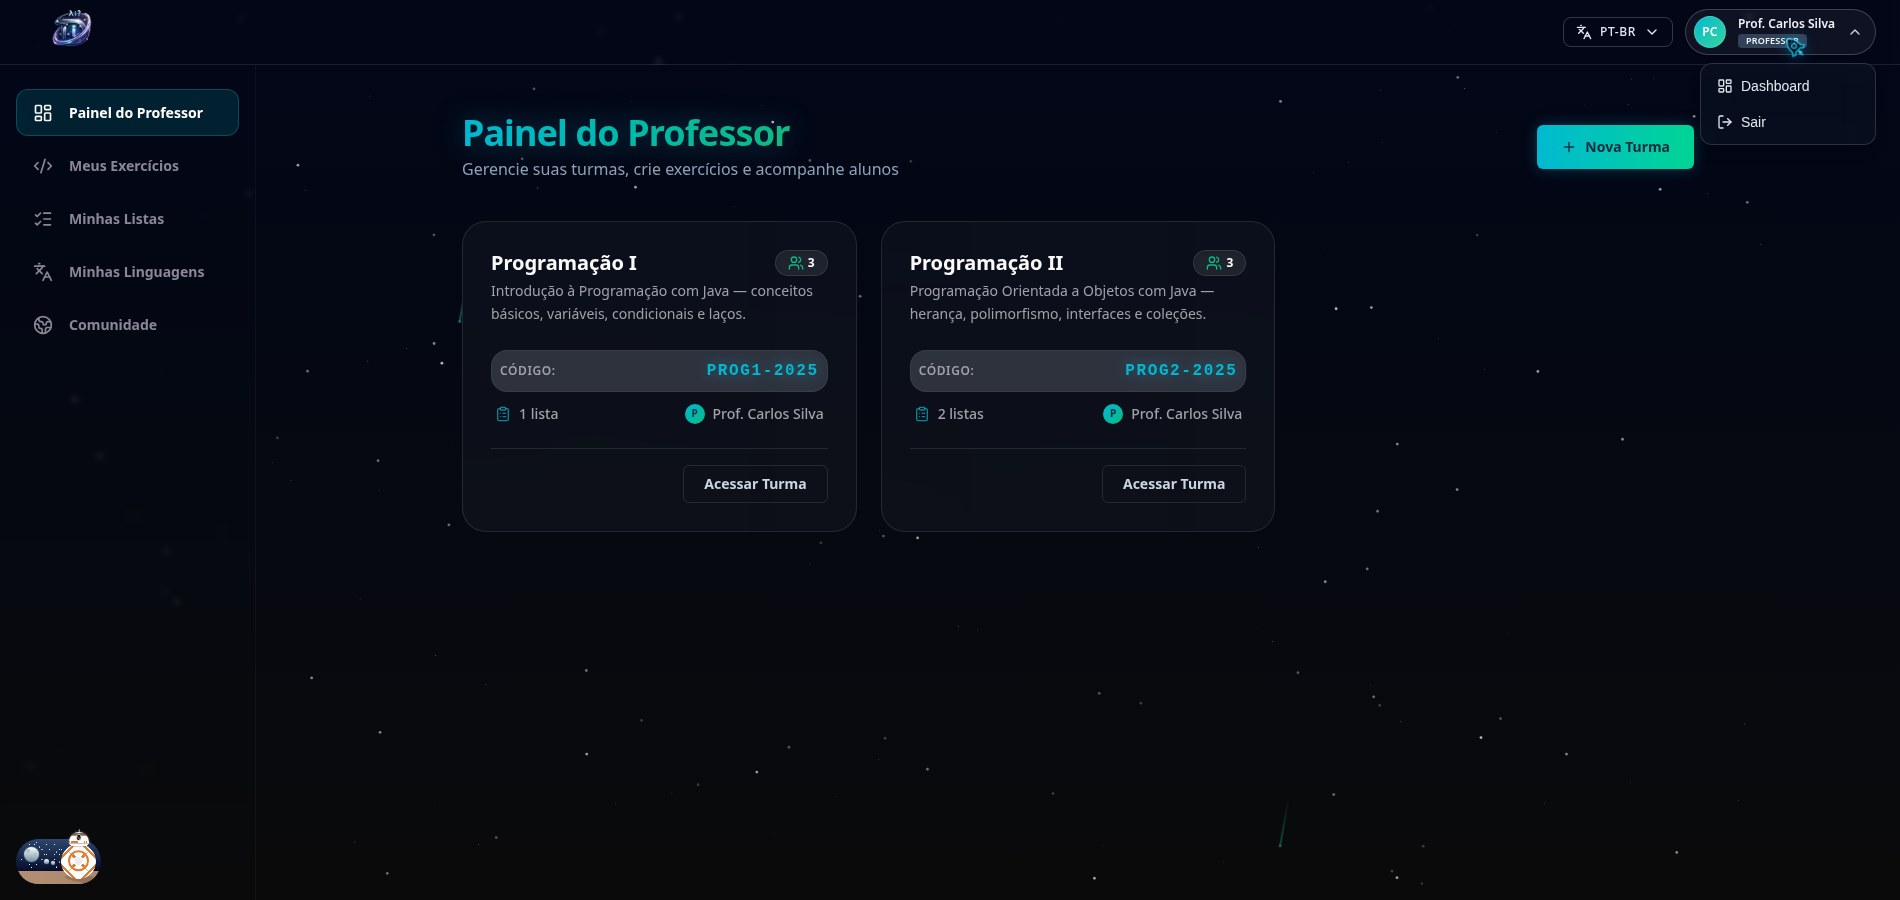
\includegraphics[width=\textwidth,height=0.34\textheight,keepaspectratio]{Perfil/menu_perfil.png}
    \caption{Menu do usuário autenticado, com nome, papel e acesso ao painel.}
    \label{fig:menu-perfil}
    \legend{Fonte: elaborado pelo autor.}
\end{figure}

\subsection{Personalização da linguagem pelo estudante (RF03 a RF06)}

A personalização do vocabulário e das regras estruturais da linguagem foi implementada em um assistente progressivo cuja versão atual contém sete etapas: identidade, entrada/saída, tipagem, estrutura, operadores, fluxo e revisão. Esse \textit{wizard}, descrito na Seção~\ref{sec:customizacao-dinamica}, conduz o usuário por escolhas independentes, validadas isoladamente, com geração de \textit{preview} em tempo real do código resultante. A versão atual aparece nas Figuras~\ref{fig:responsividade-wizard} e~\ref{fig:responsividade-wizard-celular}, da verificação técnica descrita na Seção~\ref{subsec:verificacao-interface}. As capturas a seguir registram a organização anterior, em seis etapas, preservada como histórico da implementação; não representam a sequência atual.

A primeira etapa define o nome da linguagem e a identidade da customização (Figura~\ref{fig:etapa1}).

\begin{figure}[H]
    \centering
    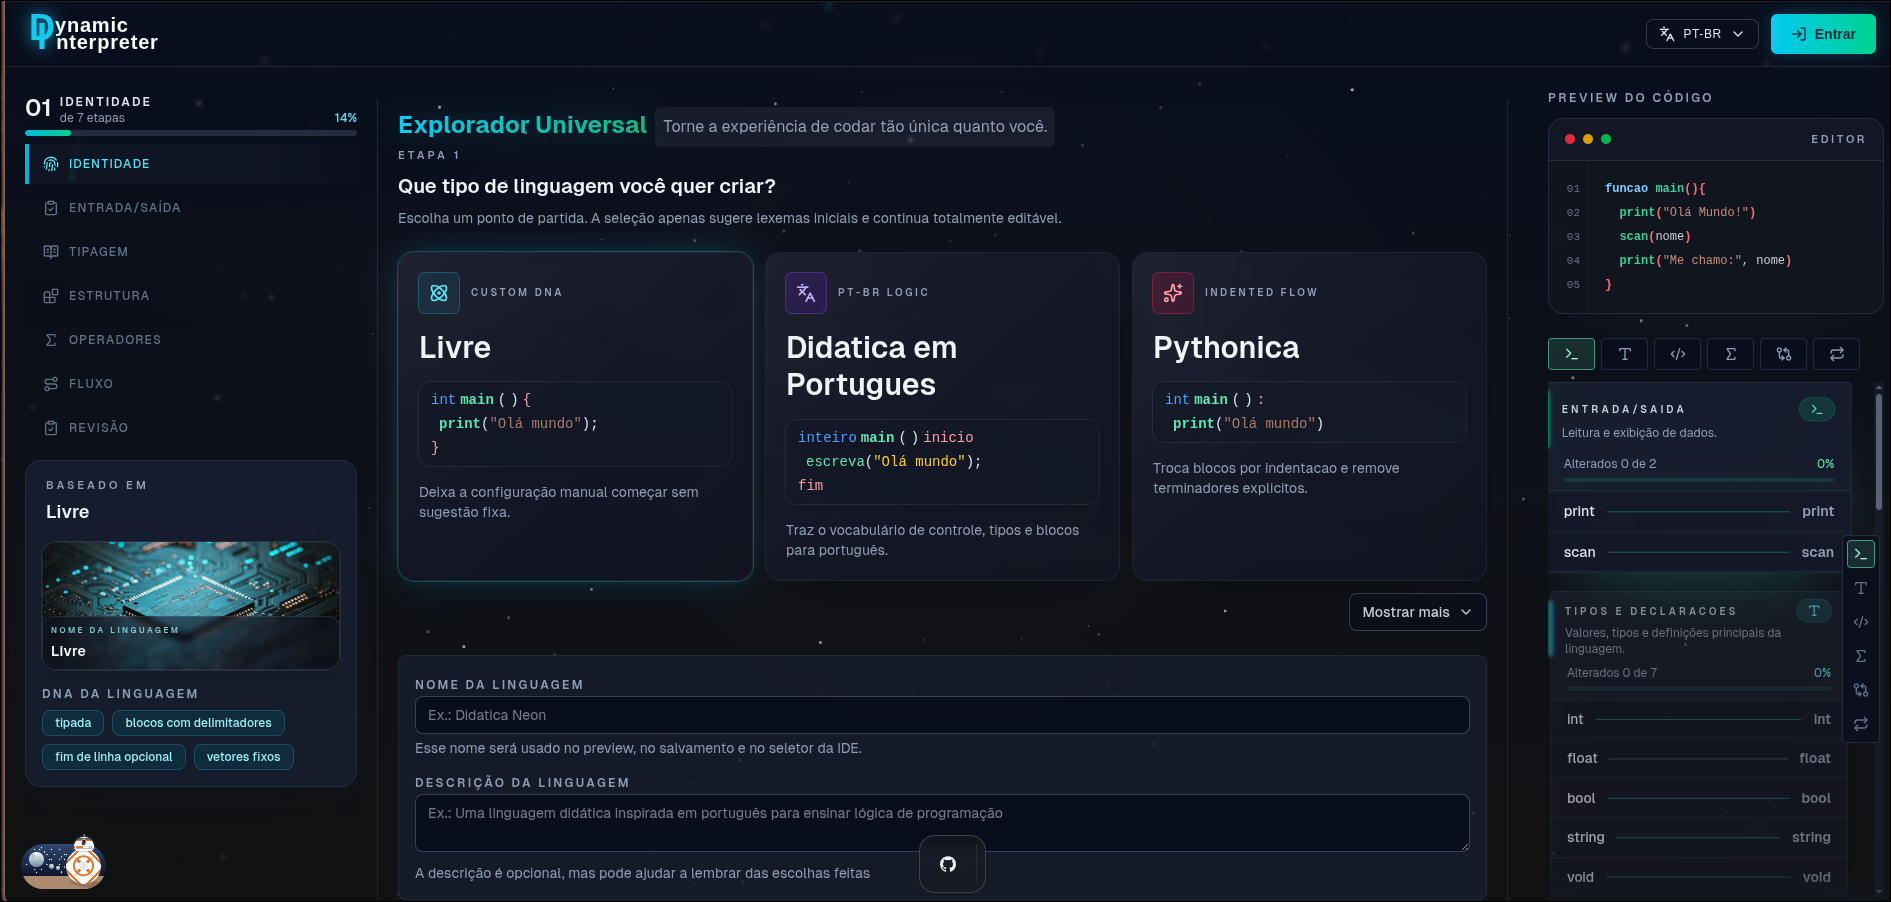
\includegraphics[width=\textwidth,height=0.34\textheight,keepaspectratio]{Etapas/etapa1.png}
    \caption{Etapa 1 do assistente: definição do nome da linguagem e da identidade da customização.}
    \label{fig:etapa1}
    \legend{Fonte: elaborado pelo autor.}
\end{figure}

Na segunda etapa, o usuário configura as palavras-chave dos tipos primitivos (Figura~\ref{fig:etapa2}).

\begin{figure}[H]
    \centering
    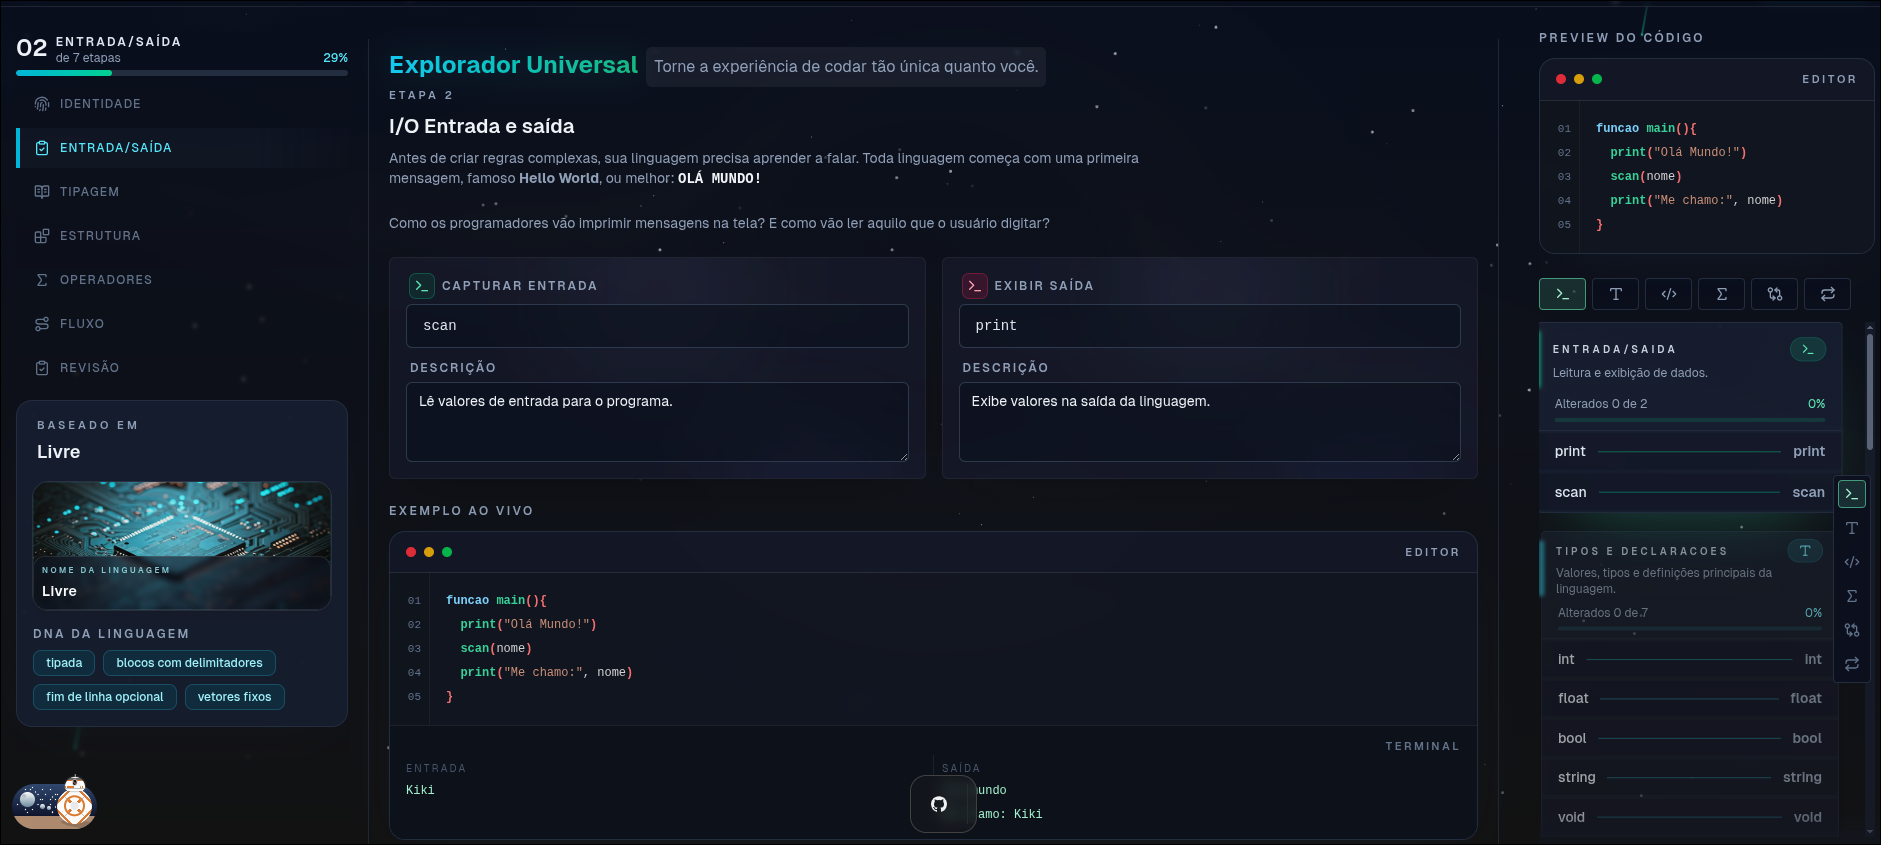
\includegraphics[width=\textwidth,height=0.34\textheight,keepaspectratio]{Etapas/etapa2.png}
    \caption{Etapa 2 do assistente: configuração das palavras-chave de tipos primitivos.}
    \label{fig:etapa2}
    \legend{Fonte: elaborado pelo autor.}
\end{figure}

A terceira etapa permite redefinir as palavras-chave de controle de fluxo, como \texttt{if}, \texttt{else}, \texttt{for}, \texttt{while}, \texttt{break}, \texttt{continue} e \texttt{return}. Ela tem duas partes. A Figura~\ref{fig:etapa3-1} mostra a configuração das palavras-chave básicas.

\begin{figure}[H]
    \centering
    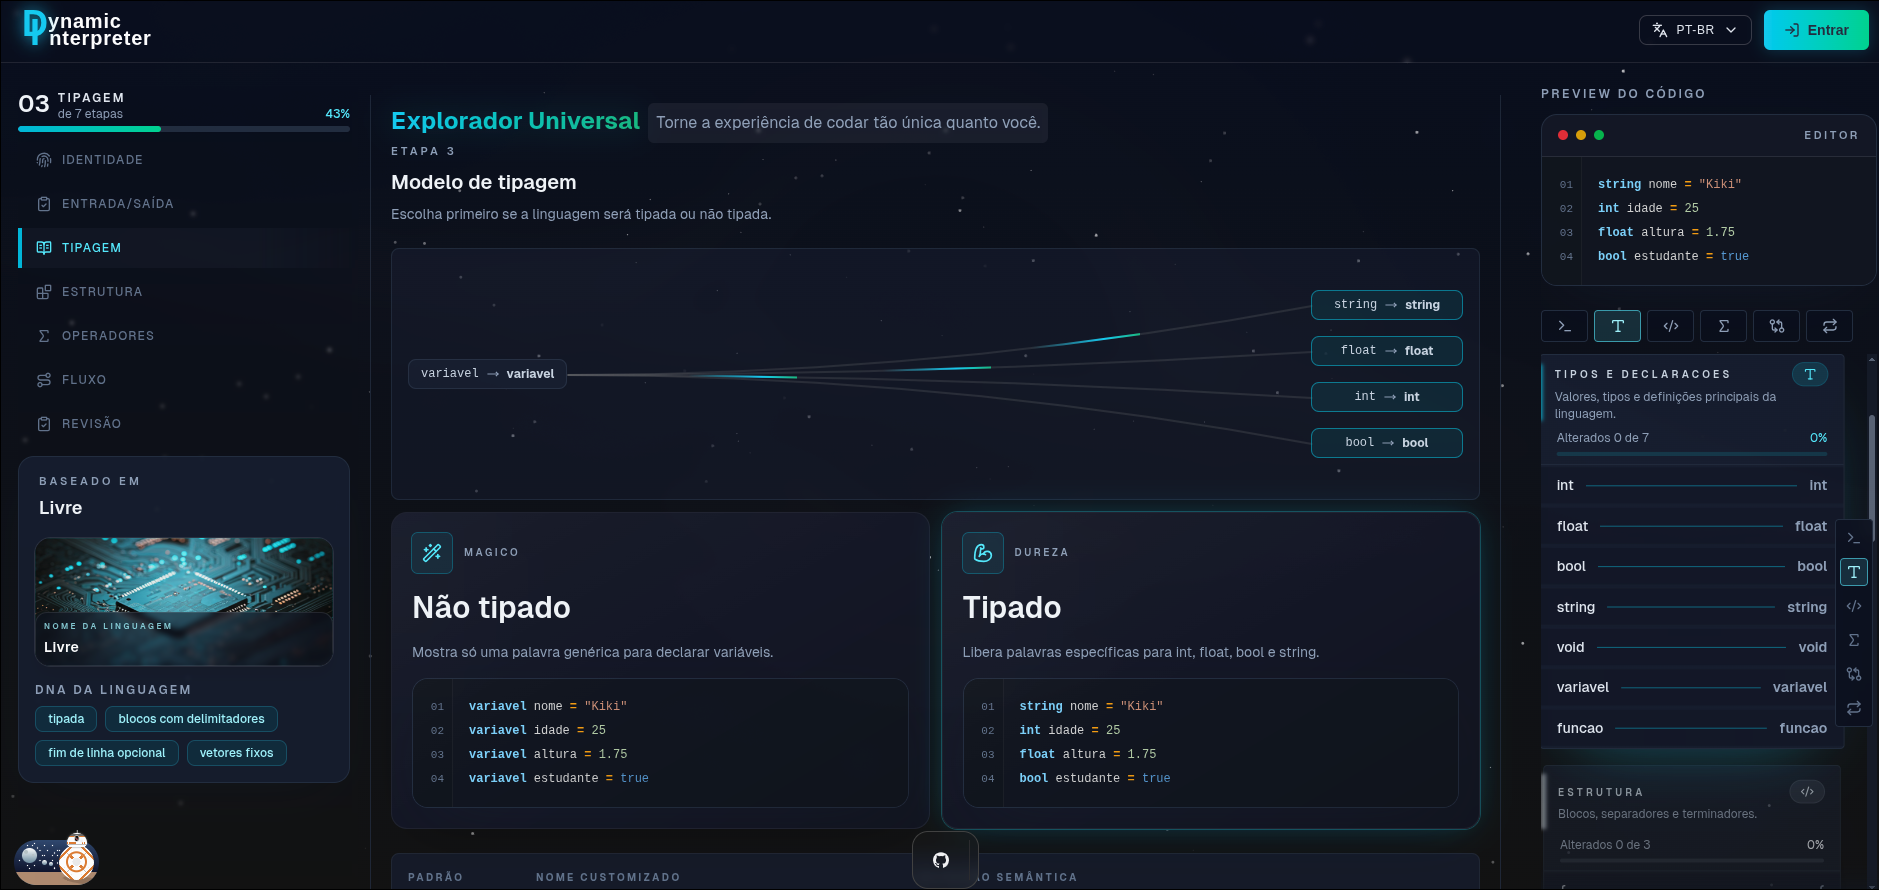
\includegraphics[width=\textwidth,height=0.34\textheight,keepaspectratio]{Etapas/etapa3_1.png}
    \caption{Etapa 3 do assistente, primeira parte: palavras-chave básicas de controle de fluxo.}
    \label{fig:etapa3-1}
    \legend{Fonte: elaborado pelo autor.}
\end{figure}

A Figura~\ref{fig:etapa3-2} mostra a segunda parte, com a configuração estendida de construtores como \texttt{switch} e \texttt{case}.

\begin{figure}[H]
    \centering
    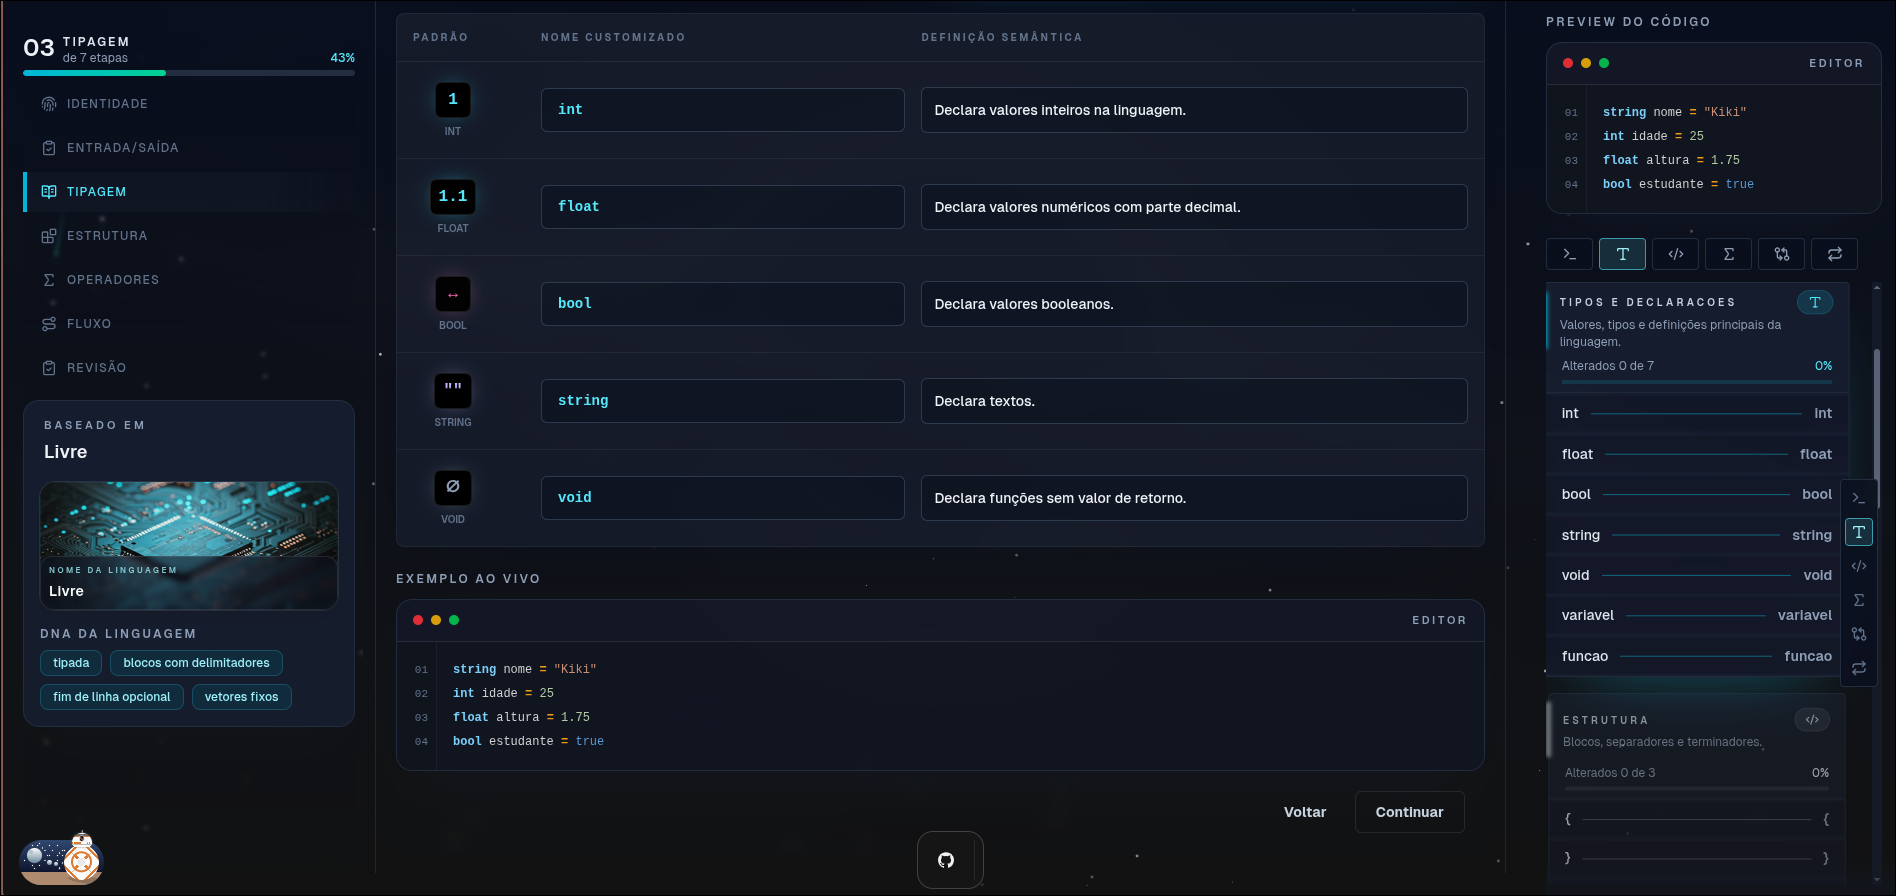
\includegraphics[width=\textwidth,height=0.34\textheight,keepaspectratio]{Etapas/etapa3_2.png}
    \caption{Etapa 3 do assistente, segunda parte: construtores estendidos de controle de fluxo.}
    \label{fig:etapa3-2}
    \legend{Fonte: elaborado pelo autor.}
\end{figure}

A quarta etapa permite substituir operadores lógicos e relacionais por palavras de uso natural, como uma alternativa de escrita a ser investigada, motivada pela discussão de escolhas sintáticas de \citeonline{stefik2013}. Primeiro, o usuário define os operadores lógicos, como \texttt{e}, \texttt{ou} e \texttt{não} (Figura~\ref{fig:etapa4-1}).

\begin{figure}[H]
    \centering
    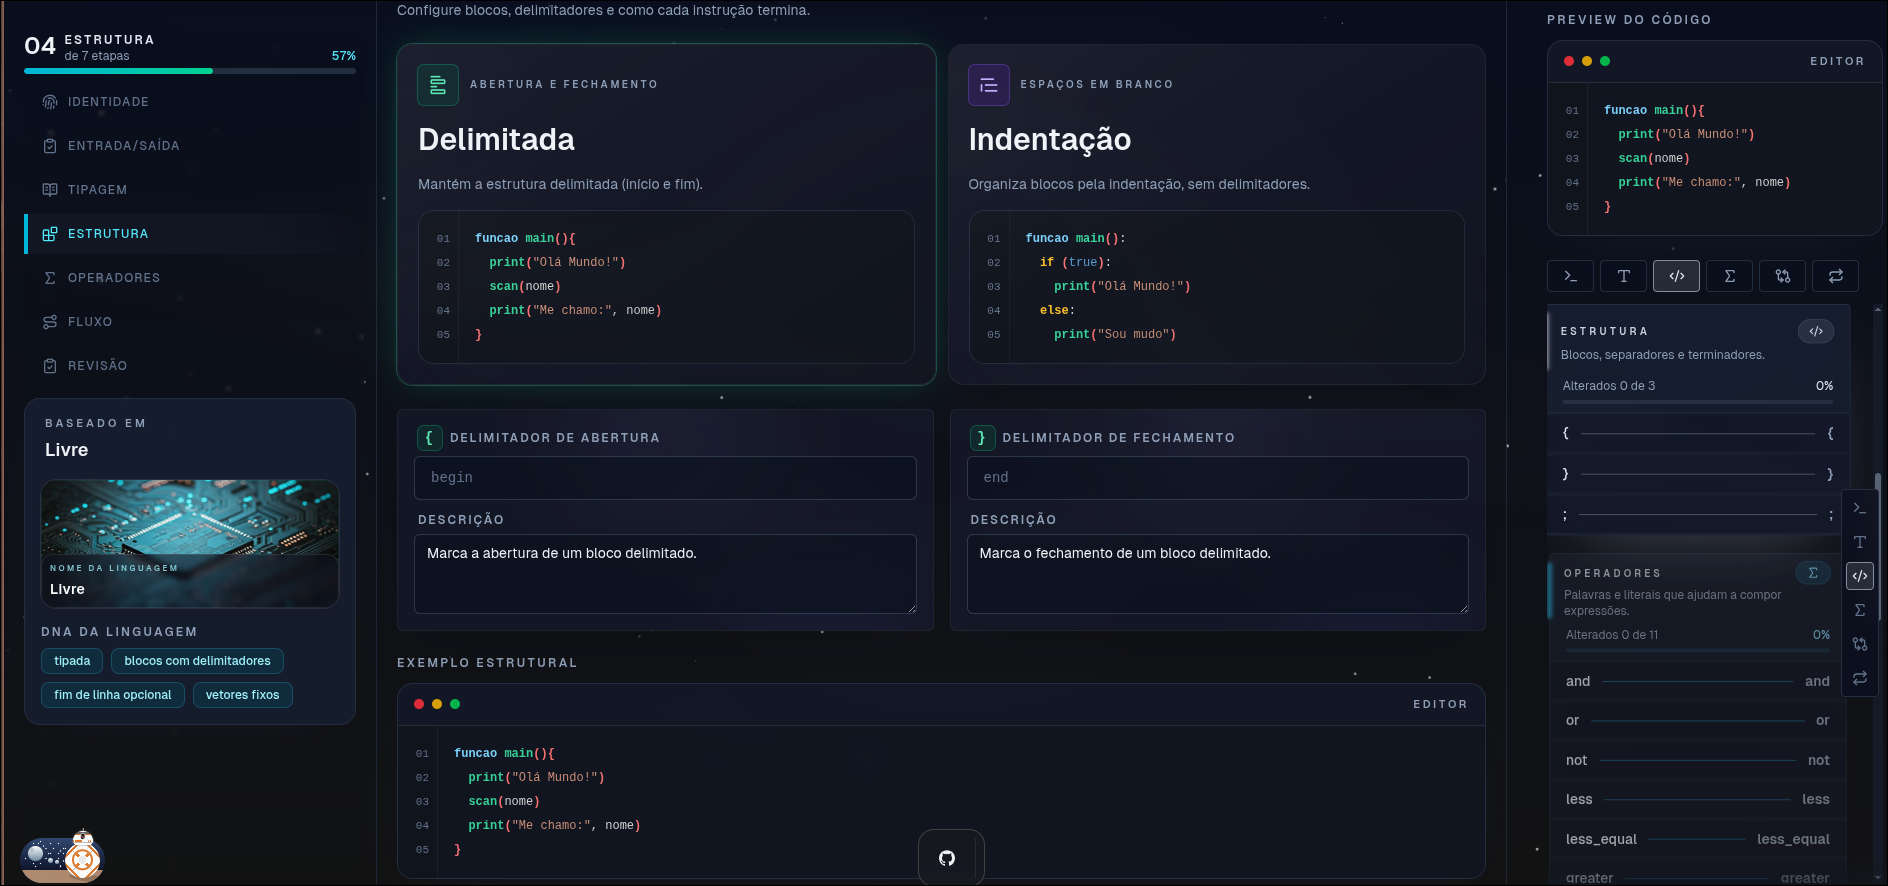
\includegraphics[width=\textwidth,height=0.34\textheight,keepaspectratio]{Etapas/etapa4_1.png}
    \caption{Etapa 4 do assistente, primeira parte: operadores lógicos em forma de palavra.}
    \label{fig:etapa4-1}
    \legend{Fonte: elaborado pelo autor.}
\end{figure}

Em seguida, redefine os operadores relacionais pelo mesmo princípio de palavras significativas (Figura~\ref{fig:etapa4-2}).

\begin{figure}[H]
    \centering
    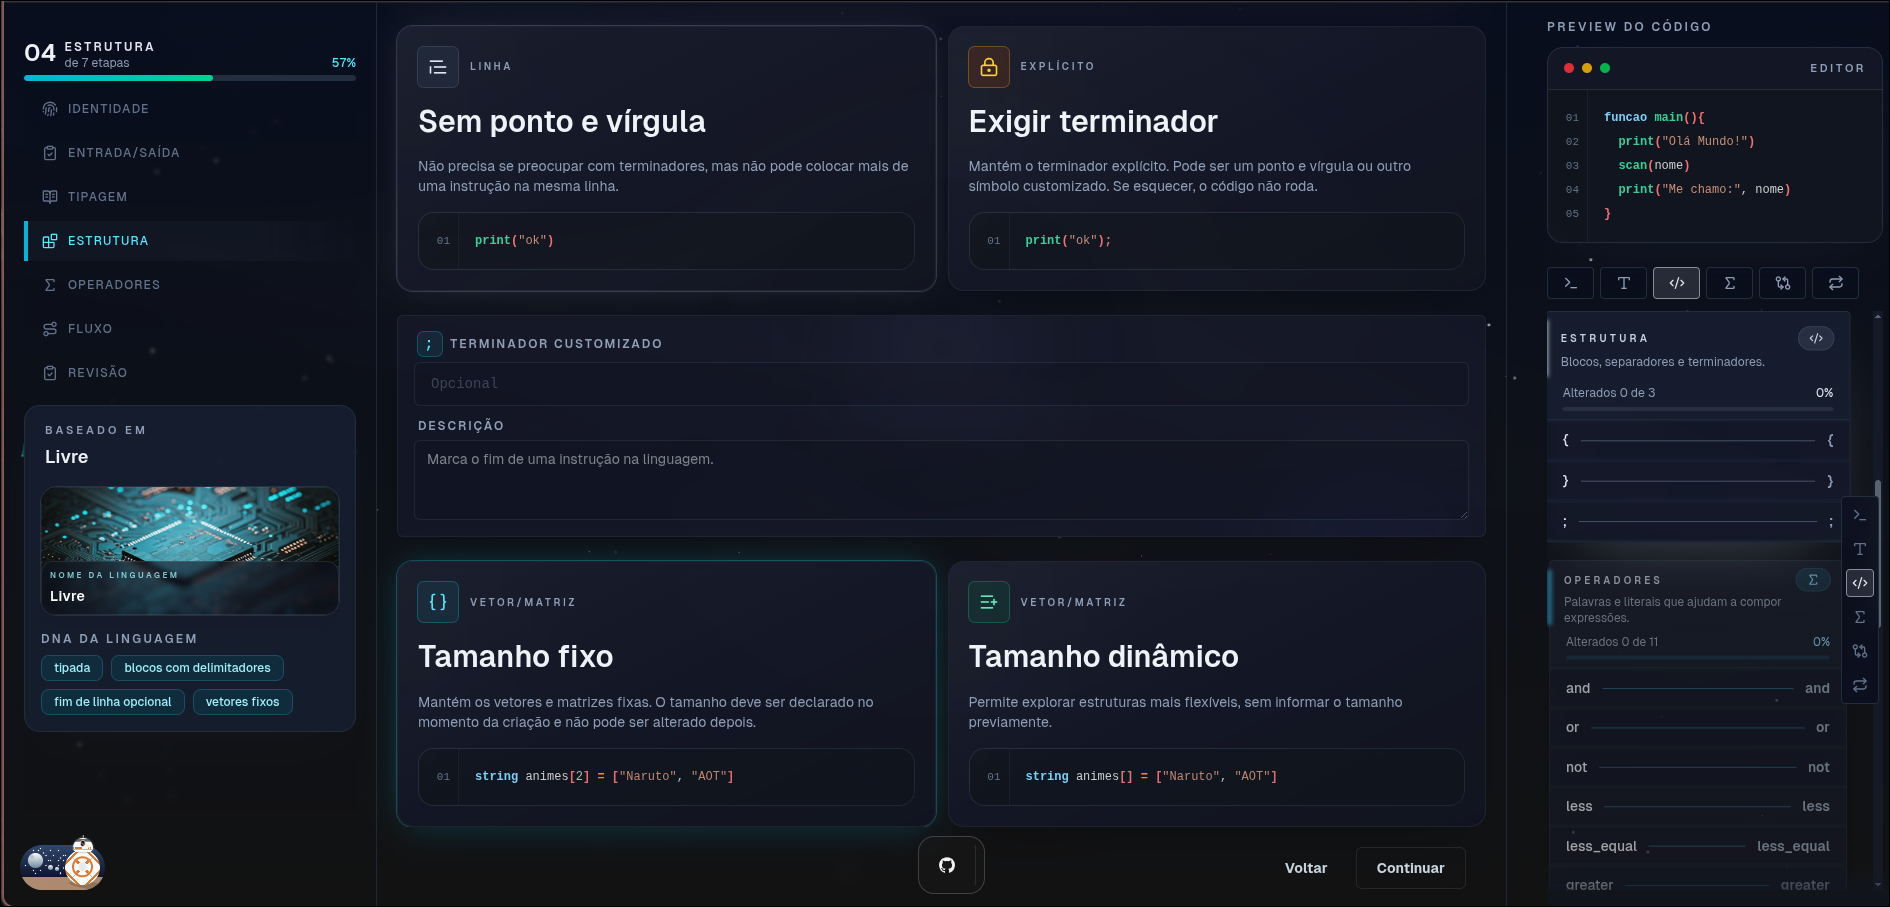
\includegraphics[width=\textwidth,height=0.34\textheight,keepaspectratio]{Etapas/etapa4_2.png}
    \caption{Etapa 4 do assistente, segunda parte: operadores relacionais em forma de palavra.}
    \label{fig:etapa4-2}
    \legend{Fonte: elaborado pelo autor.}
\end{figure}

A quinta etapa configura os literais booleanos e permite adotar termos como \texttt{verdadeiro} e \texttt{falso} no lugar de \texttt{true} e \texttt{false} (Figura~\ref{fig:etapa5}).

\begin{figure}[H]
    \centering
    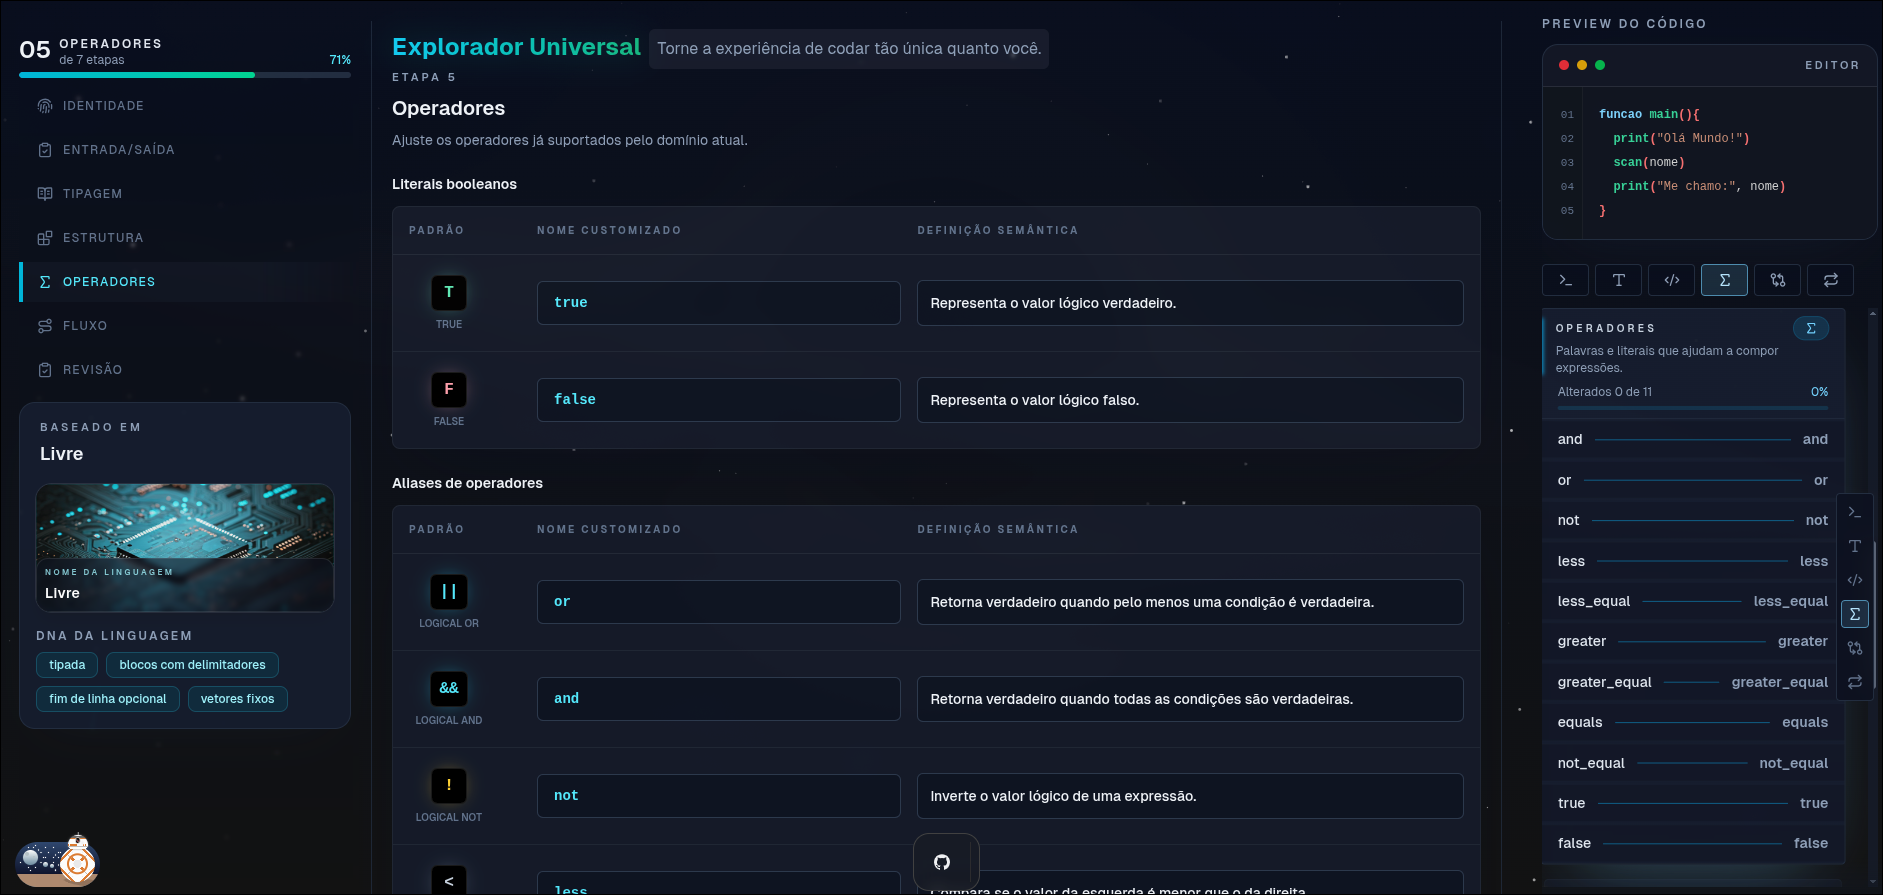
\includegraphics[height=7cm,keepaspectratio]{Etapas/etapa5_1.png}
    \caption{Etapa 5 do assistente: personalização dos literais booleanos.}
    \label{fig:etapa5}
    \legend{Fonte: elaborado pelo autor.}
\end{figure}

A sexta e última etapa dessa versão define os delimitadores de bloco, que podem ser chaves, palavras-chave ou indentação (Figura~\ref{fig:etapa6-1}).

\begin{figure}[H]
    \centering
    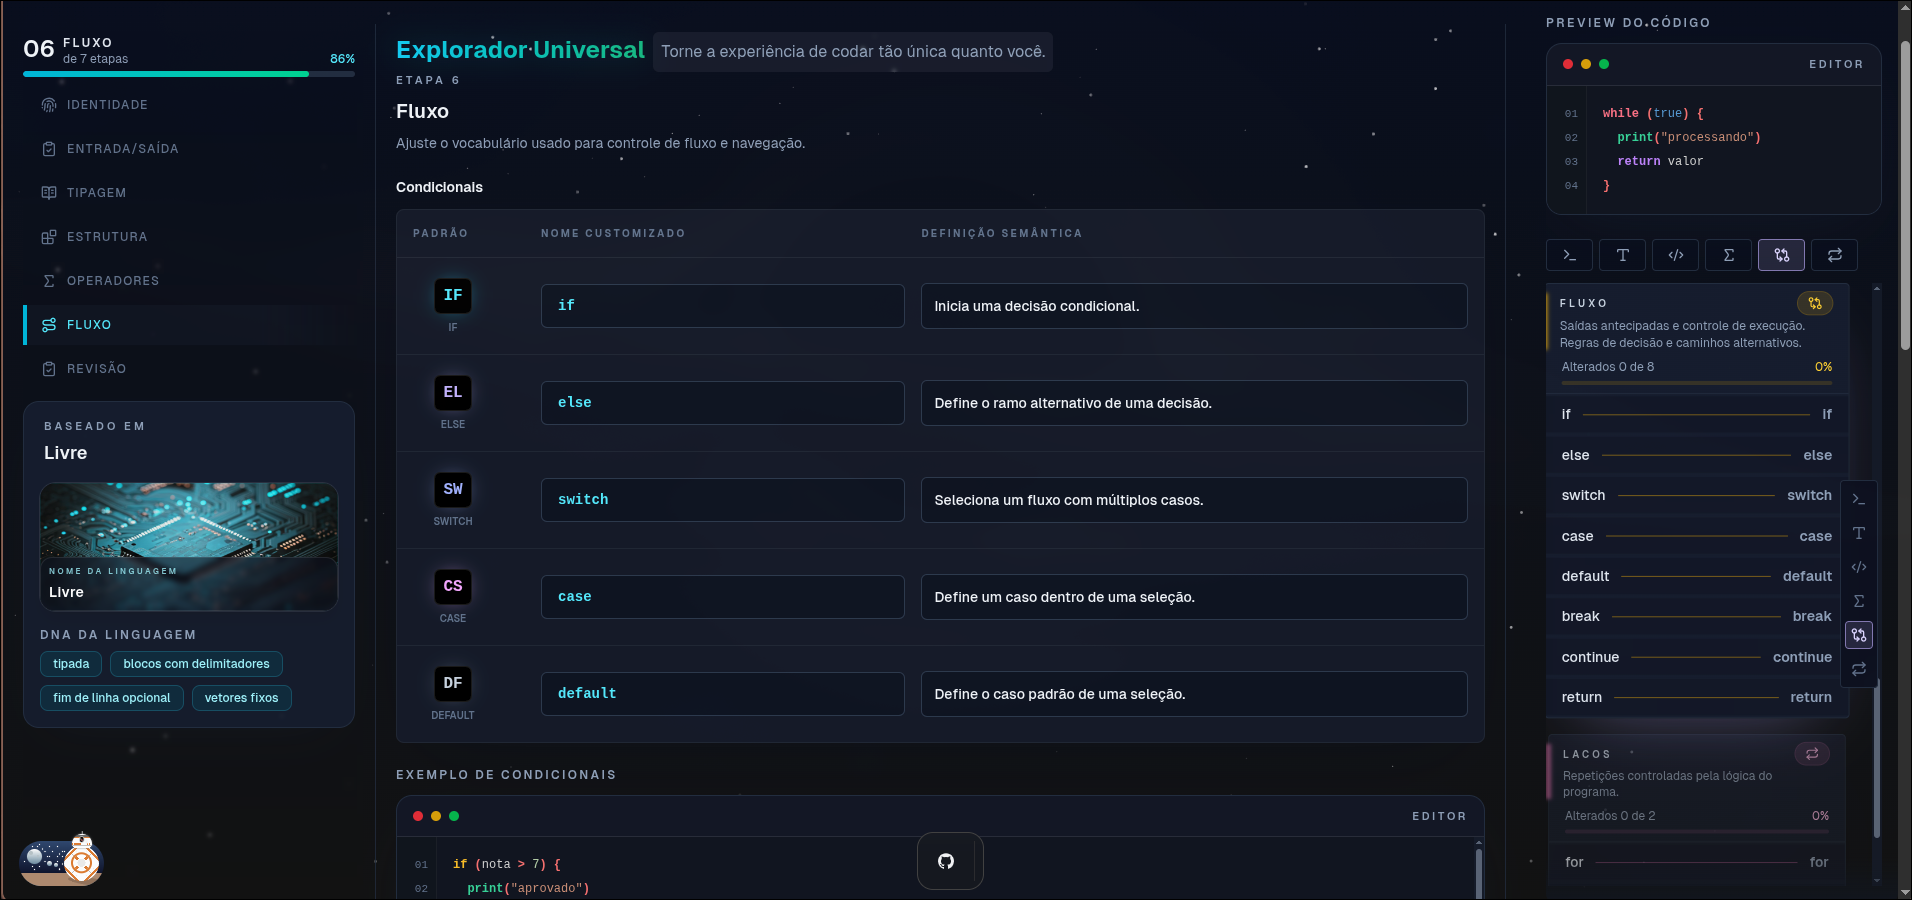
\includegraphics[width=\textwidth,height=0.34\textheight,keepaspectratio]{Etapas/etapa6_1.png}
    \caption{Etapa 6 do assistente: definição dos delimitadores de bloco.}
    \label{fig:etapa6-1}
    \legend{Fonte: elaborado pelo autor.}
\end{figure}

Na mesma etapa, o usuário define o terminador de instrução (Figura~\ref{fig:etapa6-2}).

\begin{figure}[H]
    \centering
    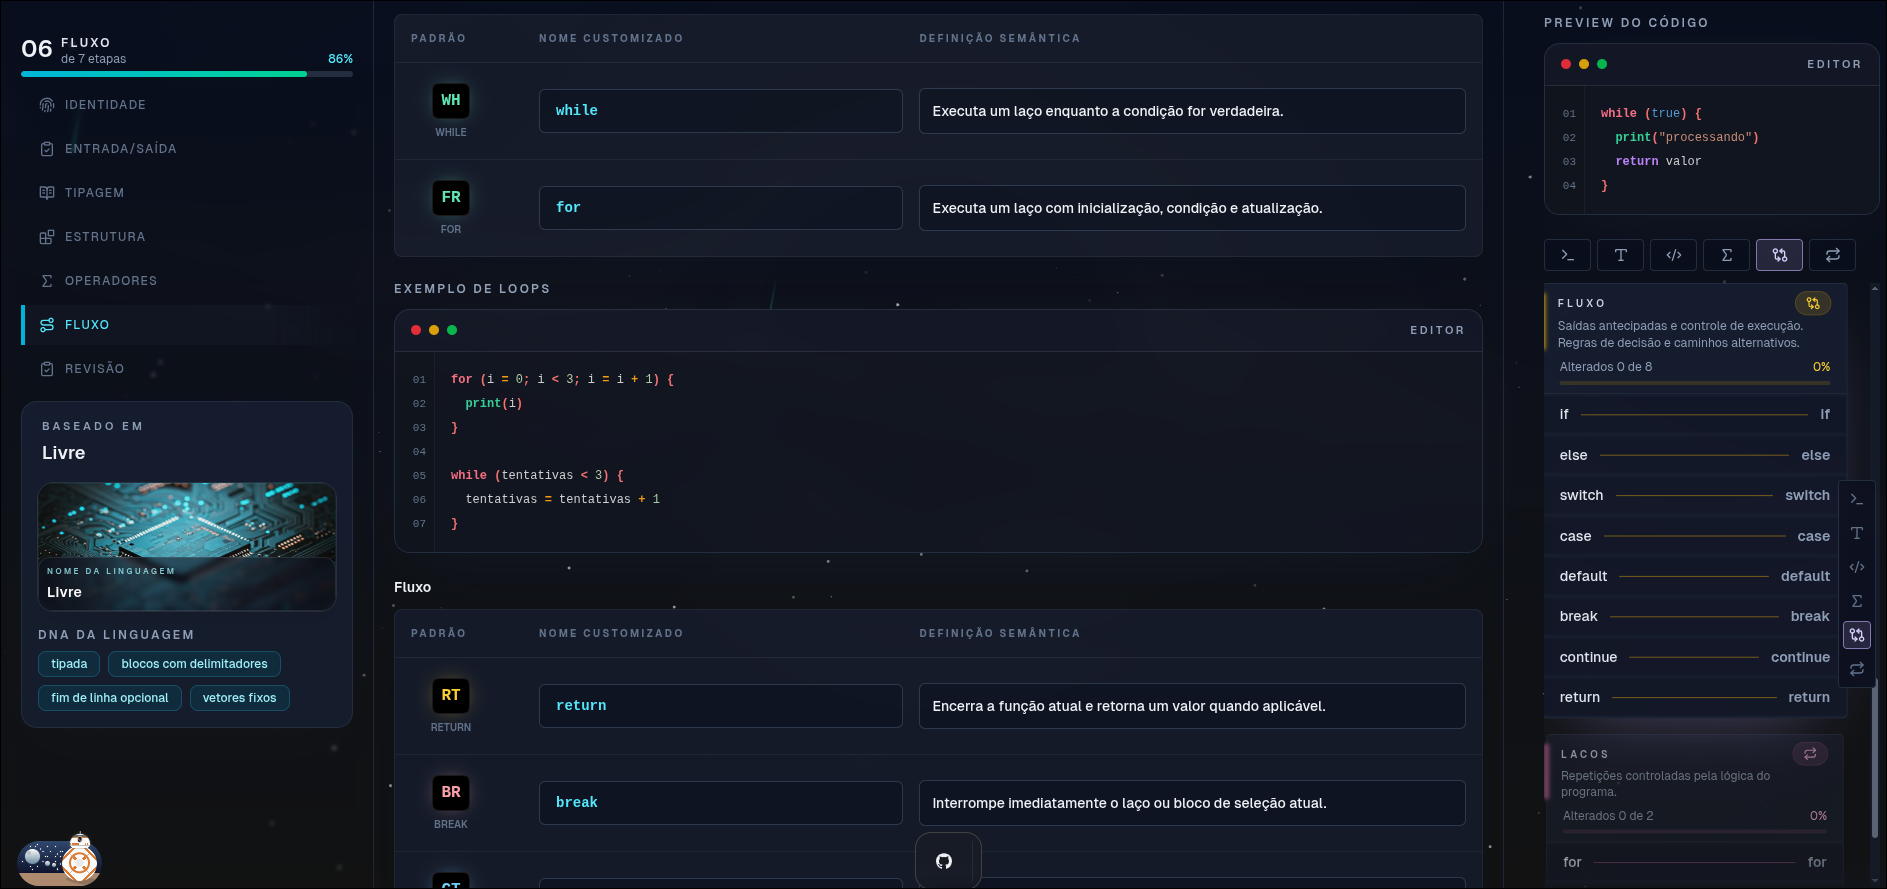
\includegraphics[width=\textwidth,height=0.34\textheight,keepaspectratio]{Etapas/etapa6_2.png}
    \caption{Etapa 6 do assistente: definição do terminador de instrução.}
    \label{fig:etapa6-2}
    \legend{Fonte: elaborado pelo autor.}
\end{figure}

Ao término do assistente, é exibida a pré-visualização consolidada da linguagem personalizada (Figura~\ref{fig:etapa6-3}).

\begin{figure}[H]
    \centering
    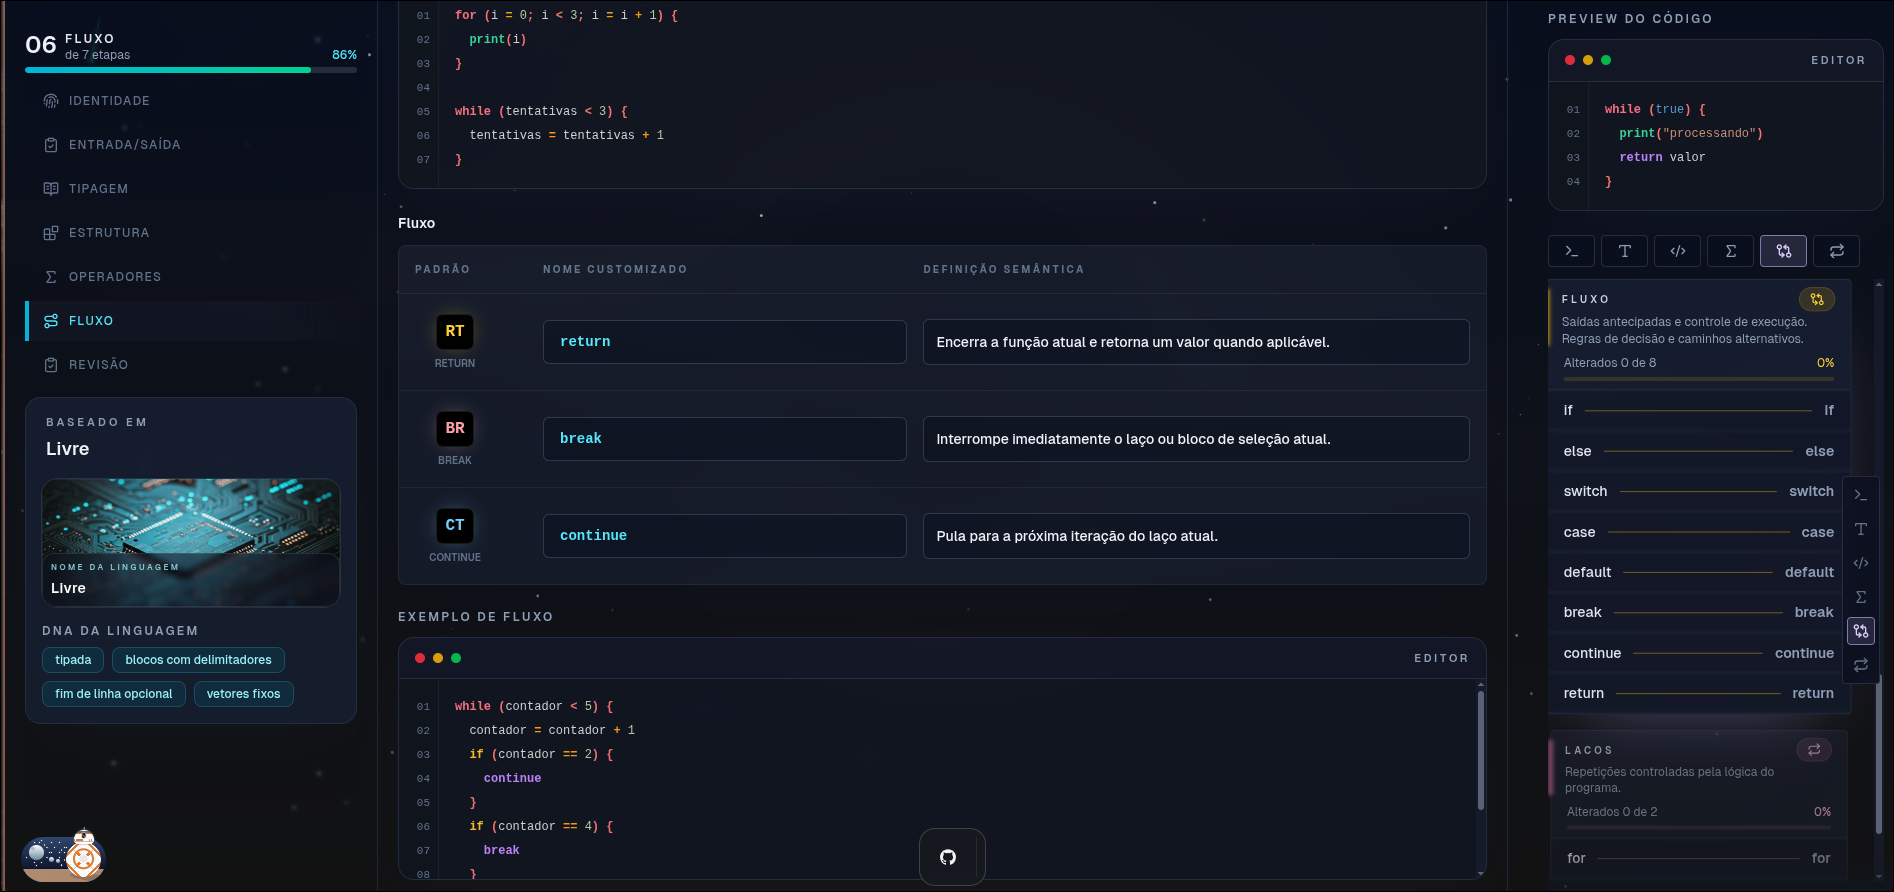
\includegraphics[width=\textwidth,height=0.34\textheight,keepaspectratio]{Etapas/etapa6_3.png}
    \caption{Pré-visualização final da linguagem personalizada, exibida ao término do assistente.}
    \label{fig:etapa6-3}
    \legend{Fonte: elaborado pelo autor.}
\end{figure}

\subsection{Linguagens salvas e catálogo da comunidade (RF07 e RF08)}

As linguagens que o usuário cria ou importa ficam salvas na conta e aparecem na tela ``Minhas Linguagens'', cada uma em um cartão com o nome, a descrição, o resumo das escolhas de tipagem, arranjos, blocos e terminador e as ações de editar, marcar, duplicar e excluir (Figura~\ref{fig:minhas-linguagens}). Na captura, a linguagem ``Minerês (cópia)'' foi importada do catálogo da comunidade.

\begin{figure}[H]
    \centering
    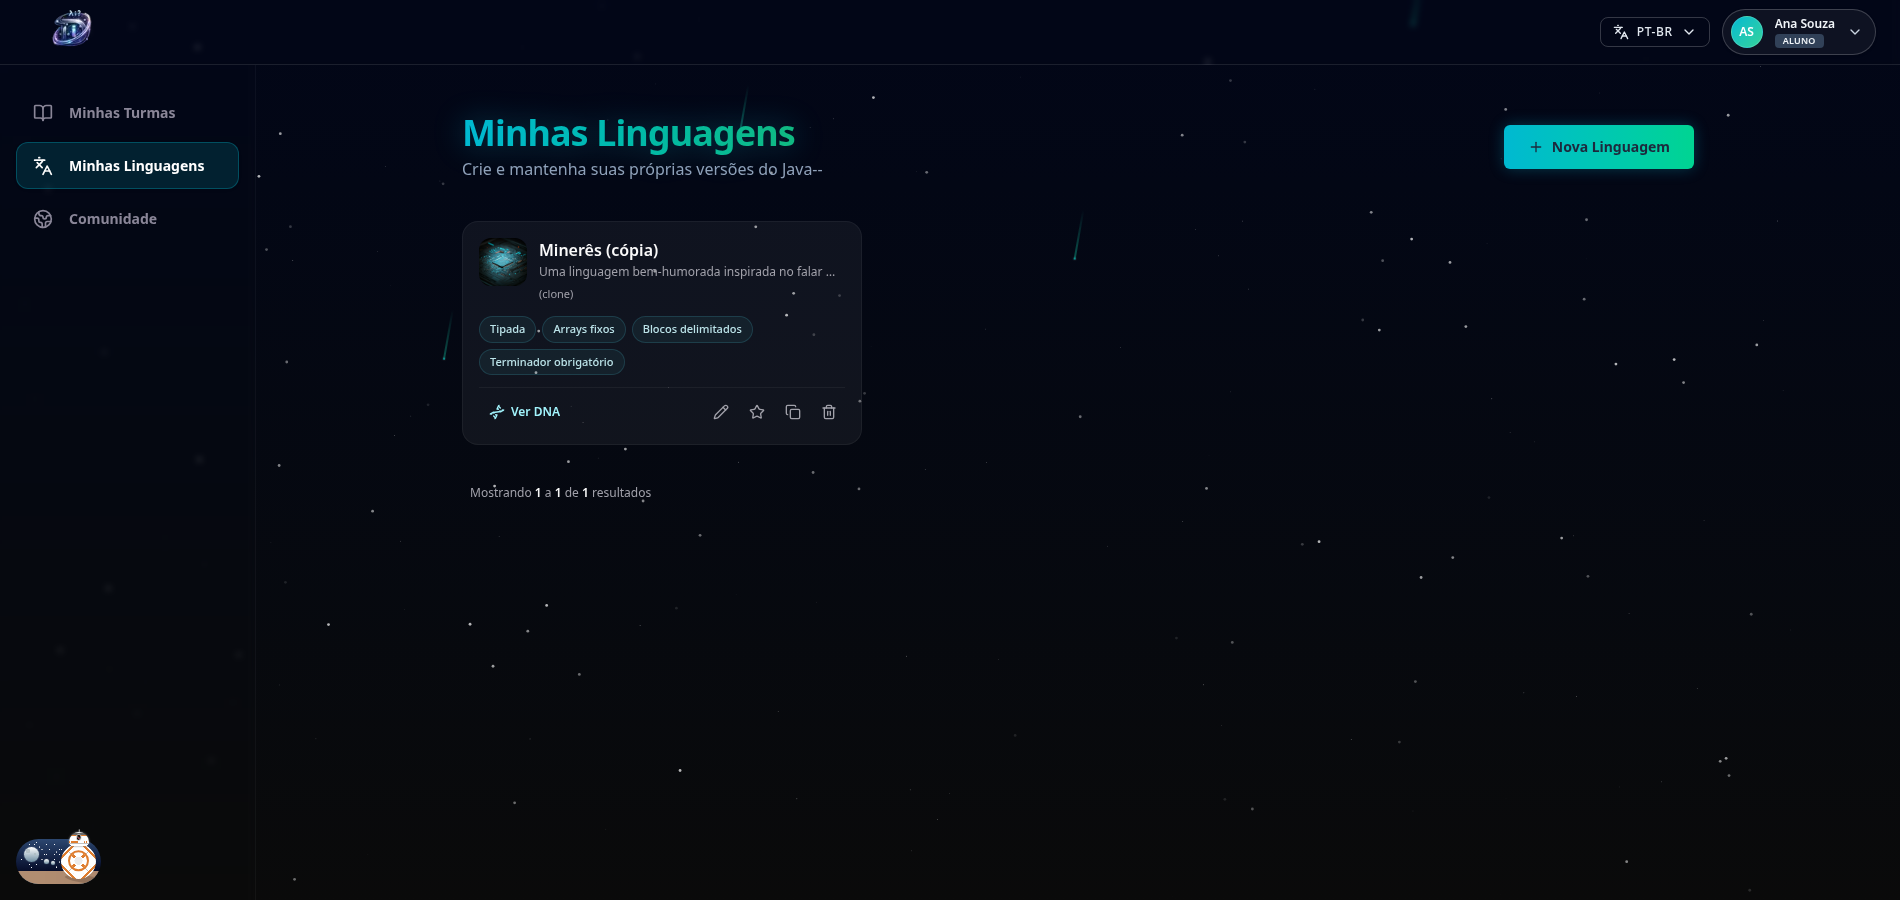
\includegraphics[width=\textwidth,height=0.34\textheight,keepaspectratio]{Linguagens/minhas_linguagens.png}
    \caption{Tela ``Minhas Linguagens'', com uma linguagem salva na conta do aluno.}
    \label{fig:minhas-linguagens}
    \legend{Fonte: elaborado pelo autor.}
\end{figure}

O catálogo da comunidade reúne as linguagens publicadas por outros usuários e as linguagens oficiais da plataforma. Ele permite buscar por nome ou descrição, filtrar pelo modelo de tipagem, pelos blocos, pelos arranjos e pelo terminador, ver o resumo de cada linguagem e importá-la. A importação cria uma cópia privada e editável no acervo de quem importou (Figura~\ref{fig:comunidade}).

\begin{figure}[H]
    \centering
    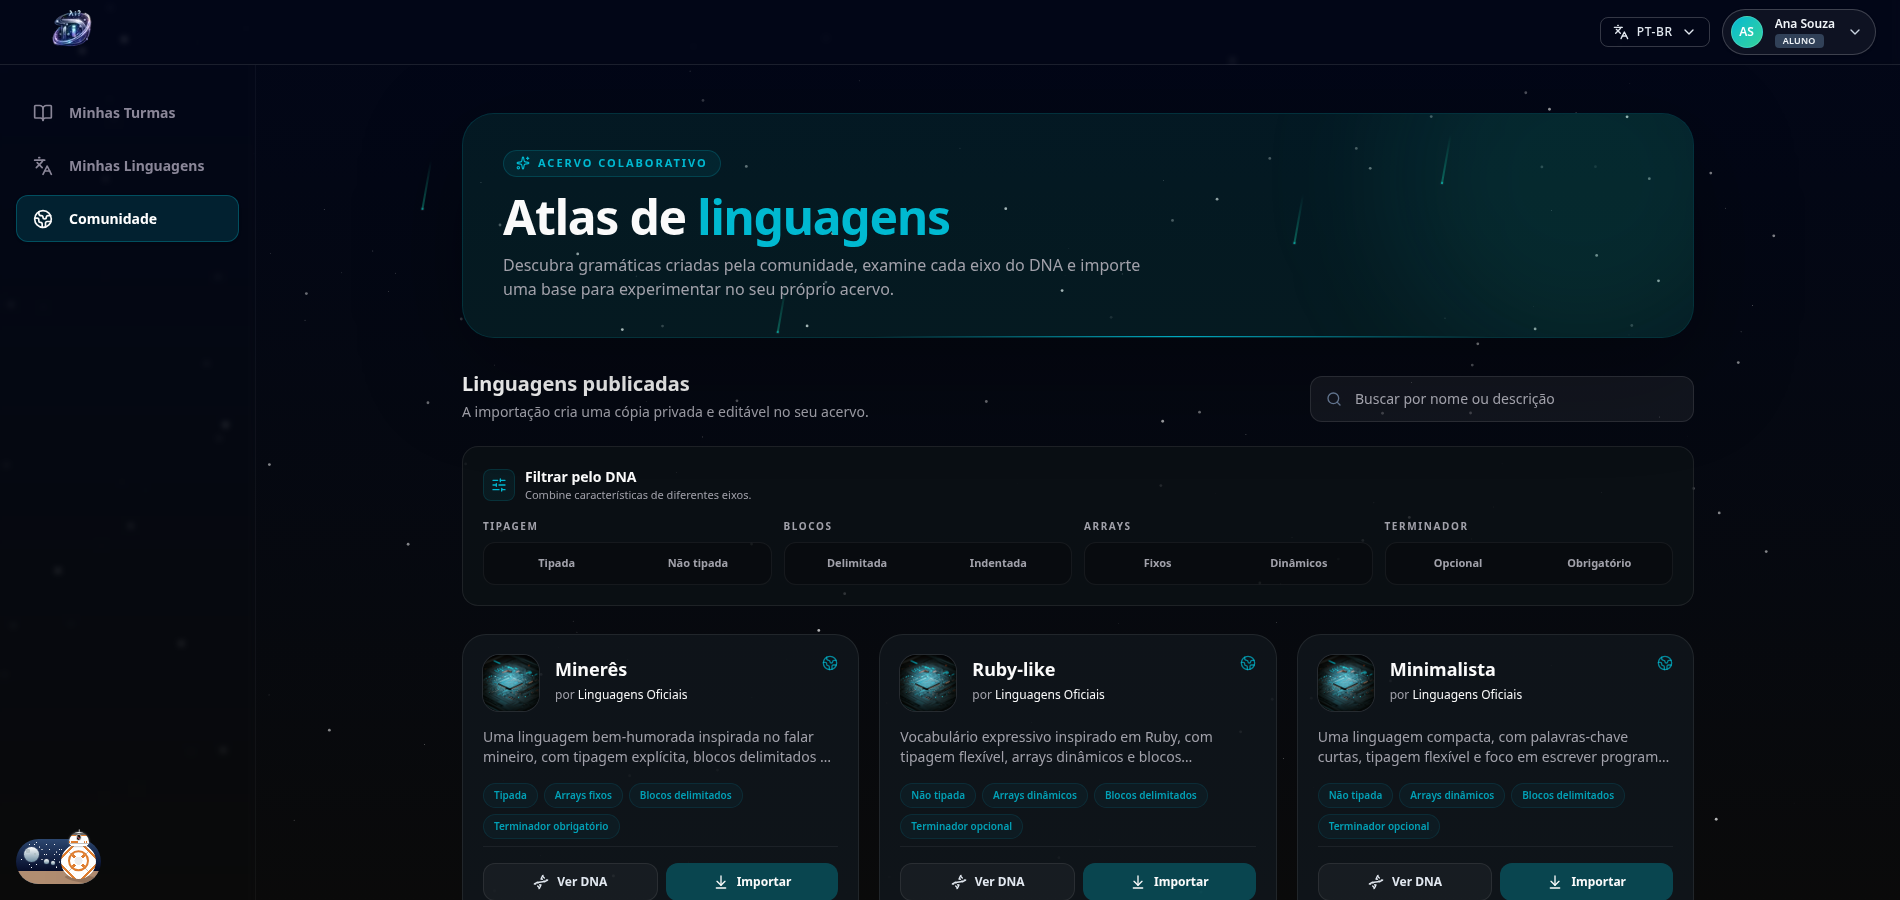
\includegraphics[width=\textwidth,height=0.34\textheight,keepaspectratio]{Linguagens/comunidade.png}
    \caption{Catálogo de linguagens da comunidade, com filtros e importação.}
    \label{fig:comunidade}
    \legend{Fonte: elaborado pelo autor.}
\end{figure}

\subsection{Depuração e mensagens de erro (RF13 e RF14)}

A depuração passo a passo fica no painel lateral da IDE. O usuário marca pontos de parada pela margem do editor e inicia a sessão; a execução para no ponto marcado, a linha em processamento fica destacada e o painel mostra as variáveis com seus valores e tipos e a pilha de chamadas. Os botões do painel continuam a execução, avançam uma instrução, entram e saem de chamadas, reiniciam e encerram a sessão (Figura~\ref{fig:depuracao}). Na captura, a execução está parada no ponto da linha 6, dentro do laço, com \texttt{soma} igual a 0 e \texttt{i} igual a 1.

\begin{figure}[H]
    \centering
    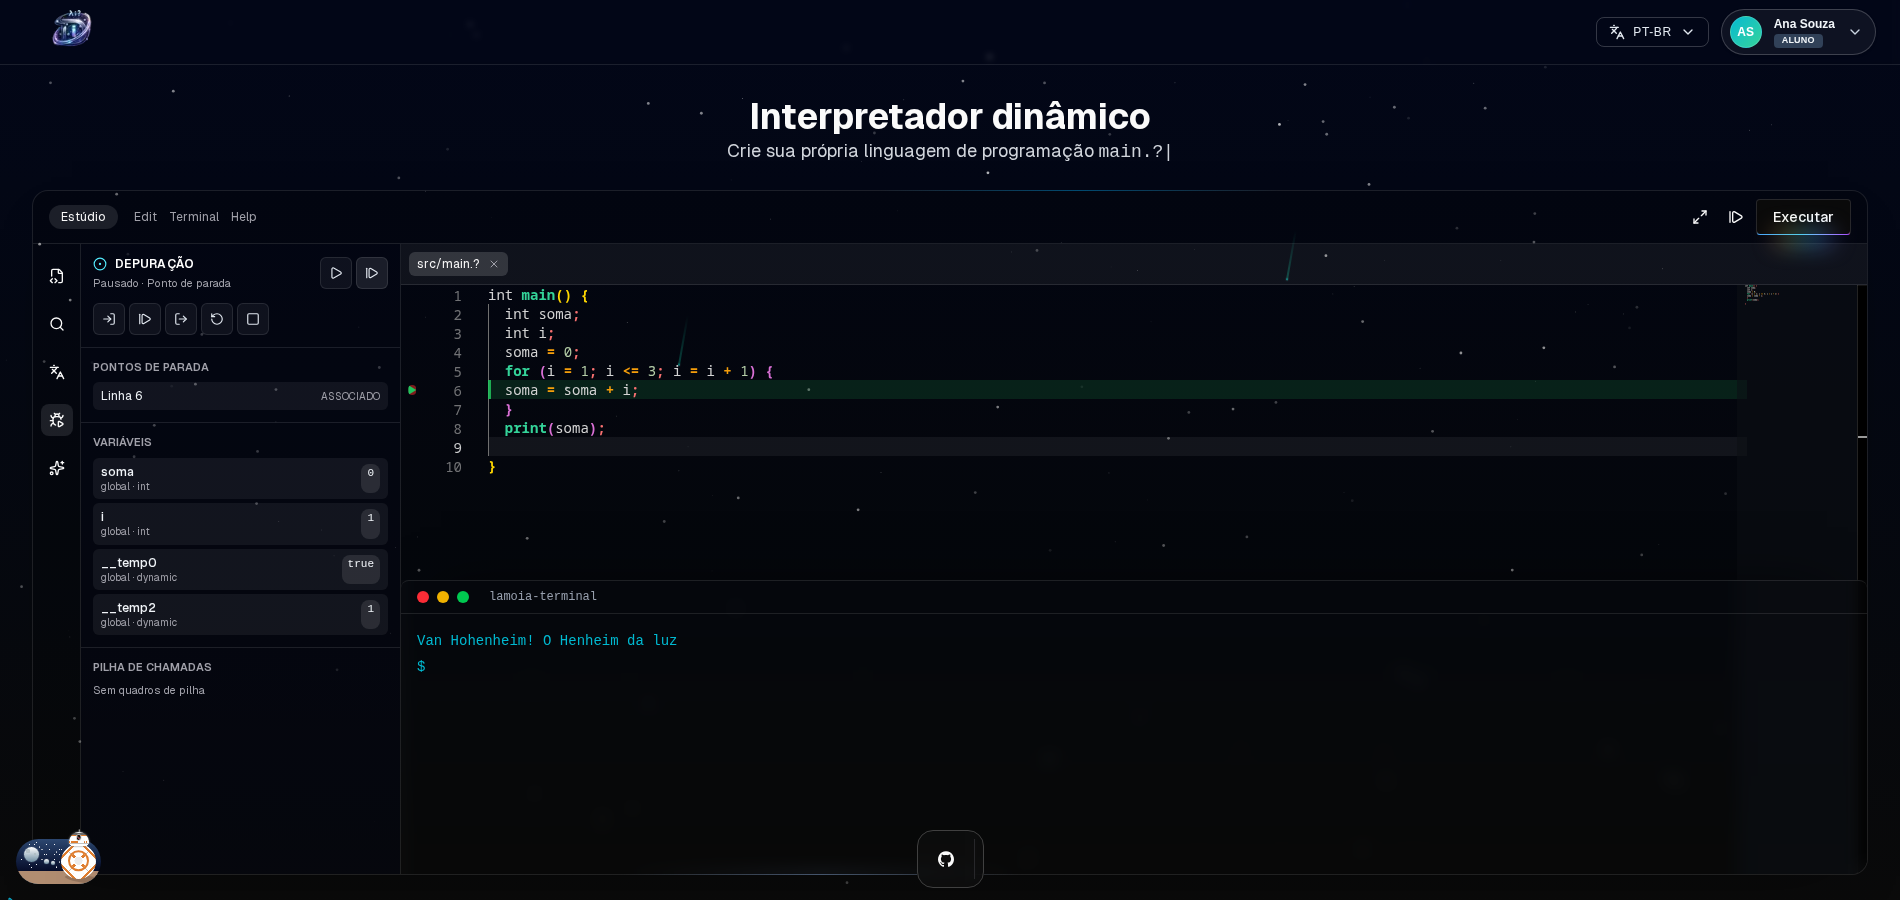
\includegraphics[width=\textwidth,height=0.34\textheight,keepaspectratio]{IDE/depuracao.png}
    \caption{Depuração passo a passo, com a execução parada em um ponto de parada e as variáveis no painel lateral.}
    \label{fig:depuracao}
    \legend{Fonte: elaborado pelo autor.}
\end{figure}

Quando o programa tem um erro, a mensagem aparece no editor, sob a linha em que o problema foi encontrado, e também em uma notificação. Na Figura~\ref{fig:erro-sintaxe}, falta o ponto e vírgula depois de \texttt{total = 10}, e a mensagem indica a linha e a coluna, o que era esperado (``final de instrução'') e o que foi encontrado, com a classe do \textit{token} e o lexema escrito. A classe aparece pelo nome canônico (``palavra reservada print'') e o lexema, pela palavra digitada; com uma linguagem personalizada, a mensagem mostra a palavra do usuário apenas no lexema, de modo que o RF14 é atendido em parte.

\begin{figure}[H]
    \centering
    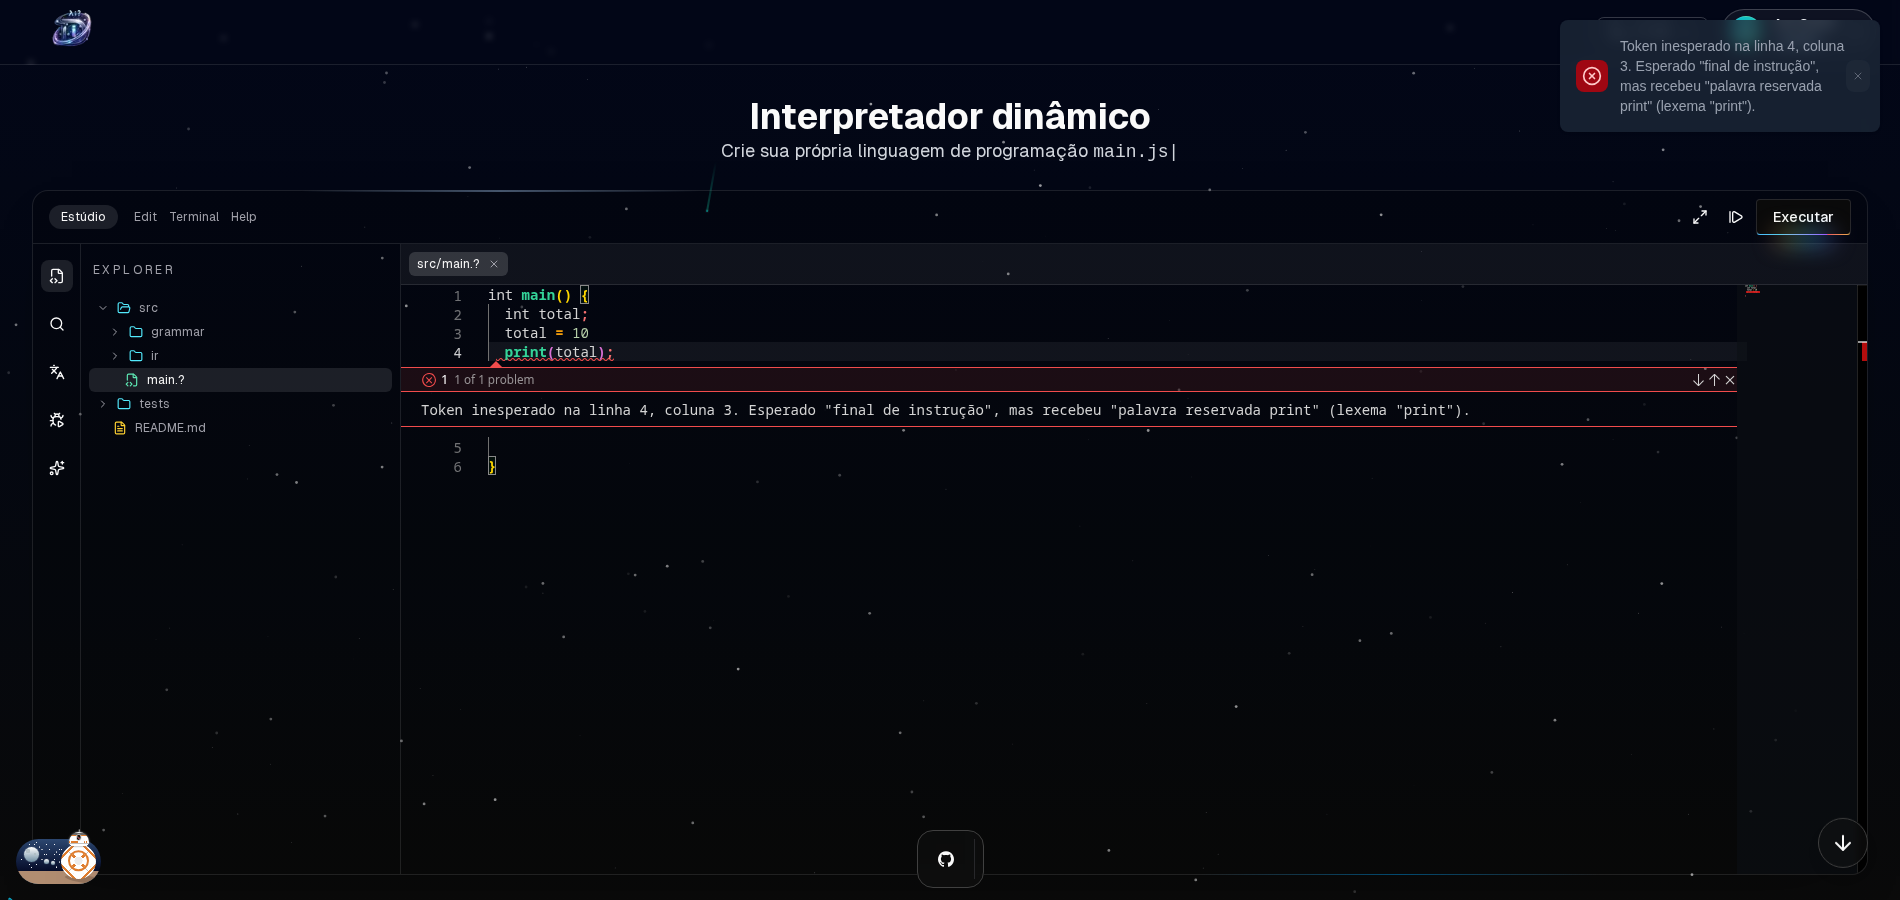
\includegraphics[width=\textwidth,height=0.34\textheight,keepaspectratio]{IDE/erro_sintaxe.png}
    \caption{Mensagem de erro sintático exibida no editor e em notificação.}
    \label{fig:erro-sintaxe}
    \legend{Fonte: elaborado pelo autor.}
\end{figure}

\subsection{Gestão e consulta de turmas (RF15)}

O painel do professor mostra as turmas sob sua responsabilidade, cada uma com a descrição, o código de acesso e o número de exercícios, e tem o botão para criar uma nova turma. Pelo menu lateral, o professor chega também aos seus exercícios e às suas listas. A Figura~\ref{fig:painel-professor} mostra esse painel.

\begin{figure}[H]
    \centering
    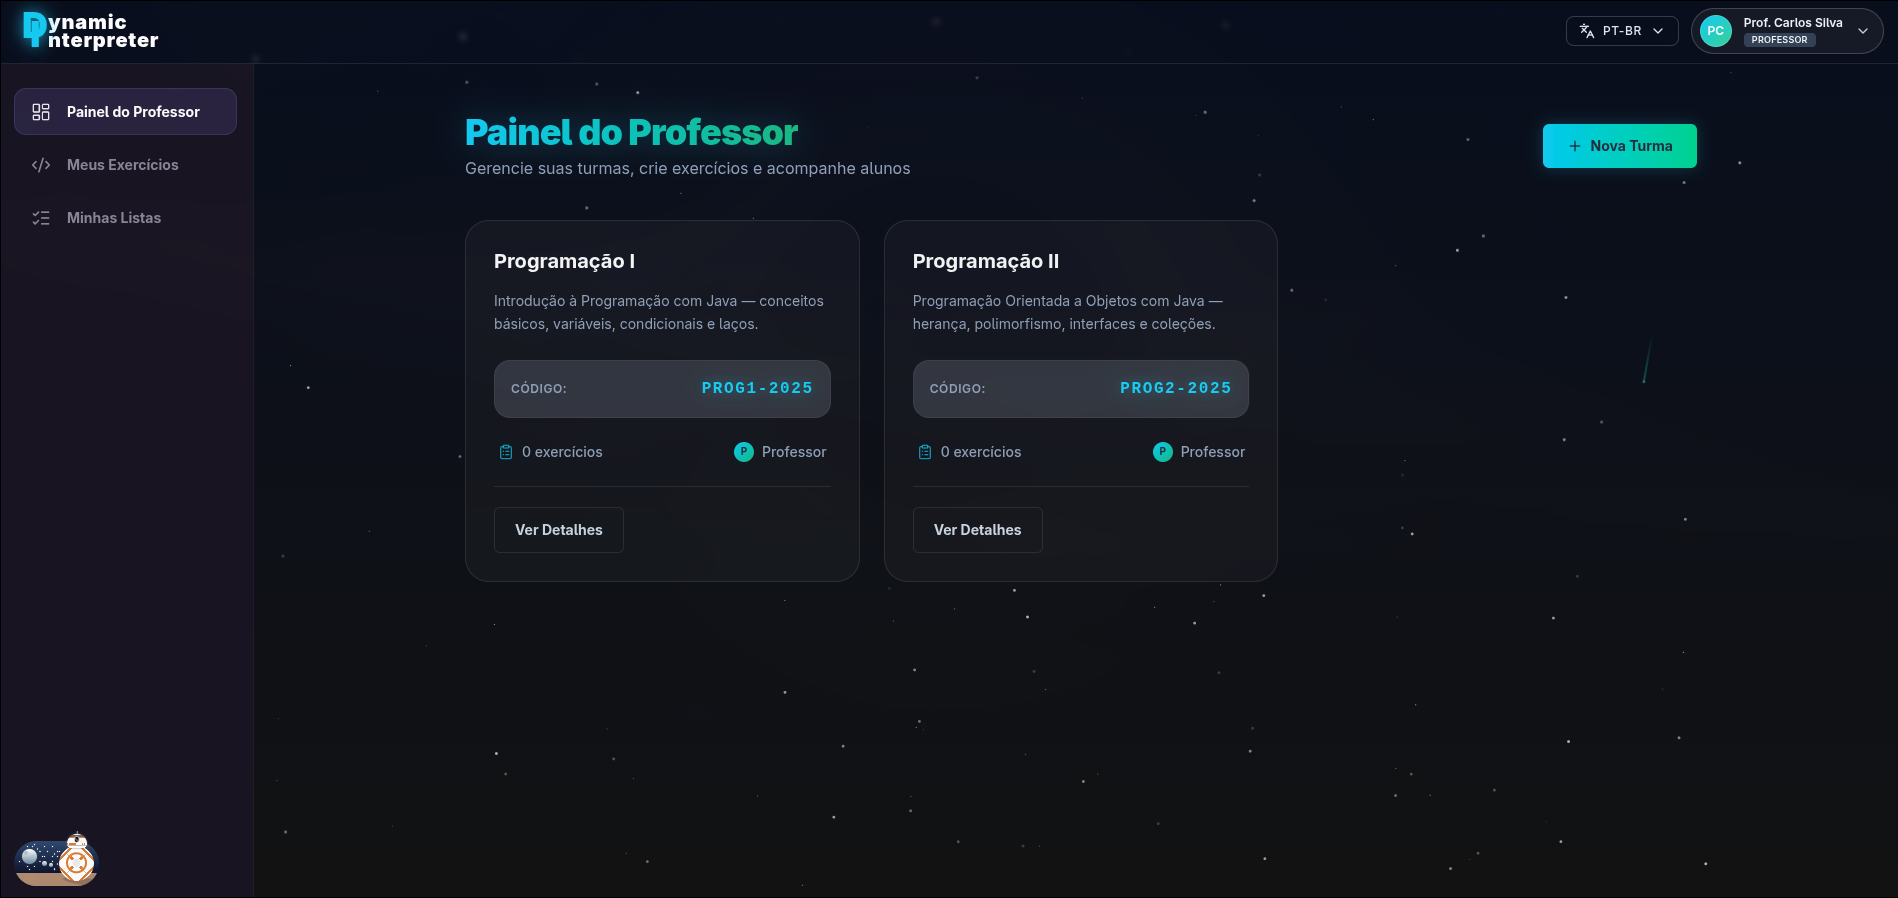
\includegraphics[width=\textwidth,height=0.34\textheight,keepaspectratio]{Professor/painel_professor.png}
    \caption{Painel principal do professor.}
    \label{fig:painel-professor}
    \legend{Fonte: elaborado pelo autor.}
\end{figure}

Ao abrir uma turma, o professor vê, na aba ``Todos da Turma'', o professor responsável, os estudantes matriculados com o número de exercícios concluídos por cada um e um quadro com o total de estudantes, o total de exercícios e a média de conclusões (Figura~\ref{fig:professor-turma}).

\begin{figure}[H]
    \centering
    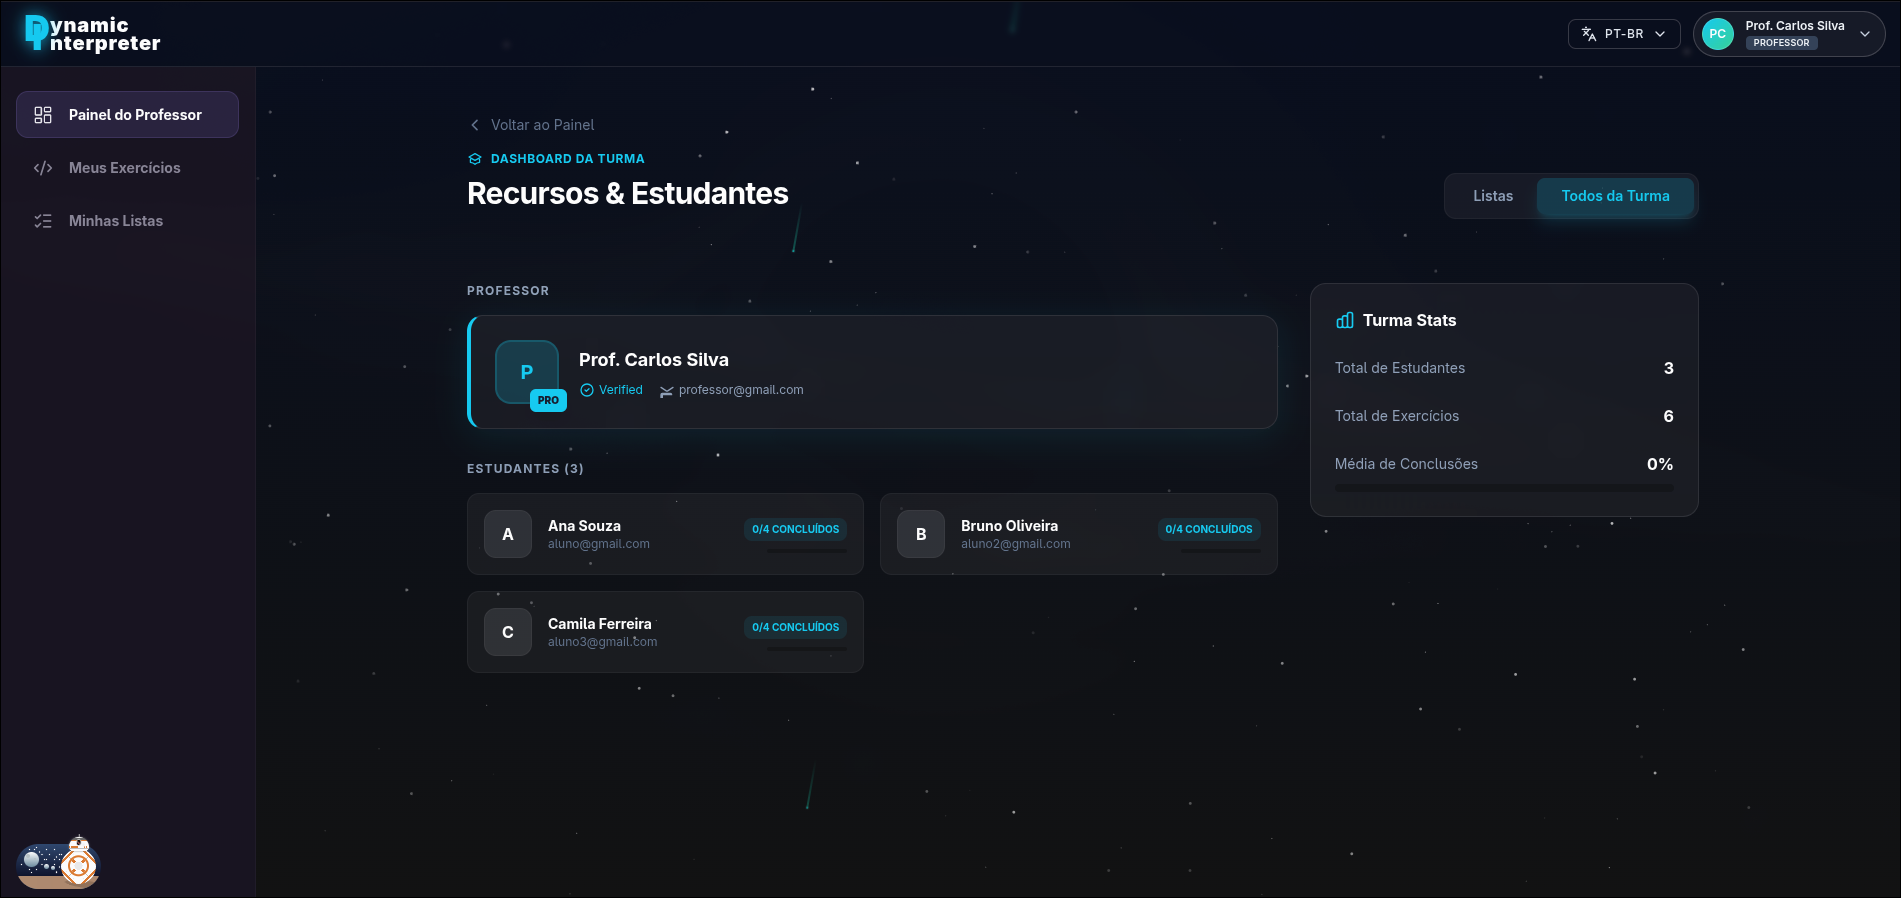
\includegraphics[width=\textwidth,height=0.34\textheight,keepaspectratio]{Professor/detail_turma.png}
    \caption{Turma vista pelo professor: participantes e estatísticas.}
    \label{fig:professor-turma}
    \legend{Fonte: elaborado pelo autor.}
\end{figure}

A aba ``Listas'' da mesma tela mostra as listas publicadas para a turma, com o número de exercícios, o mínimo exigido e o prazo (Figura~\ref{fig:professor-listas-turma}).

\begin{figure}[H]
    \centering
    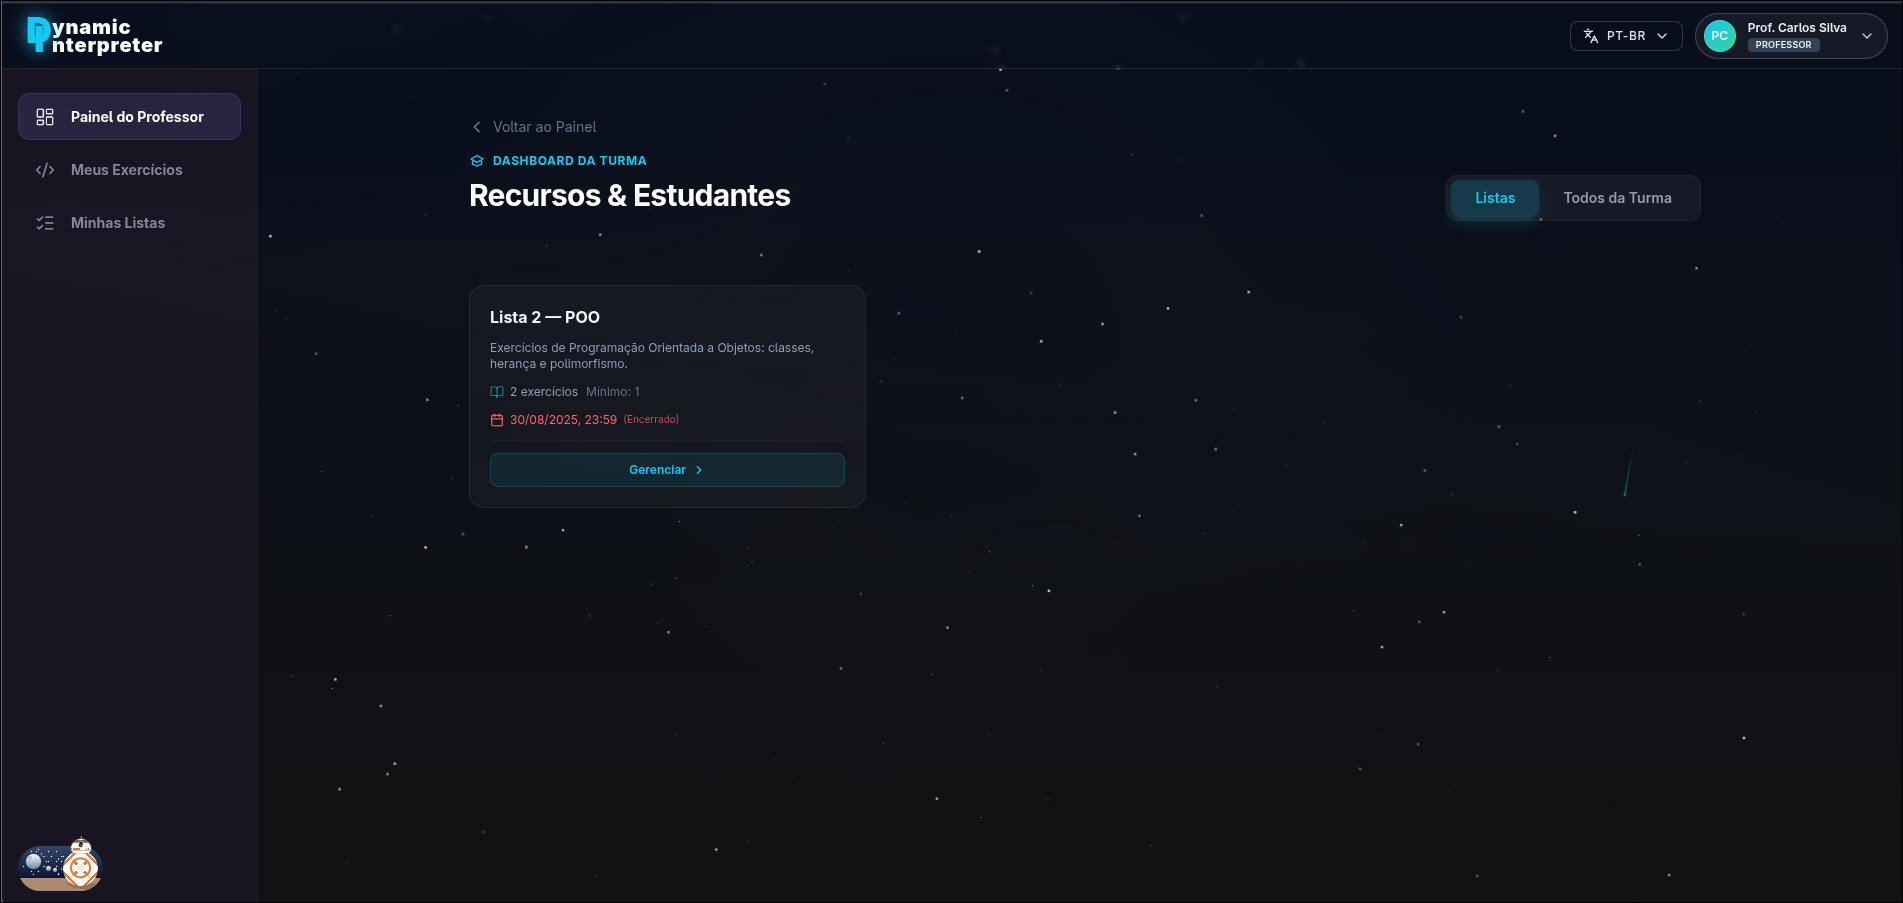
\includegraphics[width=\textwidth,height=0.34\textheight,keepaspectratio]{Professor/listas_turma.png}
    \caption{Listas de exercícios vinculadas à turma, na visão do professor.}
    \label{fig:professor-listas-turma}
    \legend{Fonte: elaborado pelo autor.}
\end{figure}

Do lado do aluno, o painel ``Minhas Turmas'' mostra as turmas em que o estudante está matriculado e um cartão para entrar em uma nova turma com o código fornecido pelo professor (Figura~\ref{fig:painel-aluno}).

\begin{figure}[H]
    \centering
    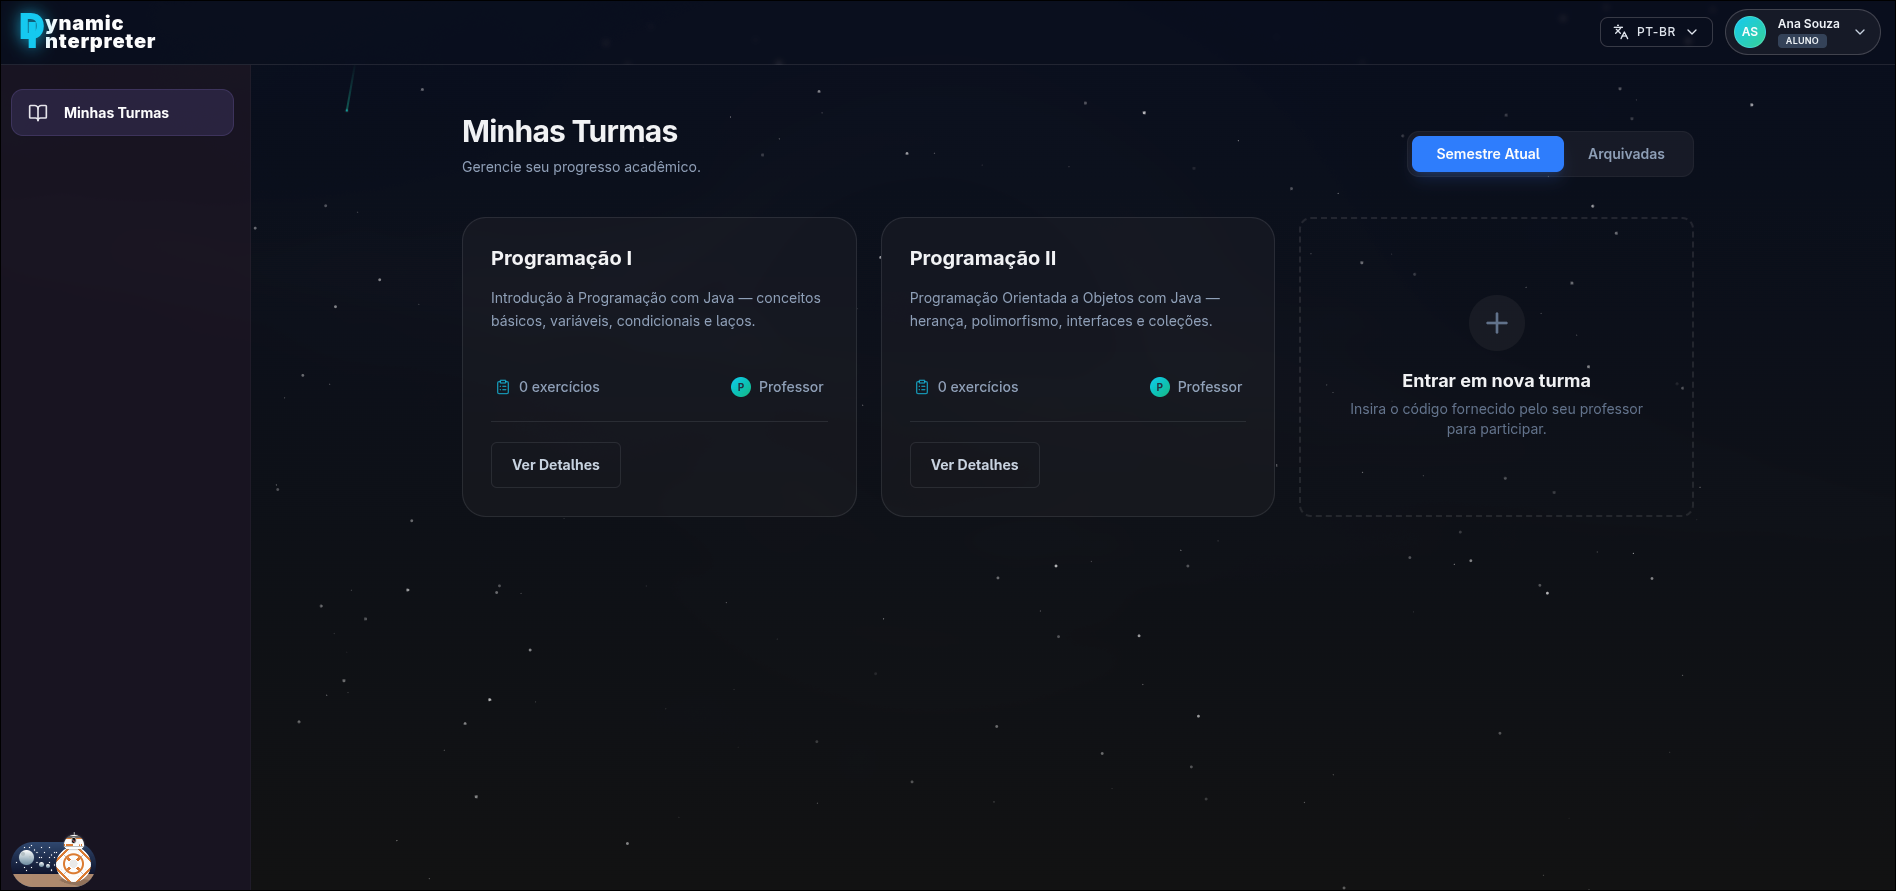
\includegraphics[width=\textwidth,height=0.34\textheight,keepaspectratio]{Aluno/painel_aluno.png}
    \caption{Painel principal do aluno, com as turmas e a entrada em nova turma.}
    \label{fig:painel-aluno}
    \legend{Fonte: elaborado pelo autor.}
\end{figure}

Ao abrir uma turma, o aluno vê a mesma organização em abas da tela do professor. Na aba ``Todos da Turma'' aparecem o professor responsável, os colegas matriculados com o número de exercícios concluídos por cada um e os totais da turma (Figura~\ref{fig:aluno-turma}); a aba ``Listas'' mostra as listas publicadas, apresentadas mais adiante na Figura~\ref{fig:aluno-listas}.

\begin{figure}[H]
    \centering
    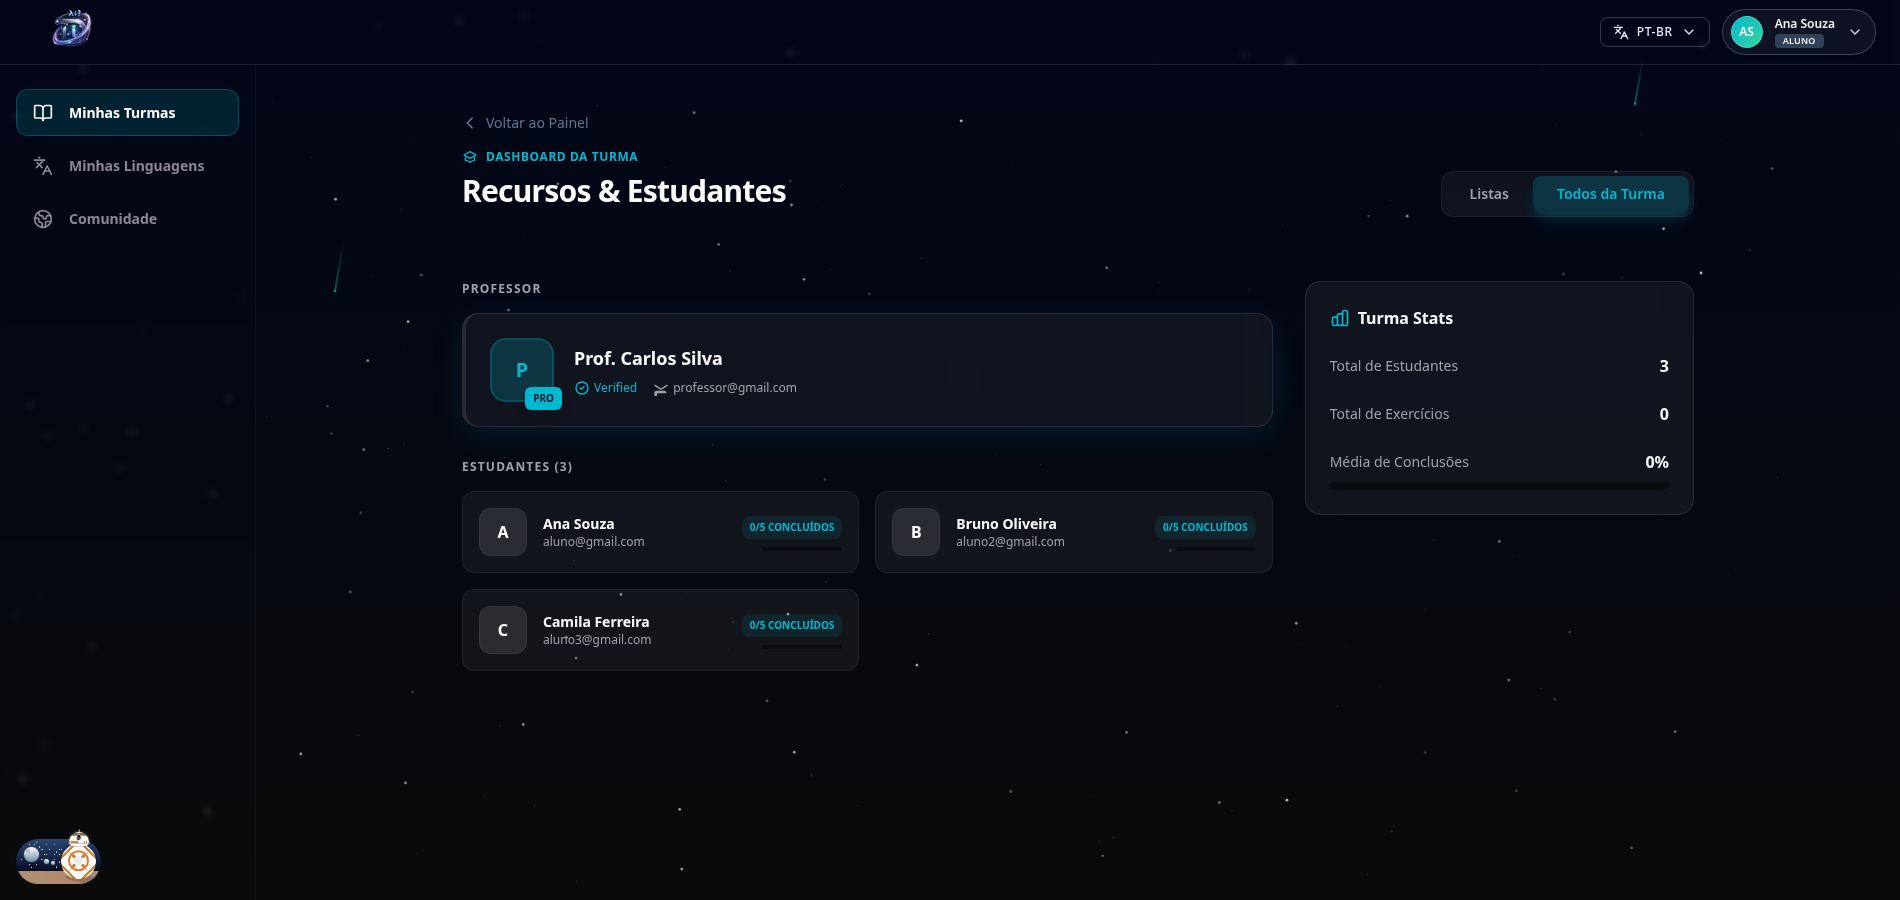
\includegraphics[width=\textwidth,height=0.34\textheight,keepaspectratio]{Aluno/detail_turma.png}
    \caption{Detalhe de uma turma visto pelo aluno.}
    \label{fig:aluno-turma}
    \legend{Fonte: elaborado pelo autor.}
\end{figure}

\subsection{Gestão de exercícios, listas e submissões (RF16 a RF20)}

Os exercícios do professor ficam na tela ``Meus Exercícios'', que mostra os enunciados existentes, o total de exercícios e de casos de teste e um campo de busca (Figura~\ref{fig:prof-exec-list}).

\begin{figure}[H]
    \centering
    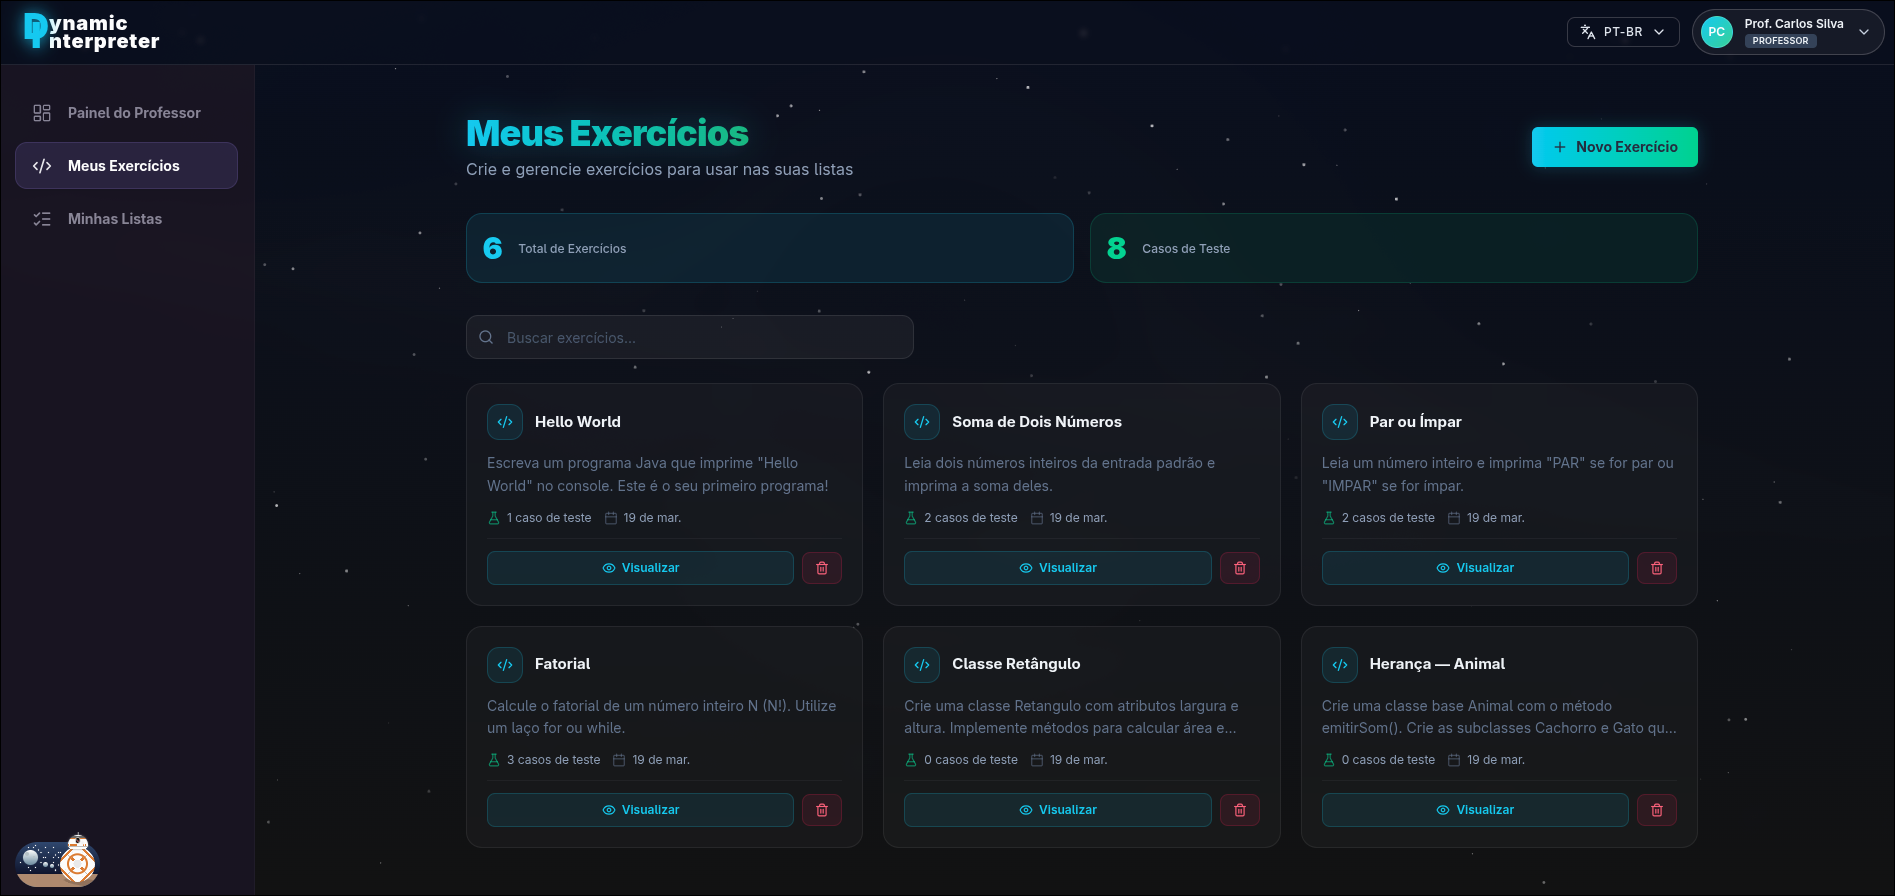
\includegraphics[width=\textwidth,height=0.34\textheight,keepaspectratio]{Professor/Exercicios/list.png}
    \caption{Listagem dos exercícios do professor.}
    \label{fig:prof-exec-list}
    \legend{Fonte: elaborado pelo autor.}
\end{figure}

A tela de criação reúne em um formulário a descrição do problema, os casos de teste com entradas e saídas esperadas e a vinculação a uma configuração de linguagem que delimita o vocabulário disponível ao aluno (Figura~\ref{fig:prof-exec-create}).

\begin{figure}[H]
    \centering
    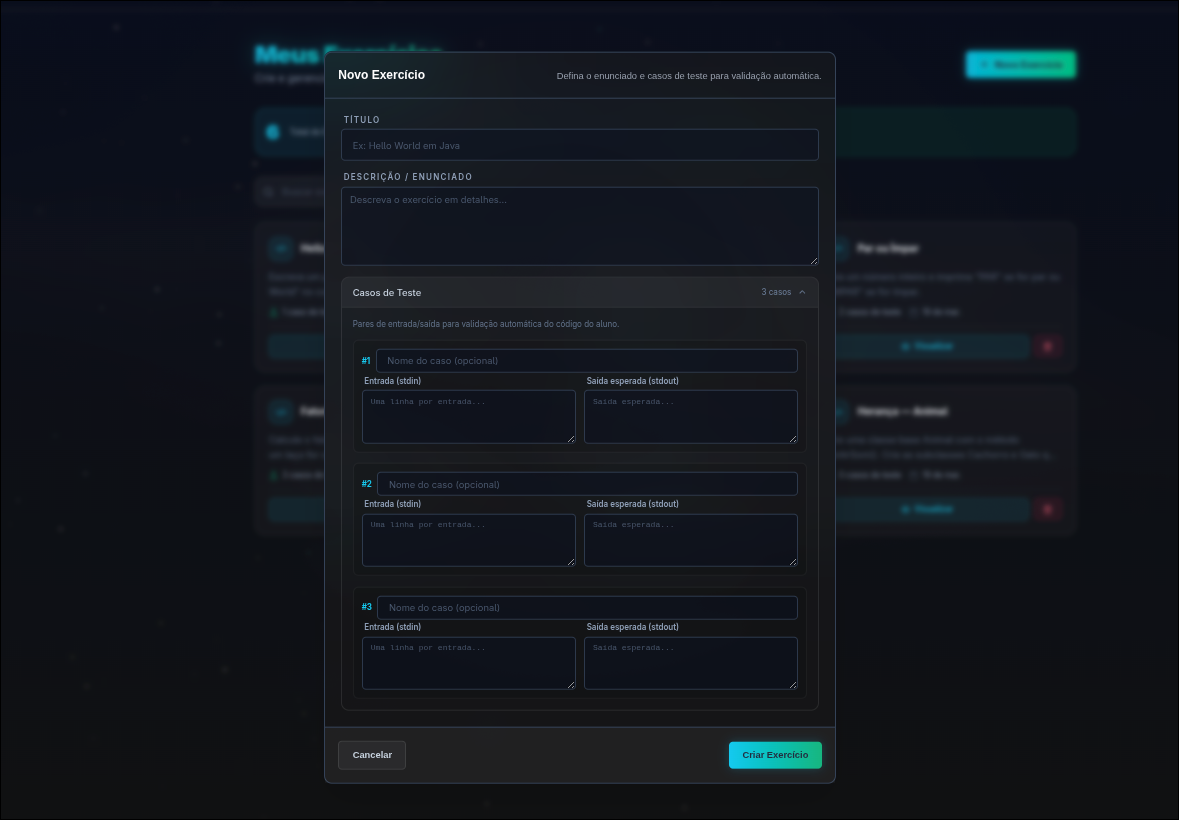
\includegraphics[width=\textwidth,height=0.34\textheight,keepaspectratio]{Professor/Exercicios/create.png}
    \caption{Criação de um novo exercício pelo professor.}
    \label{fig:prof-exec-create}
    \legend{Fonte: elaborado pelo autor.}
\end{figure}

Depois de criado, o exercício pode ser aberto em uma janela de detalhe, com o enunciado e os casos de teste cadastrados (Figura~\ref{fig:prof-exec-detail}).

\begin{figure}[H]
    \centering
    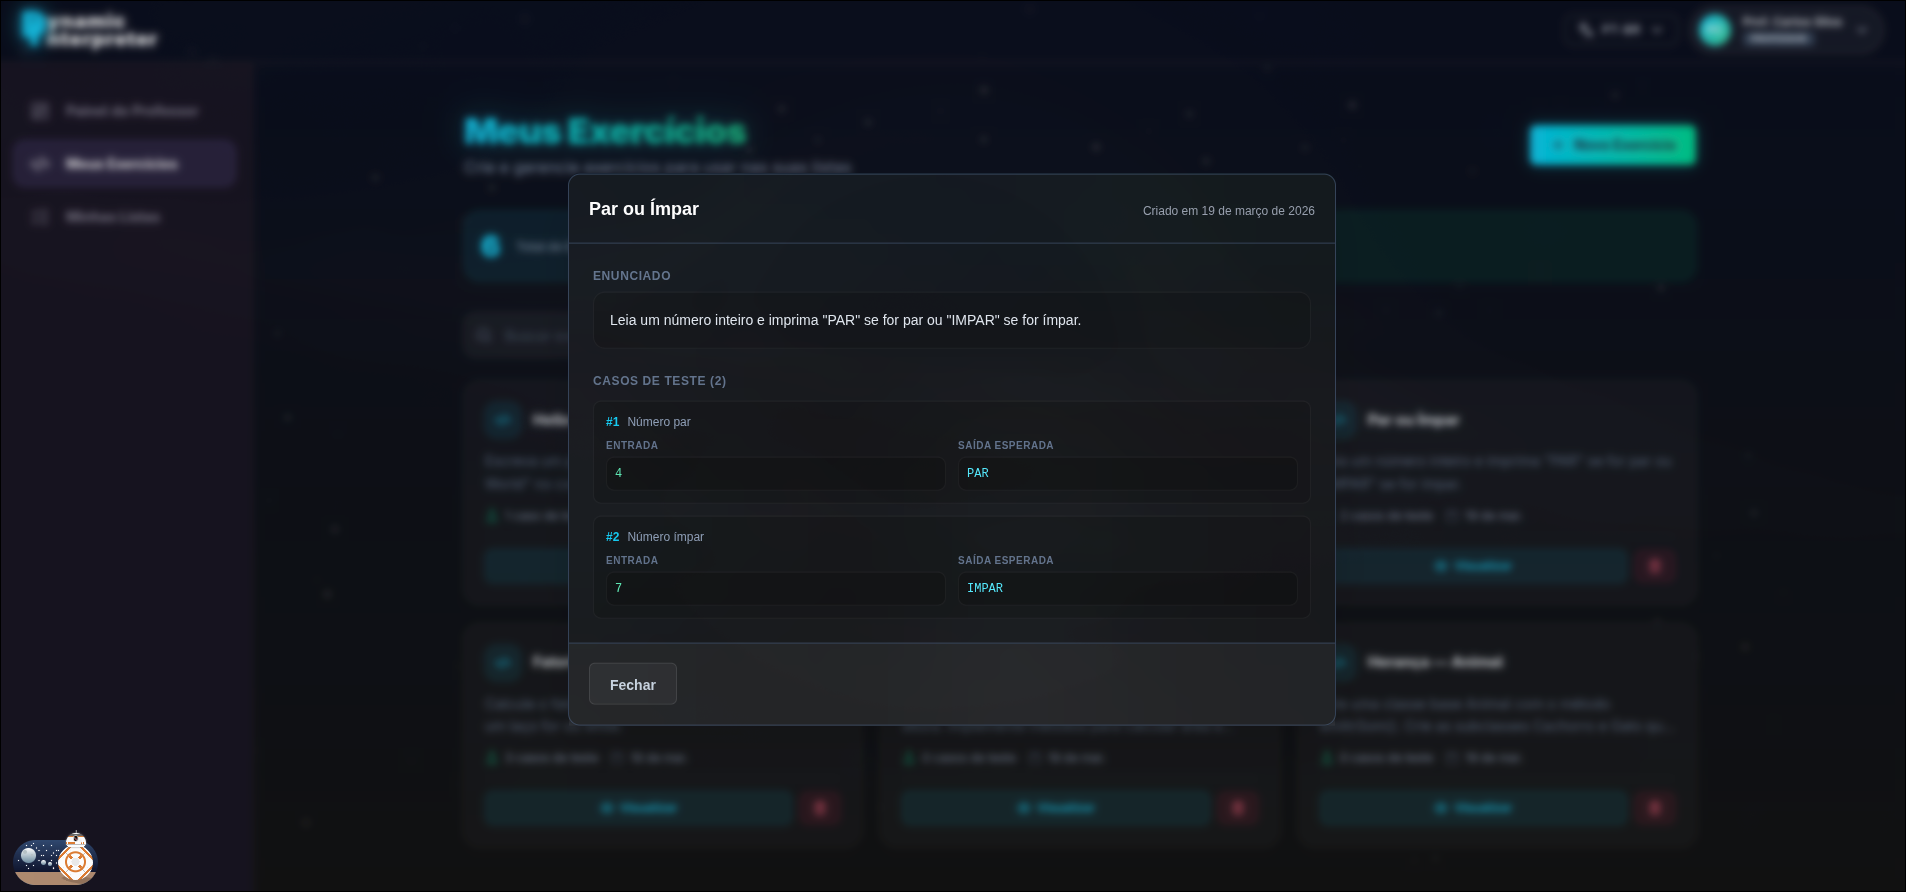
\includegraphics[width=\textwidth,height=0.34\textheight,keepaspectratio]{Professor/Exercicios/detail.png}
    \caption{Detalhamento de um exercício.}
    \label{fig:prof-exec-detail}
    \legend{Fonte: elaborado pelo autor.}
\end{figure}

Os exercícios são organizados em listas, na tela ``Minhas Listas'', que mostra as listas existentes com o número de exercícios e a turma de cada uma (Figura~\ref{fig:prof-lista-list}).

\begin{figure}[H]
    \centering
    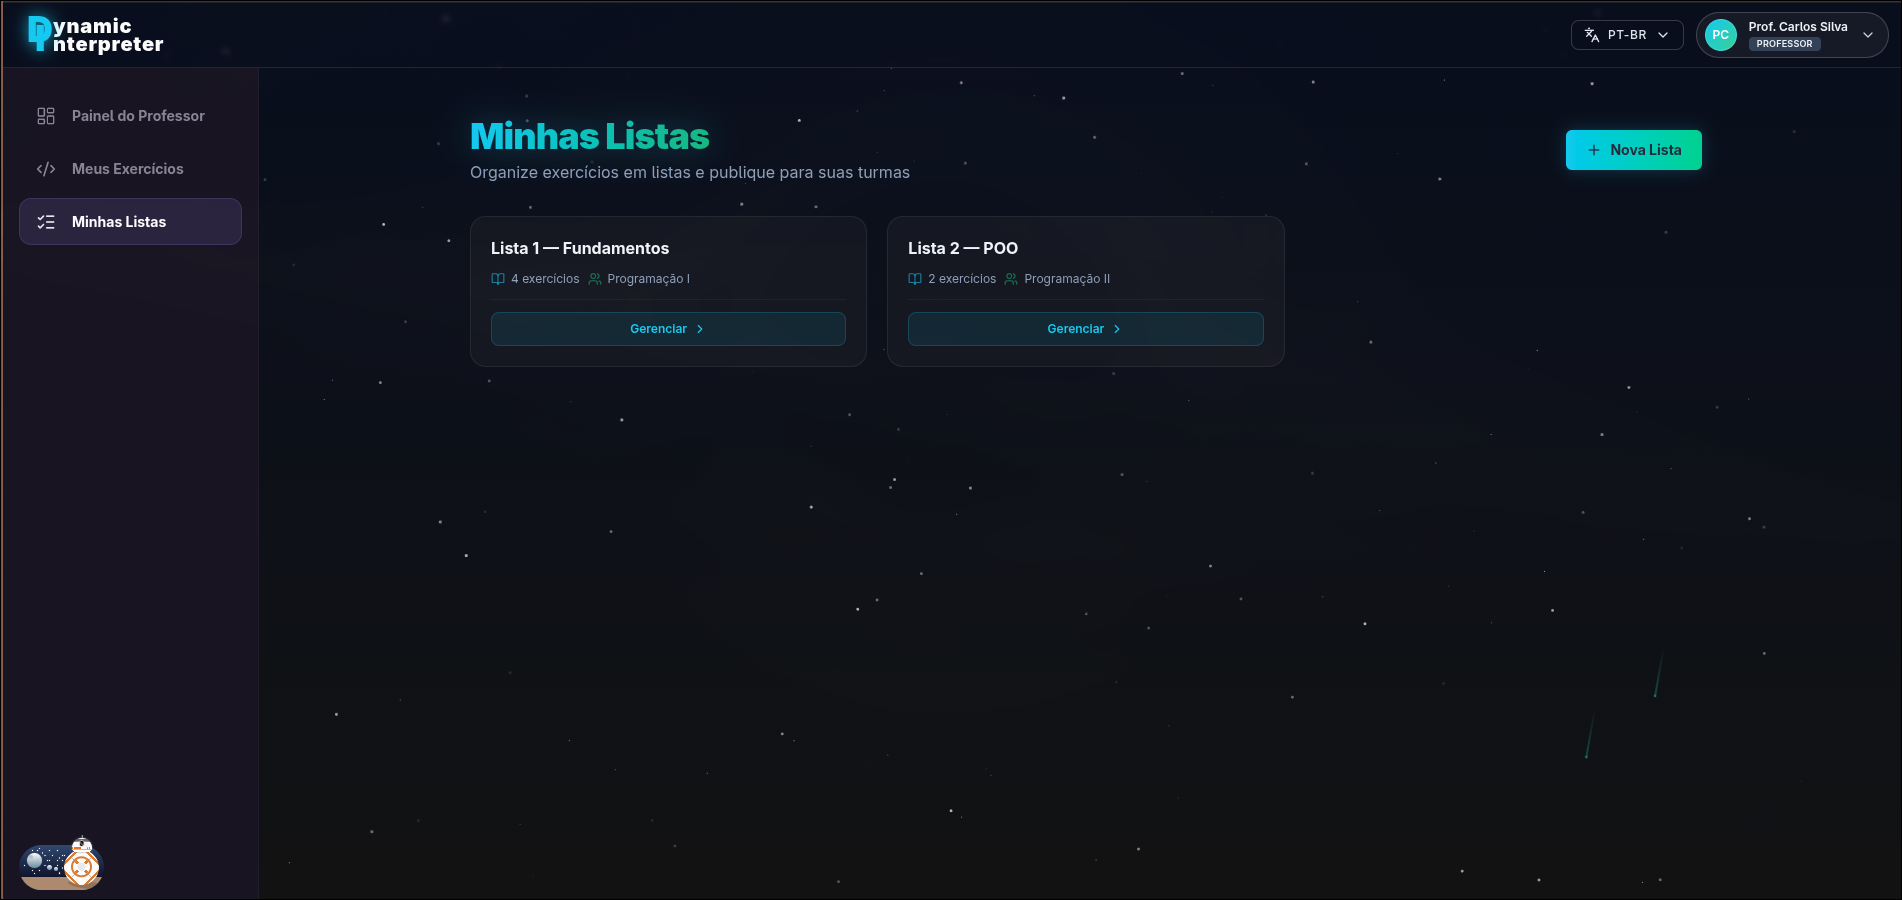
\includegraphics[width=\textwidth,height=0.34\textheight,keepaspectratio]{Professor/Listas/list.png}
    \caption{Listagem das listas de exercícios do professor.}
    \label{fig:prof-lista-list}
    \legend{Fonte: elaborado pelo autor.}
\end{figure}

O detalhe de uma lista reúne a linguagem obrigatória, os exercícios vinculados e as submissões recebidas (Figura~\ref{fig:prof-lista-config}).

\begin{figure}[H]
    \centering
    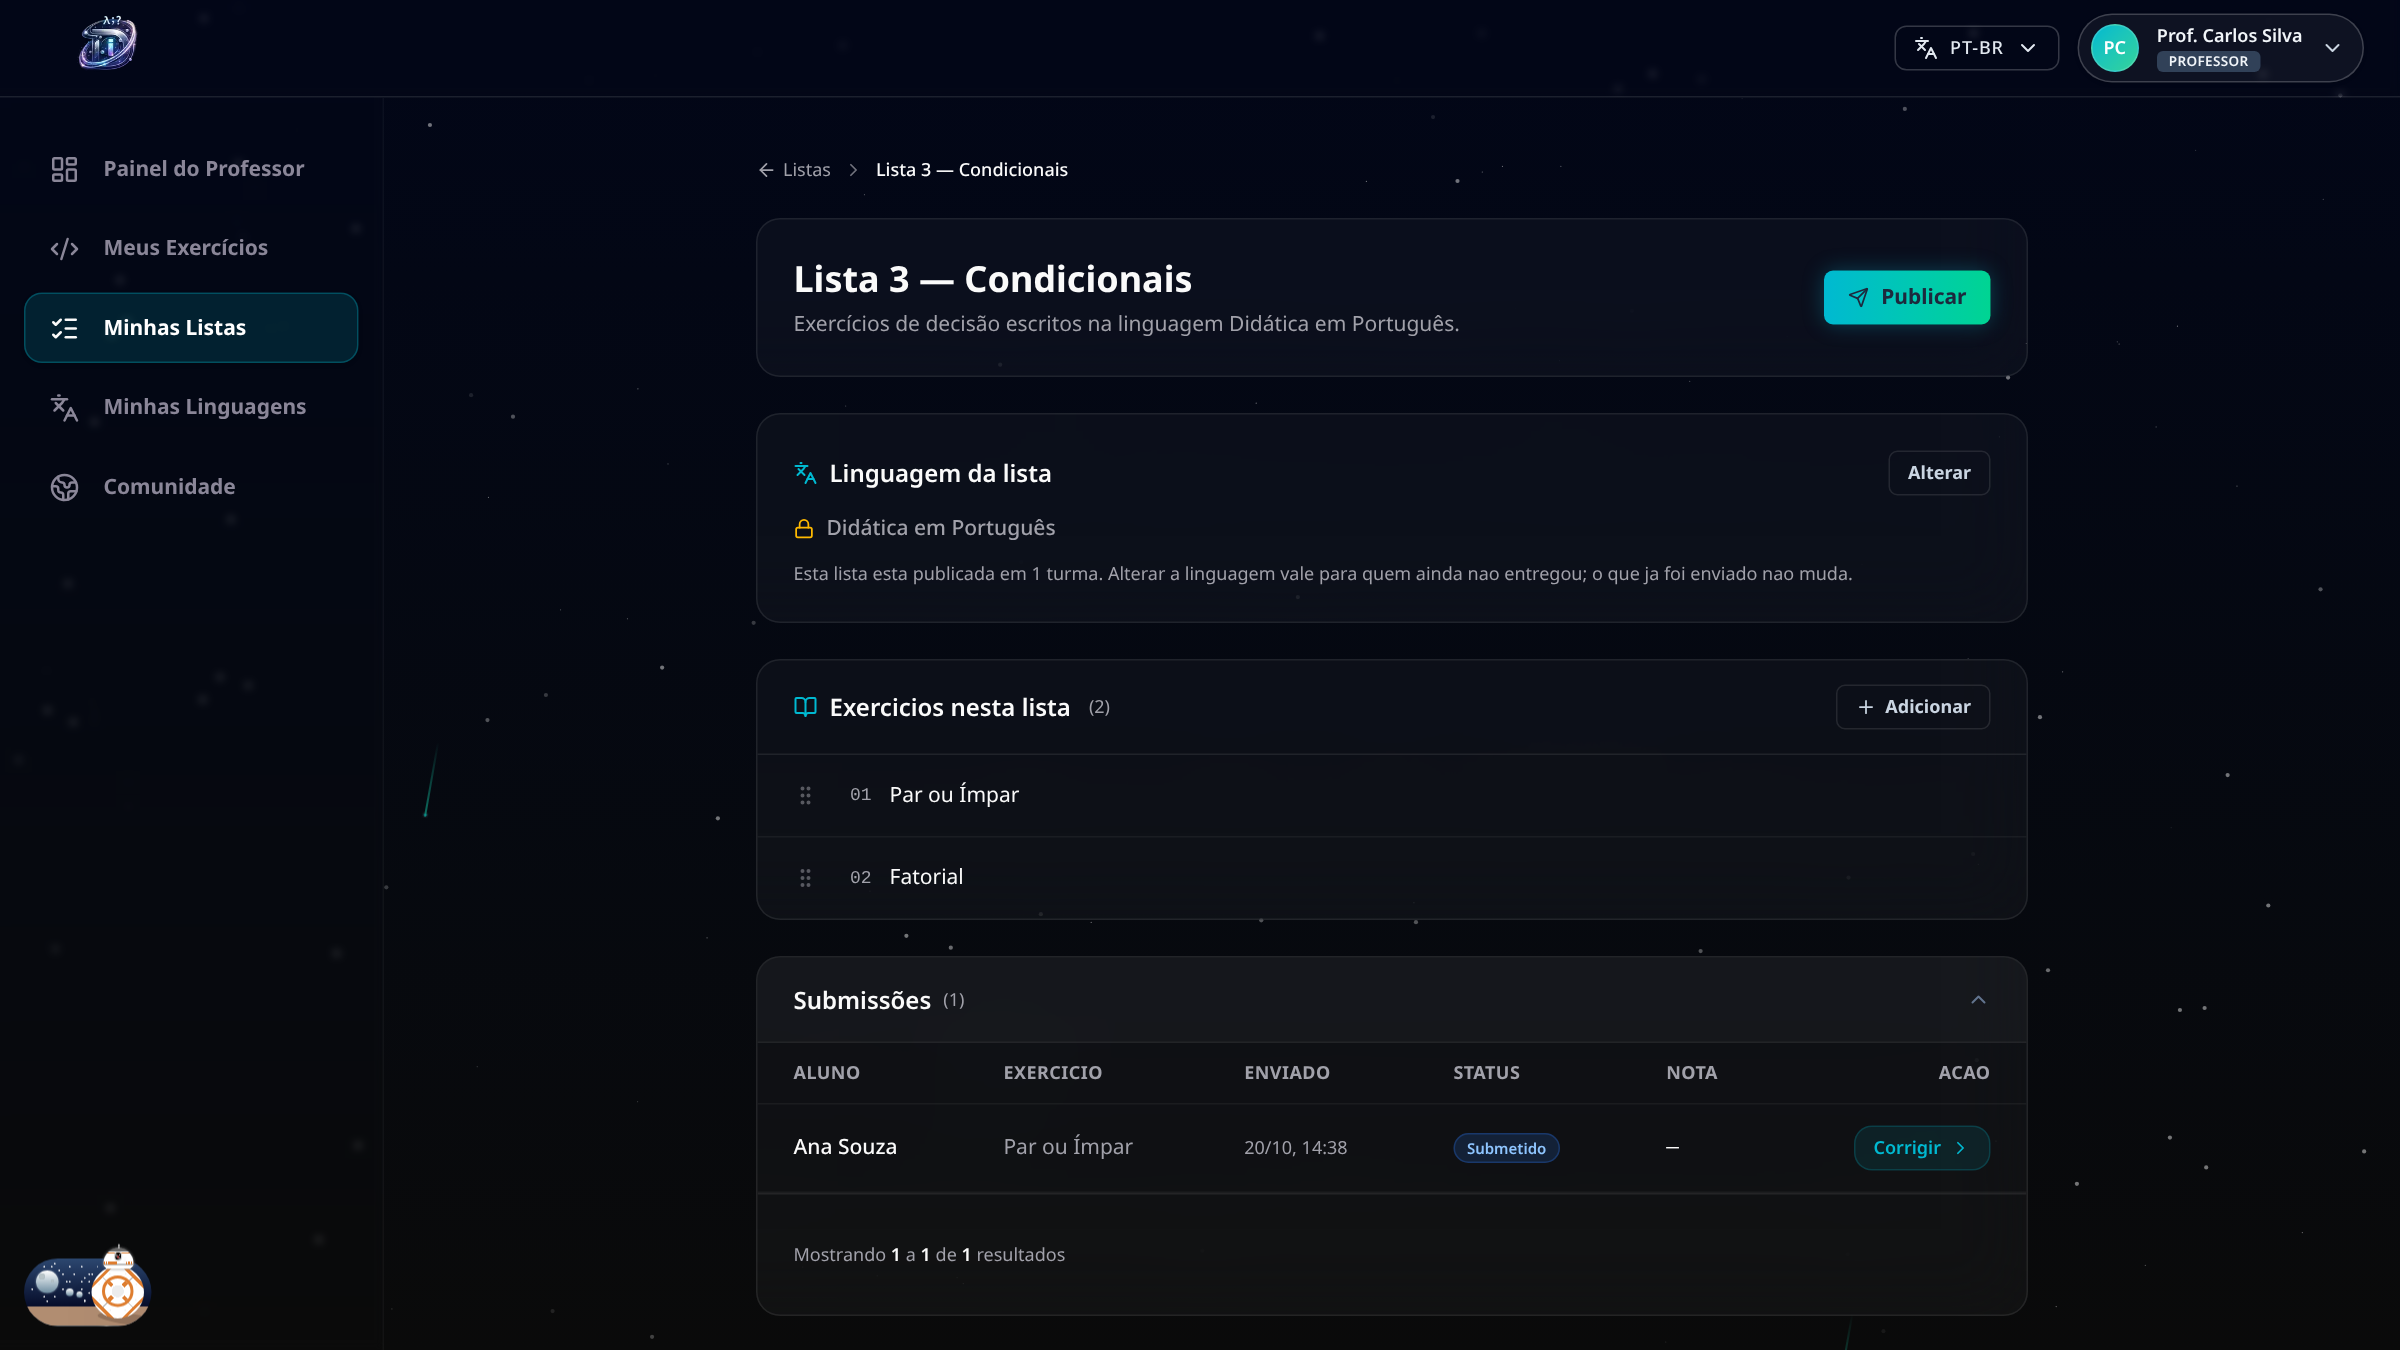
\includegraphics[width=\textwidth,height=0.34\textheight,keepaspectratio]{Professor/Listas/detalhe_lista.png}
    \caption{Detalhe de uma lista, com a linguagem obrigatória, os exercícios e as submissões.}
    \label{fig:prof-lista-config}
    \legend{Fonte: elaborado pelo autor.}
\end{figure}

Os exercícios são vinculados à lista por um utilitário de busca e seleção (Figura~\ref{fig:prof-lista-add}).

\begin{figure}[H]
    \centering
    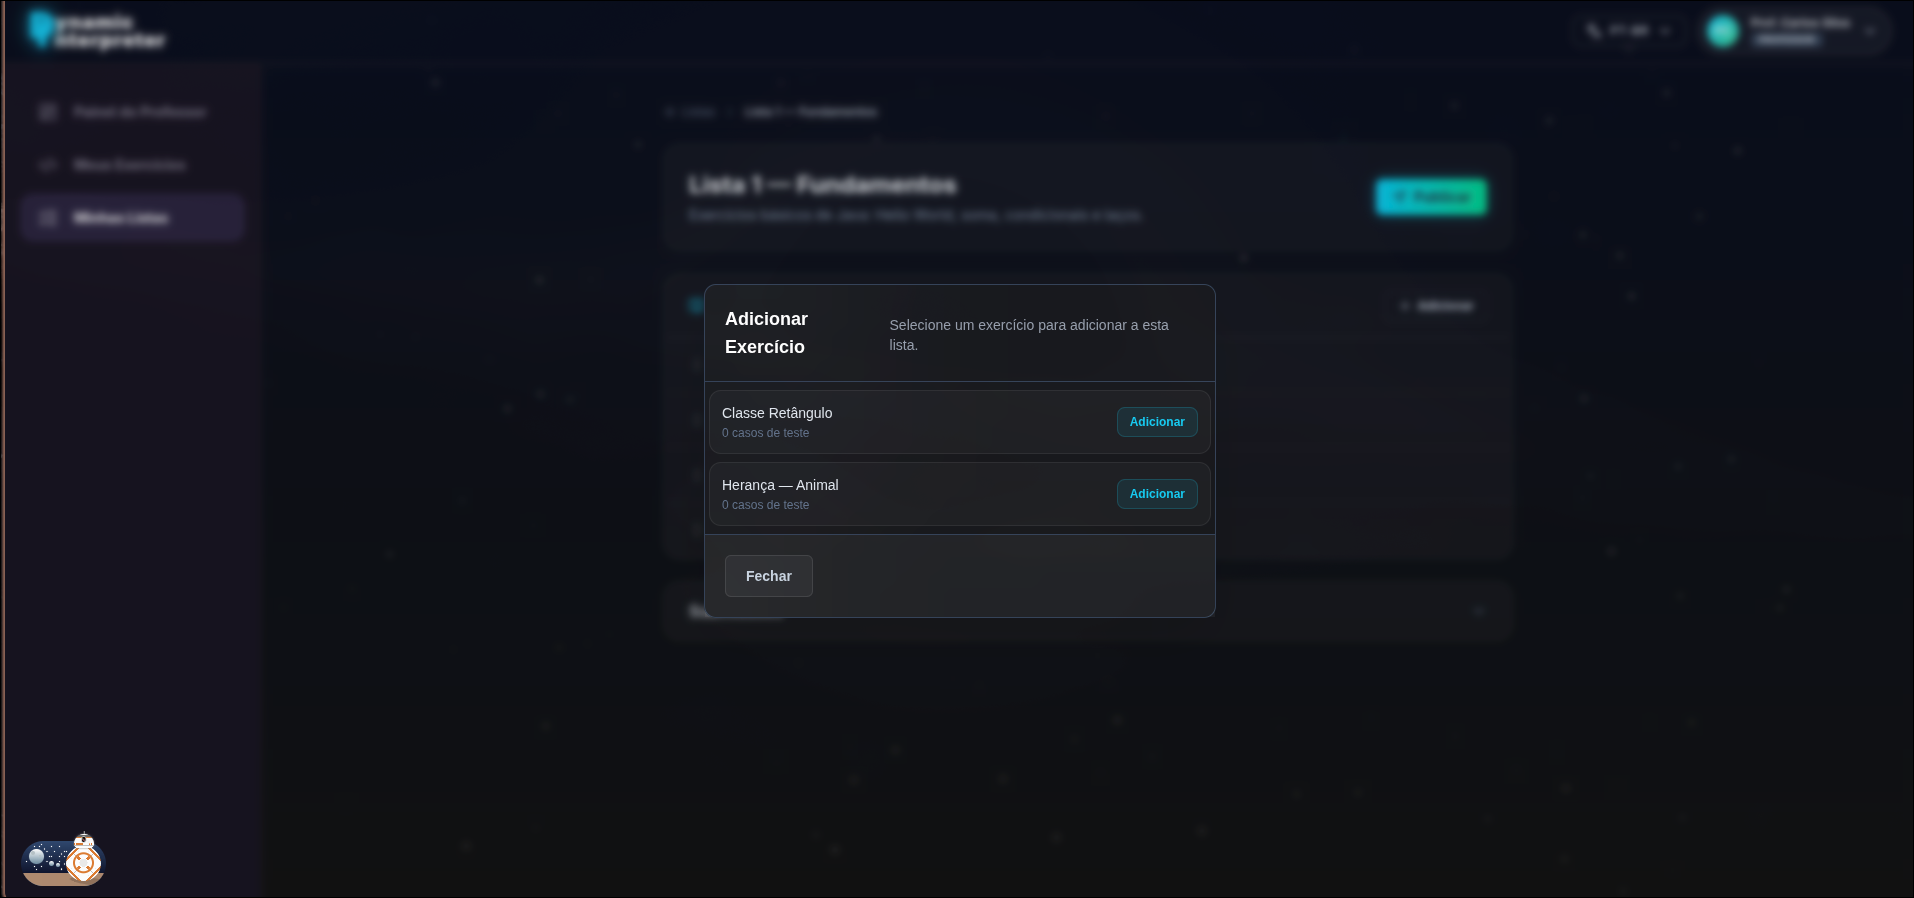
\includegraphics[width=\textwidth,height=0.34\textheight,keepaspectratio]{Professor/Listas/add_exec.png}
    \caption{Vinculação de exercícios a uma lista.}
    \label{fig:prof-lista-add}
    \legend{Fonte: elaborado pelo autor.}
\end{figure}

Por fim, a lista é publicada para a turma escolhida (Figura~\ref{fig:prof-lista-publish}).

\begin{figure}[H]
    \centering
    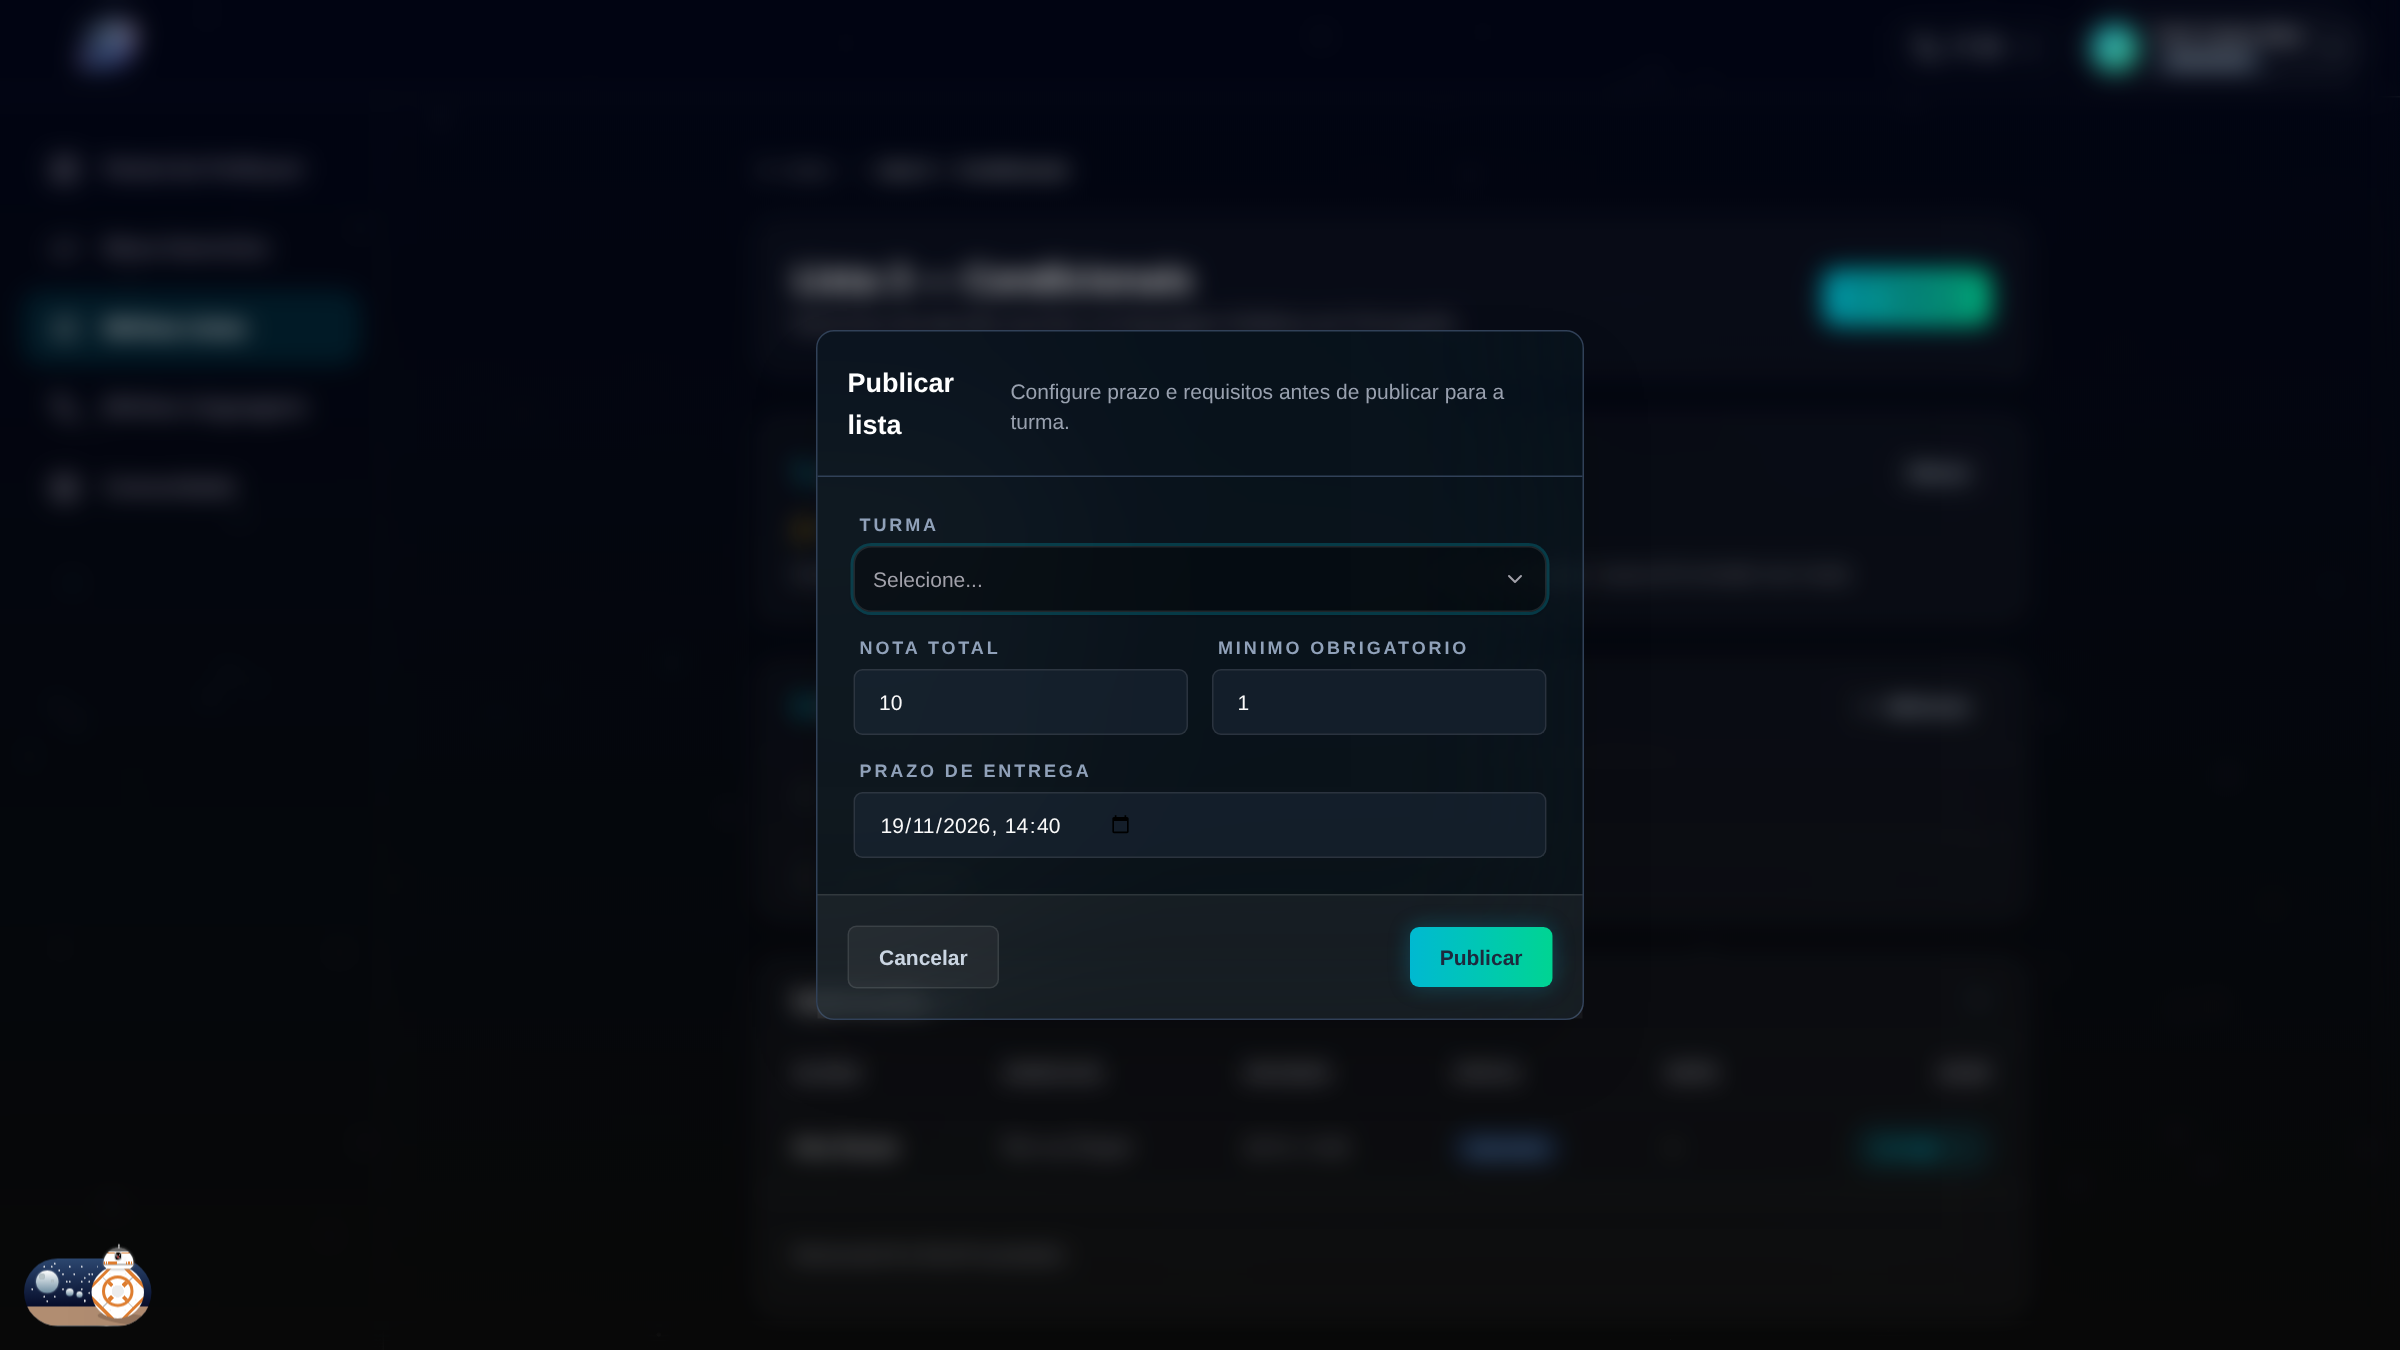
\includegraphics[width=\textwidth,height=0.34\textheight,keepaspectratio]{Professor/Listas/publicar_lista.png}
    \caption{Publicação de uma lista para a turma.}
    \label{fig:prof-lista-publish}
    \legend{Fonte: elaborado pelo autor.}
\end{figure}

Depois de publicada, a lista aparece para o aluno na tela da turma. Cada lista mostra o estado (na captura, não iniciada), o número mínimo de exercícios, o prazo e o progresso em exercícios concluídos (Figura~\ref{fig:aluno-listas}).

\begin{figure}[H]
    \centering
    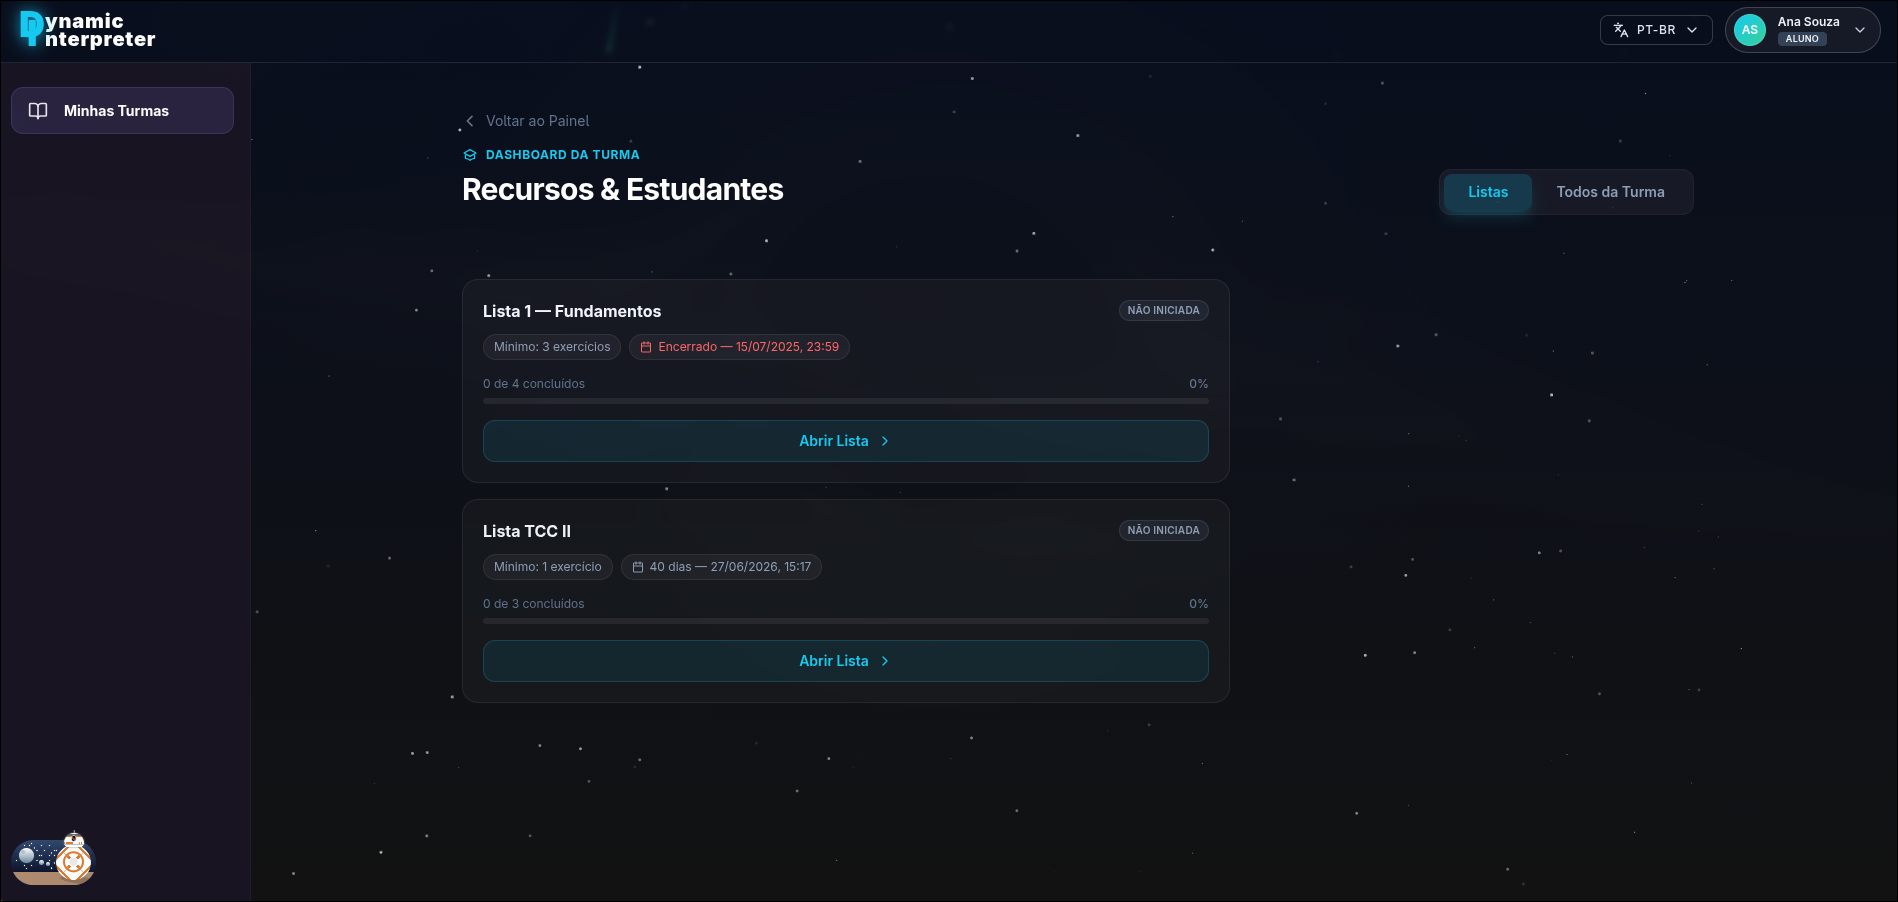
\includegraphics[width=\textwidth,height=0.34\textheight,keepaspectratio]{Aluno/Listas/Listas.png}
    \caption{Listas de exercícios de uma turma, na visão do aluno.}
    \label{fig:aluno-listas}
    \legend{Fonte: elaborado pelo autor.}
\end{figure}

Ao abrir um exercício da lista, o aluno chega à área de resolução da Figura~\ref{fig:aluno-resultado}, onde envia o programa e recebe o resultado da avaliação automatizada descrita na Seção~\ref{sec:sistema-correcao}. As submissões recebidas aparecem para o professor no detalhe da lista, em uma tabela com o aluno, o exercício, a data de envio, a situação, a nota e o botão para corrigir (Figura~\ref{fig:prof-submissoes}). A correção é feita na tela das Figuras~\ref{fig:correcao-avaliacao} e~\ref{fig:correcao-ide}.

\begin{figure}[H]
    \centering
    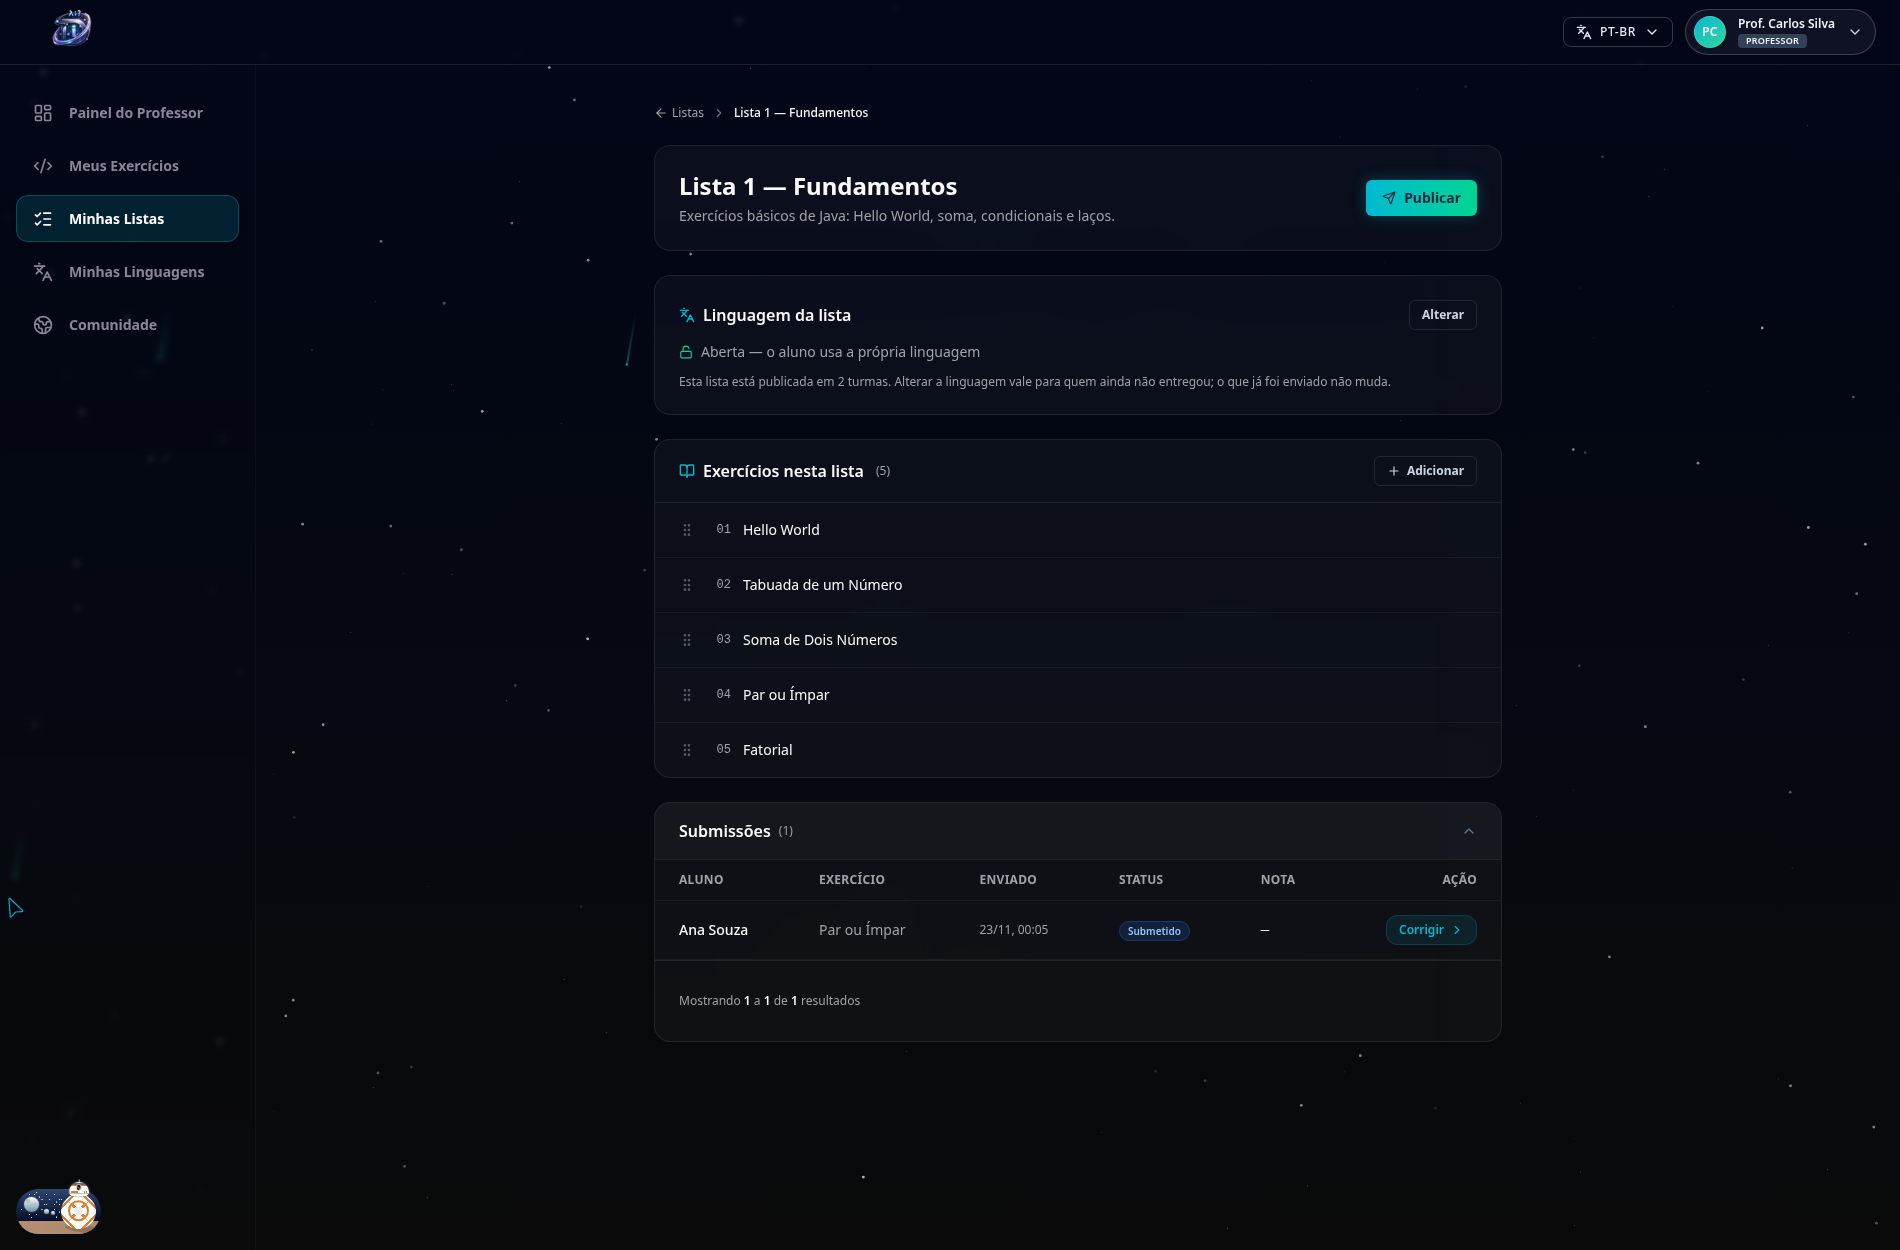
\includegraphics[width=\textwidth,height=0.34\textheight,keepaspectratio]{Professor/Listas/submissoes.png}
    \caption{Submissões recebidas no detalhe de uma lista, na visão do professor.}
    \label{fig:prof-submissoes}
    \legend{Fonte: elaborado pelo autor.}
\end{figure}

